\chapter[Prospects for $\Htautau$][Prospects for $\Htautau$]{Prospects for $\Htautau$}
\label{chap:prospects}

\begin{quote}
  Prospects for the $\Htautau$ analysis in Run-II and at the HL-LHC are described. Discussion of prospects at the HL-LHC are drawn largely from the recent ATLAS documentation on the topic~\cite{ATL-PHYS-PUB-2014-018}.
\end{quote}

\section{Run-II}
\label{sec:prospects-run2}

In Run-II, the LHC is expected to collide protons with $\sqrt{s} = 13$ TeV, a peak instantaneous luminosity of approximately $1.6\times 10^{34} \text{cm}^{-2} \text{s}^{-1}$, 25 nanosecond bunch spacing, and $\pileup\approx 40$. These data-taking conditions are much harsher than in 2012, as shown in \cref{tab:prospects-datataking}.

\begin{table}[bp] 
  \centering
  \renewcommand{\arraystretch}{1.4}
  \caption{LHC data-taking conditions in 2011 and 2012 compared with the expected data-taking conditions in 2015.}
  \begin{tabular}{c|cccc}
  \hline\hline
  Year of operations      & $\sqrt{s}$ [TeV] & peak lumi. [$\text{cm}^{-2} \text{s}^{-1}$] & bunch spacing [ns] & $\pileup$    \\
  \hline
  2011                    &  7               & $0.4\times 10^{34}$                         & 50                 & $\approx\! 10$ \\
  2012                    &  8               & $0.8\times 10^{34}$                         & 50                 & $\approx\! 20$ \\
  2015                    & 13               & $1.6\times 10^{34}$                         & 25                 & $\approx\! 40$ \\
  \hline\hline
\end{tabular}


  \label{tab:prospects-datataking}
\end{table}

The ATLAS L1 trigger rate would increase approximately five-fold if the 2012 trigger menu was ported unchanged to 2015 data-taking conditions~\cite{ATL-COM-DAQ-2014-054}. However, the L1 bandwidth is expected to increase from 75 kHz to 100 kHz, much less than this rate increase. The L1 menu must then be adapted to accommodate this.

This is especially true of triggers which rely on $\tauh$ since hadronic objects are challenging in the trigger, both in identification and calibration. An unsustainable increase of trigger rate as a function of instantaneous luminosity is shown in \cref{fig:prospects-tautriggerrates}. Multiple avenues are explored to ensure tenable trigger rates without significant loss of physics.

\begin{figure}[tp]
  \centering
  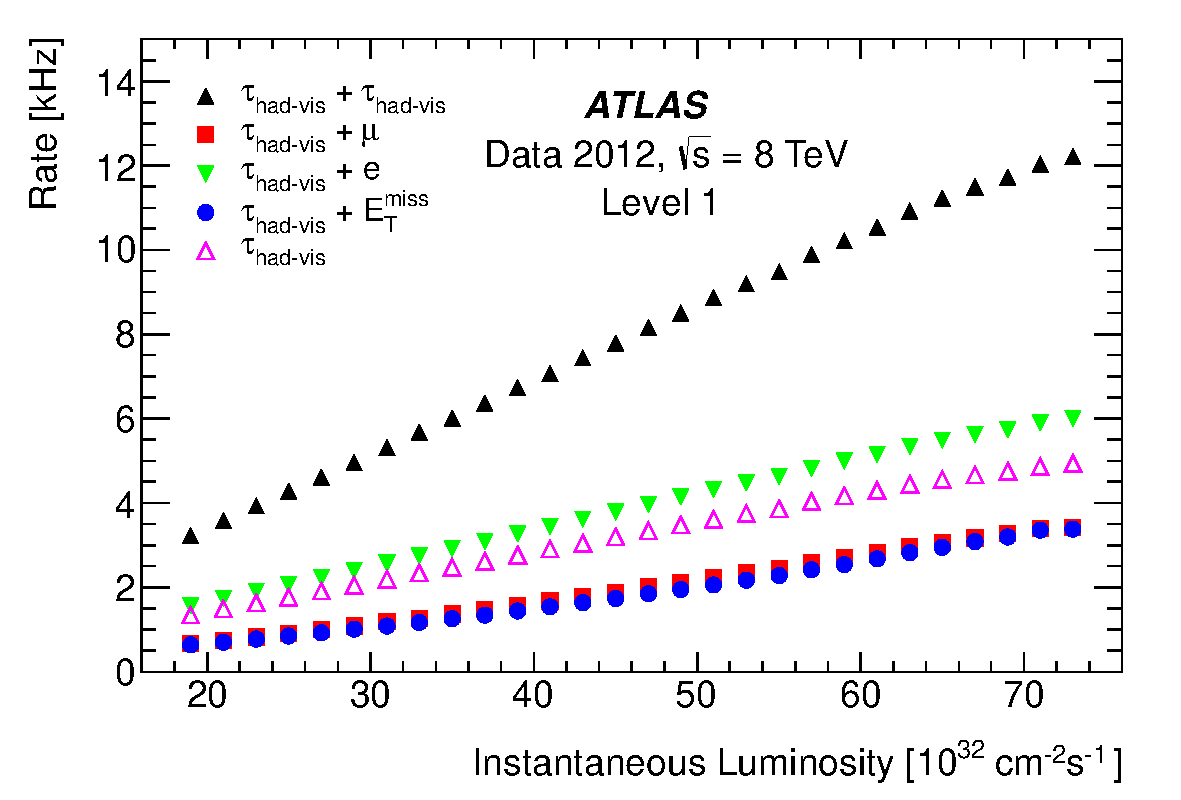
\includegraphics[width=0.48\textwidth]{figures/PERF-2013-06/fig_01a}
  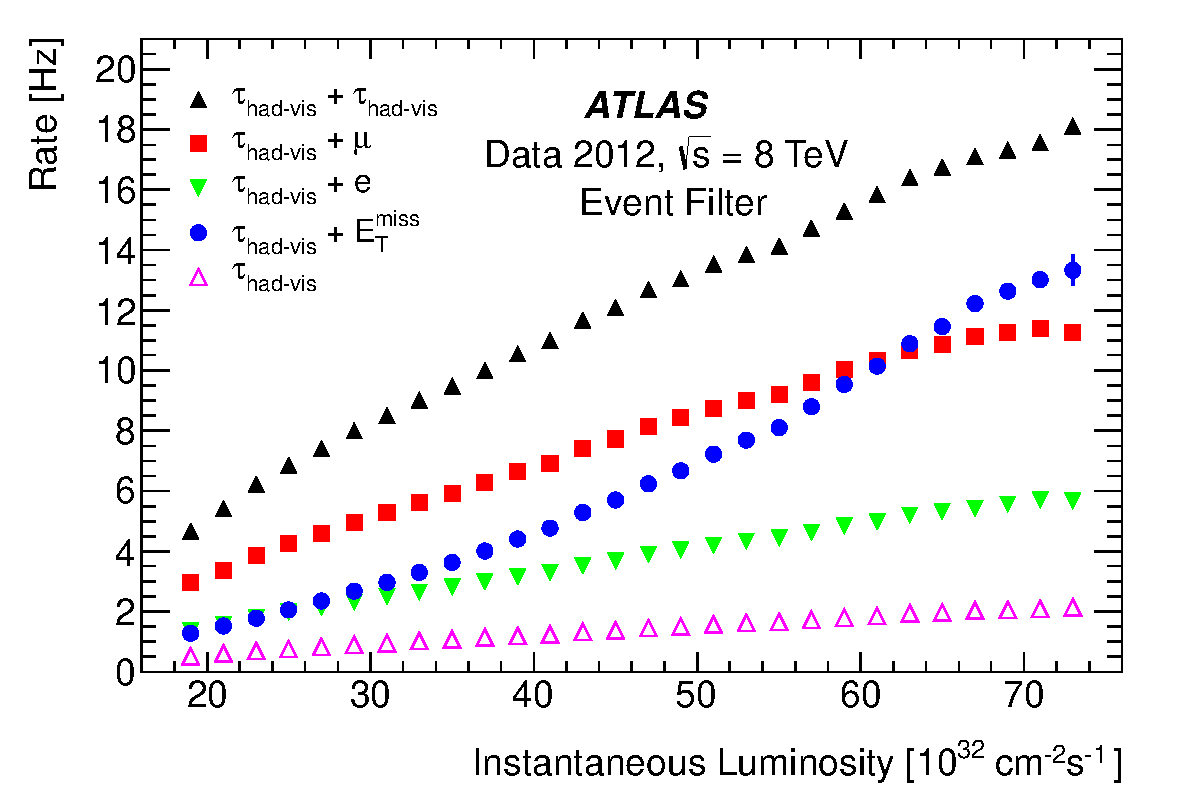
\includegraphics[width=0.48\textwidth]{figures/PERF-2013-06/fig_01b}
  \caption{Tau trigger rates in 2012 data-taking as a function of instantaneous luminosity for L1 (left) and HLT (right)~\cite{PERF-2013-06}.}
  \label{fig:prospects-tautriggerrates}
\end{figure}

\subsection{Run-I triggers for $\Htautau$}

In Run-I, only the $\Htautauhh$ analysis rely on $\tauh$ triggers for physics. The $\Htautaulh$ use single lepton triggers with an offline threshold of 26 GeV. $\LTT$ triggers are considered but ultimately dropped because they bring additional complication to the analysis without significant improvement in sensitivity. The $\Htautaull$ analysis relies on single and di-lepton triggers. The list of triggers used in 2012 data-taking, and their expected 2015 versions, is shown in \cref{tab:prospects-triggersL1} and \cref{tab:prospects-triggersHLT}.

\begin{table}[bp] 
  \centering
  \renewcommand{\arraystretch}{1.4}
  \caption{L1 triggers used in the 2012 $\Htautau$ analysis, and their expected 2015 versions, grouped by $\tautau$ decay channel.}
  \begin{tabular}{c|c|c}
  channel      & L1, 2012                    & L1, 2015 \\
  \hline\hline
  $\Htautauhh$ & \texttt{2TAU11I\_TAU15}     & no di-$\tauh$ item planned  \\
  \hline
  $\Htautaueh$ & \texttt{EM18VH}             & \texttt{EM24VHI}            \\
%               & \texttt{2TAU11I\_EM14VH}    & \texttt{TAU40\_EM15VHI}     \\
  $\Htautaumh$ & \texttt{MU20}               & \texttt{MU20}               \\
%               & \texttt{TAU8\_MU10}         & \texttt{TAU20I\_MU10}       \\
  \hline
  $\Htautauee$ & \texttt{EM18VH || 2EM10VH}  & \texttt{EM24VHI || 2EM15VH} \\
  $\Htautaumm$ & \texttt{2MU10}              & \texttt{2MU10}              \\
  $\Htautauem$ & \texttt{EM10VH\_MU6}        & \texttt{EM15VH\_MU10}       \\
\end{tabular}


  \label{tab:prospects-triggersL1}
\end{table}

\begin{table}[bp] 
  \centering
  \renewcommand{\arraystretch}{1.4}
  \caption{HLT triggers used in the 2012 $\Htautau$ analysis, and their expected 2015 versions, grouped by $\tautau$ decay channel.}
  \begin{tabular}{c|c|c}
  channel      & HLT, 2012                   & HLT, 2015 \\
  \hline\hline
  $\Htautauhh$ & \texttt{tau29Ti\_medium1\_tau20Ti\_medium1} & no di-$\tauh$ item planned \\
  \hline
  $\Htautaueh$ & \texttt{e24vhi\_medium1}                    & \texttt{e28i\_tight}                 \\
%               & \texttt{tau20Ti\_medium1\_e18vh\_medium1}   & \texttt{tau80\_medium\_e18\_medium}  \\
  $\Htautaumh$ & \texttt{mu24i\_tight}                       & \texttt{mu26i\_medium}               \\
%               & \texttt{tau20\_medium1\_mu15}               & \texttt{tau29\_medium\_mu15\_iloose} \\
  \hline
  $\Htautauee$ & \texttt{e24vhi\_medium1 || 2e12Tvh\_loose1} & \texttt{e28i\_tight || 2e17\_loose}  \\
  $\Htautaumm$ & \texttt{mu18\_tight\_mu8\_EFFS}             & \texttt{2mu14}                       \\
  $\Htautauem$ & \texttt{e12Tvh\_medium1\_mu8}               & \texttt{e17\_medium\_mu12}           \\
  \hline\hline
\end{tabular}


  \label{tab:prospects-triggersHLT}
\end{table}

\clearpage
\subsection{Run-II triggers}

Trigger options for Run-II are most critical for the $\Htautauhh$ since it relies entirely on $\tauh$ triggers. The $\Htautaull$ analysis will continue to use single and di-lepton triggers, which enjoy low thresholds and are among the most high profile triggers, and thus less likely to be cut in case of unexpectedly high rates. The $\Htautaulh$ analysis will continue to use the single lepton trigger, but the potential benefit of recovering events with leptons below the single lepton trigger thresholds could be helpful. Accordingly, only the $\Htautauhh$ and $\Htautaulh$ analyses are considered for trigger optimizations, with emphasis on $\Htautauhh$.

\subsubsection{Object thresholds}

The first and simplest option is to raise object thresholds in the trigger. Since the Run-I analysis signal regions only include event topologies with additional jets, triggering on one or two additional jets in the event is considered. To assess the impact of this, the Run-I analysis is re-run but with progressively higher thresholds on the final state objects, and the resulting sensitivity is derived. This is shown in \cref{fig:prospects-trigger-evolution}.

\begin{figure}[!htpb]
  \centering
  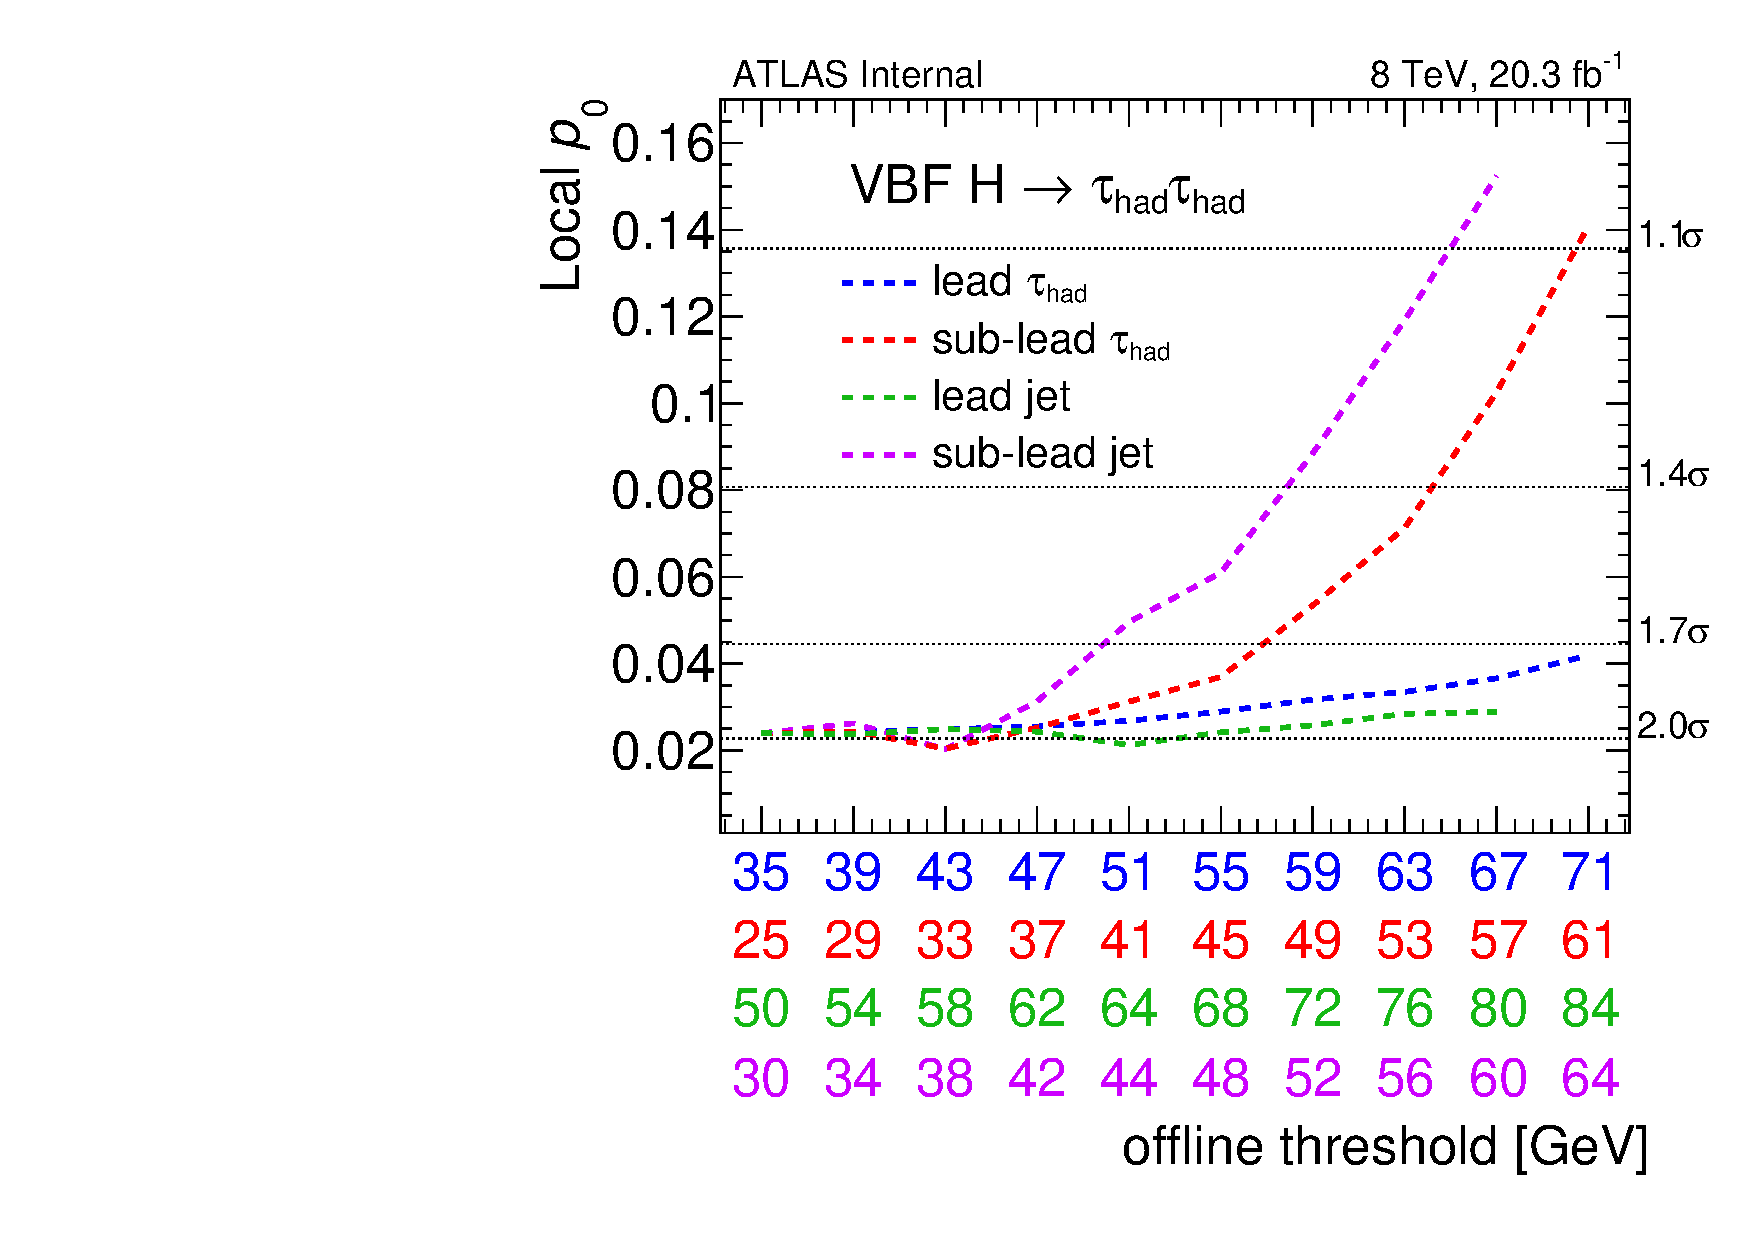
\includegraphics[width=0.48\textwidth]{figures/trigger/evolution_hadhad}
  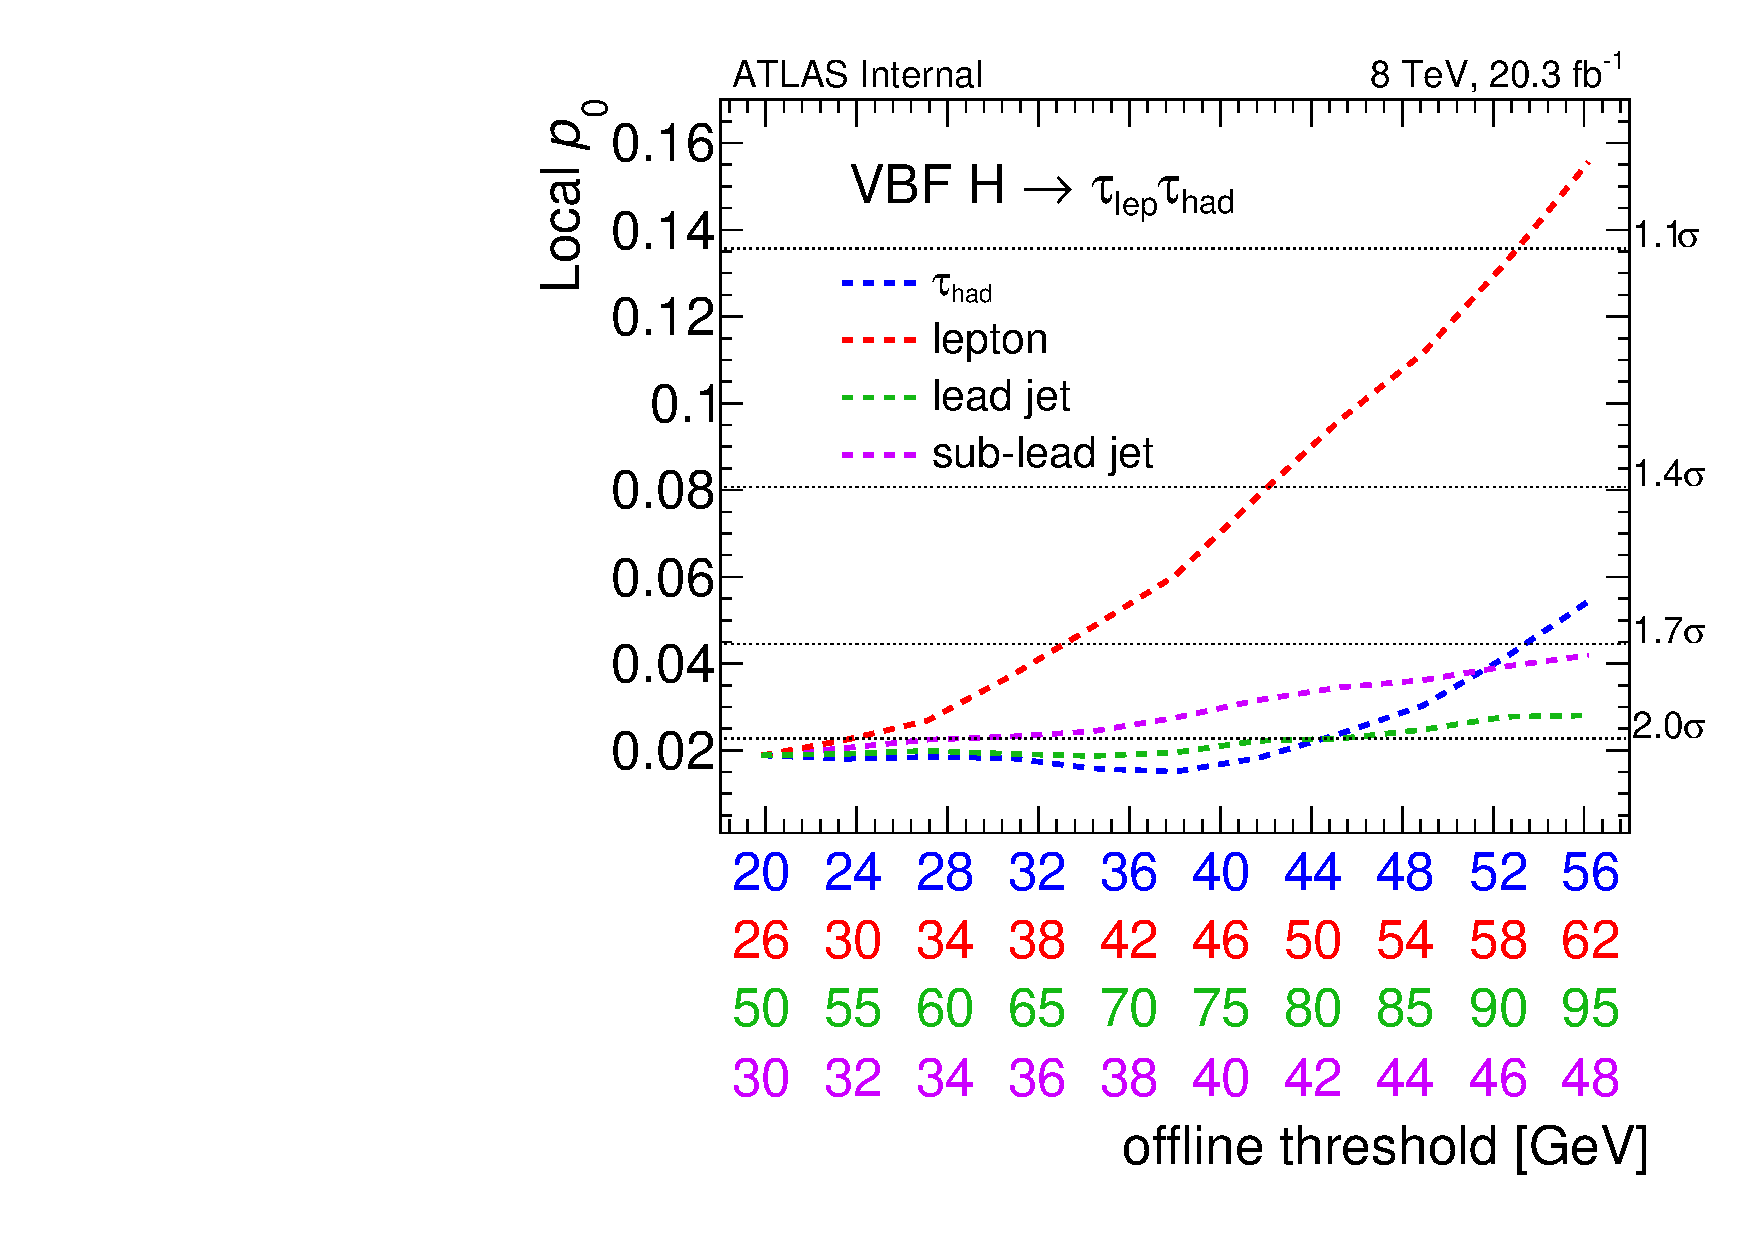
\includegraphics[width=0.48\textwidth]{figures/trigger/evolution_lephad}
  \caption{Significance ($p_0$) of the $\Htautau$ VBF category in 2012 for the $\Htautauhh$ (left) and $\Htautaulh$ (right) analyses as a function of offline or L1 threshold for various objects.}
  \label{fig:prospects-trigger-evolution}
\end{figure}

For both $\Htautauhh$ and $\Htautaulh$, triggering on the lead jet in the VBF category is promising, and triggering on the sub-lead jet is not. The lowest realistic threshold for triggering on the sub-lead jet is $15-20$ GeV at L1 ($\approx\! 50-60$ GeV offline) costs significant sensitivity in both final states. Requiring a second jet would also be inefficient for the boosted category. To trigger on the lead jet, however, an offline threshold of $\approx\! 70$ GeV ($25$ GeV at L1) does not cost significant sensitivity.

For $\Htautauhh$, raising the threshold on the lead $\tauh$ is more promising then raising the threshold on the sub-lead $\tauh$. For $\Htautaulh$, raising the threshold on the $\tauh$ is more promising than raising the threshold on the lepton.

\subsubsection{Topological requirements}

A new feature of the L1 trigger in 2015 is the ability to make topological selections, whereas in Run-I, only object multiplicity selections could be made. This topological selection are implemented via the new \texttt{L1topo} processor~\cite{ATL-DAQ-PROC-2013-039,ATL-COM-DAQ-2014-005}.

At L1, the dominant background for $\tauh$ triggers is QCD di-jet production. Topological selections can be used in various ways to suppress this process, especially in the $\Htautau$ analysis signal regions where the $\tau\tau$ system tends to be boosted.
%
\begin{description}
    \item[$\Delta\phi(\tau\tau) < X$:] \hfill \\
      QCD di-jets tend to be produced back-to-back in the transverse plane, and the $\tau\tau$ system is usually not due to transverse boost.
    \item[$\Delta\eta(\tau\tau) < X$:] \hfill \\
      QCD di-jets tend to be produced broadly in $\eta$, and the $\tautau$ system tends to have smaller $\Delta\eta$ due to longitudal boost of the $Z/H$.
    \item[$\Delta R(\tau\tau) < X$:] \hfill \\
      This combines discriminating power of $\Delta\phi(\tau\tau)$ and $\Delta\eta(\tau\tau)$.
    \item[$\pt(\tau\tau) > X$:] \hfill \\
      QCD di-jet systems tend to be produced at rest in the transverse plane, and the $\tau\tau$ system is usually not due to transverse boost.
    \item[$\mtautau > X$:] \hfill \\
      QCD di-jet systems tend to be non-resonant and low-$\pt$, and the $\tau\tau$ system is from $Z/H$ decays.
\end{description}
%
The discriminating power of these variables is shown in \cref{fig:prospects-trigger-l1topo} for $\Htautaueh$ MC versus high-pileup minimum bias MC. 

\begin{figure}[!htpb]
  \centering
  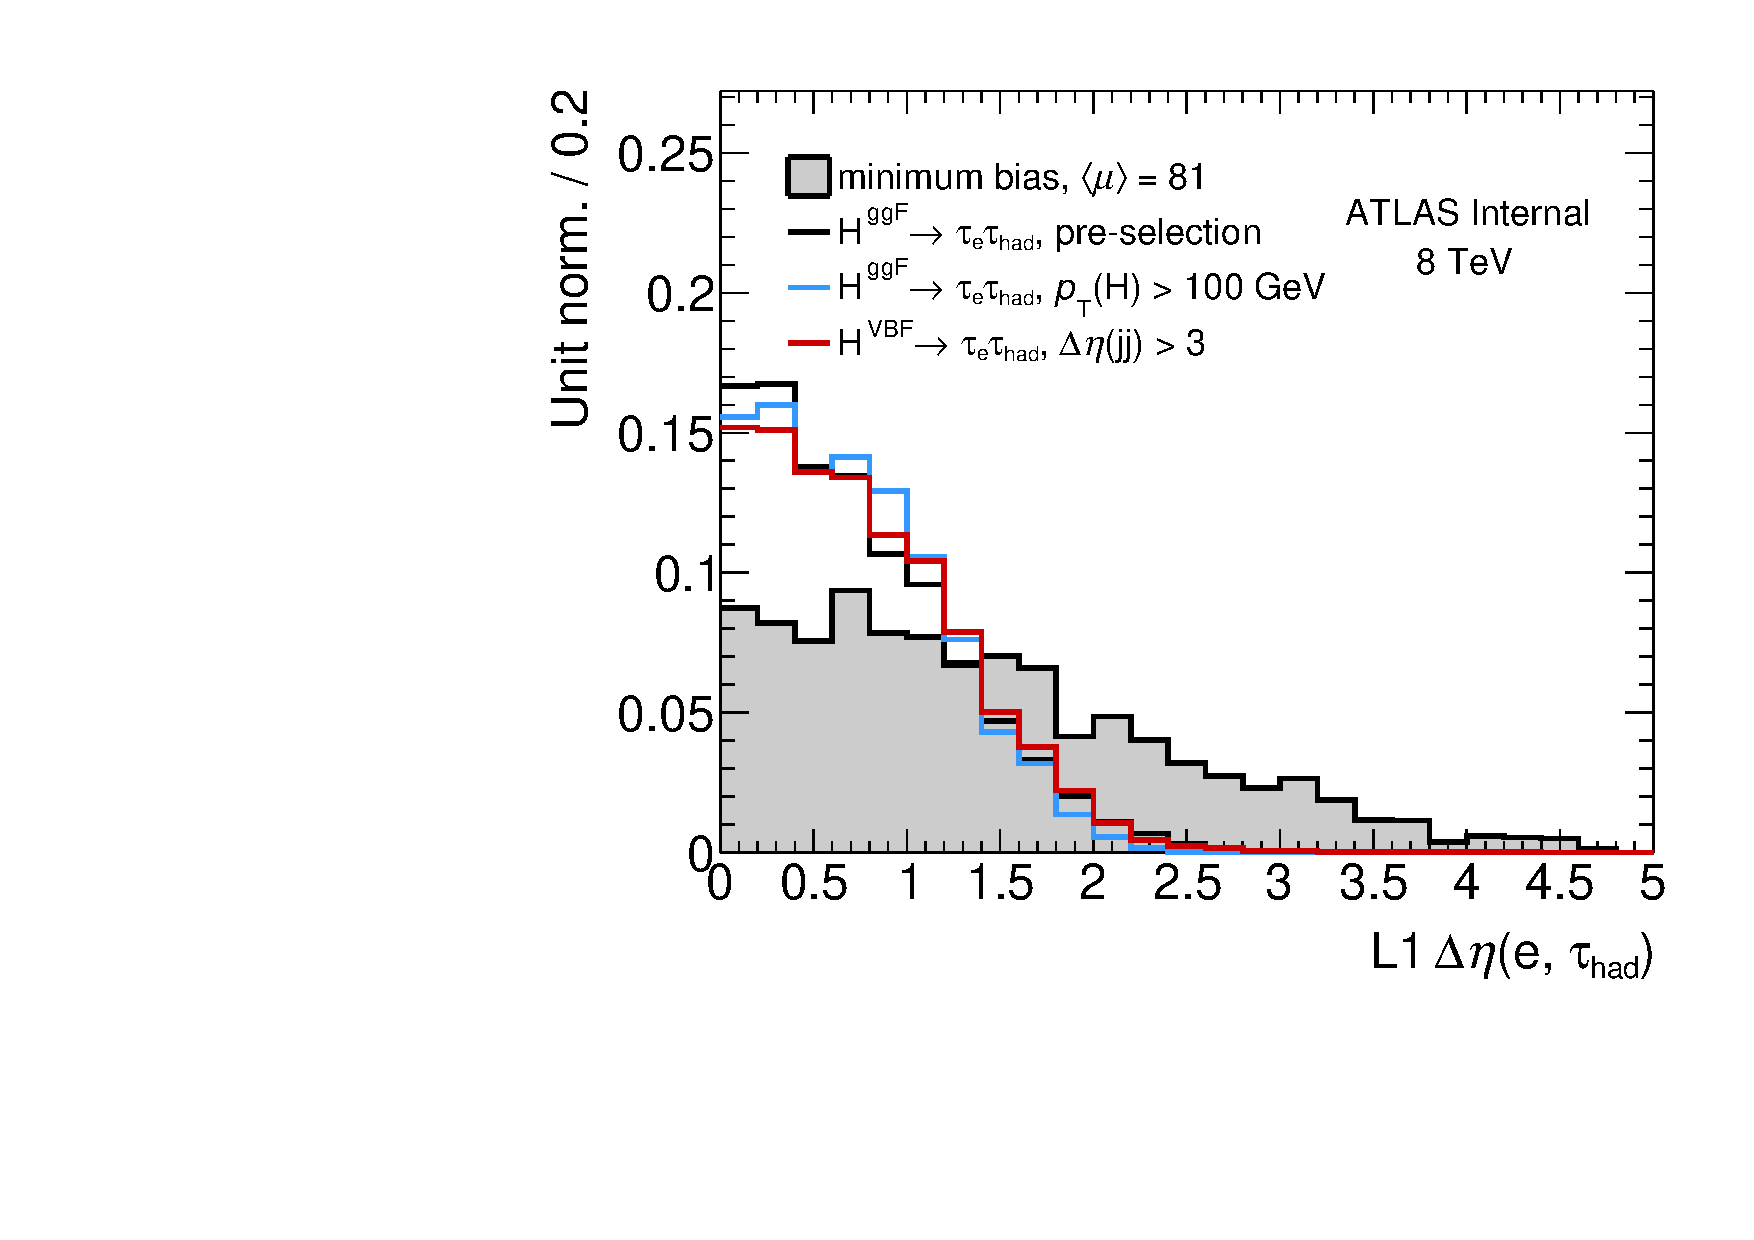
\includegraphics[width=0.32\textwidth]{figures/l1topo/taulep-deta}
  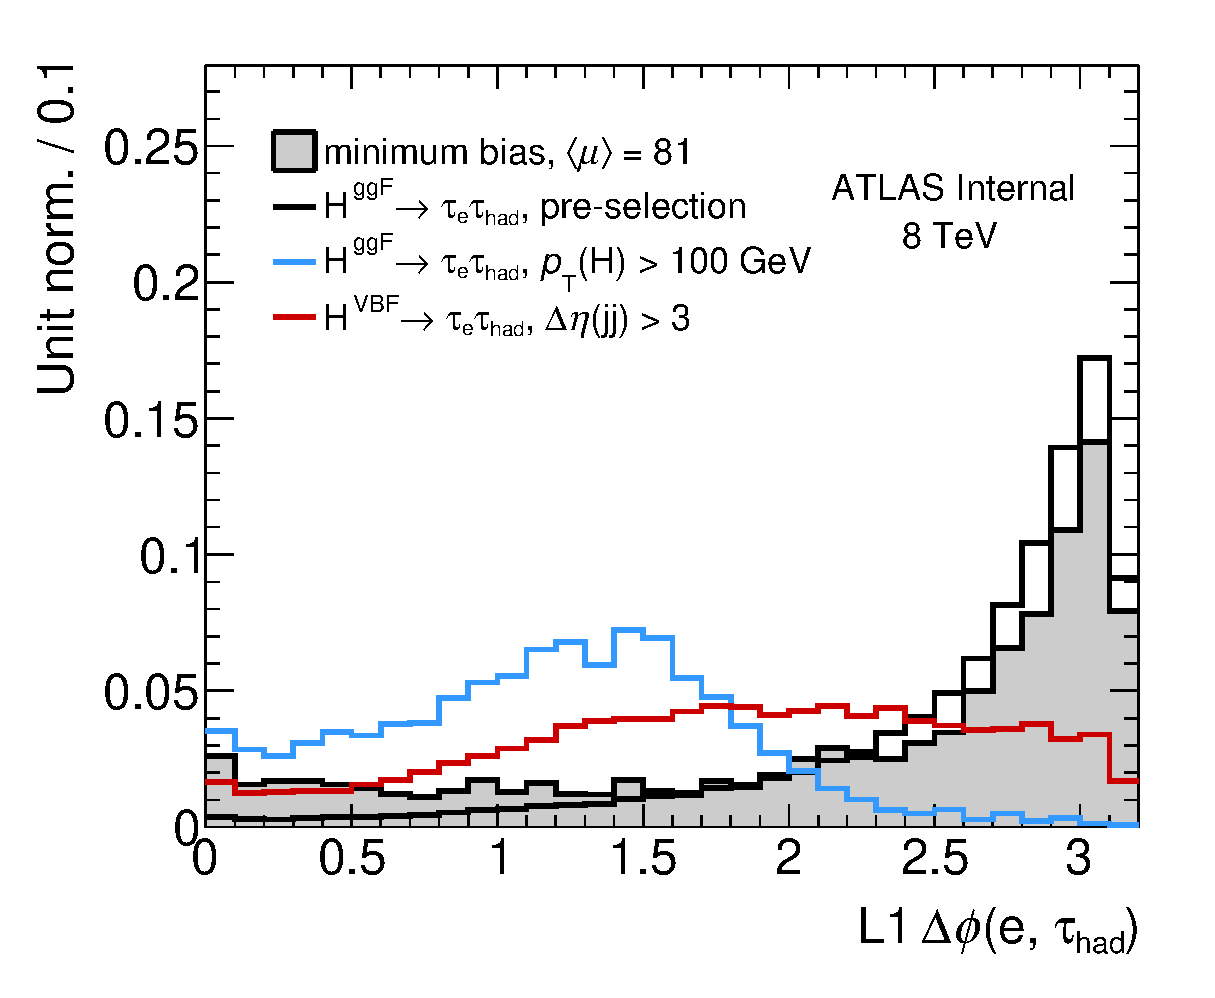
\includegraphics[width=0.32\textwidth]{figures/l1topo/taulep-dphi}
  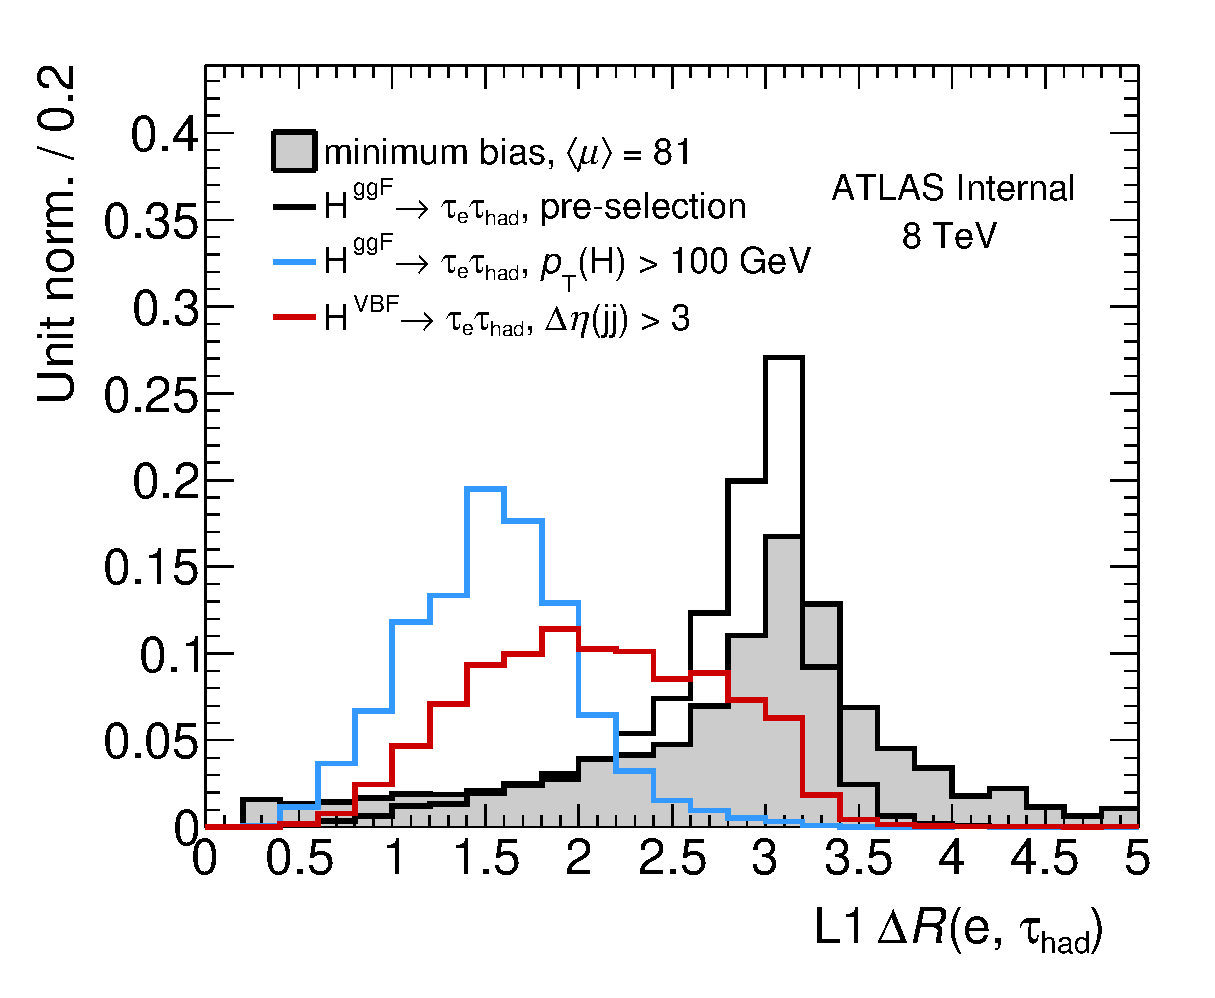
\includegraphics[width=0.32\textwidth]{figures/l1topo/taulep-dR}
  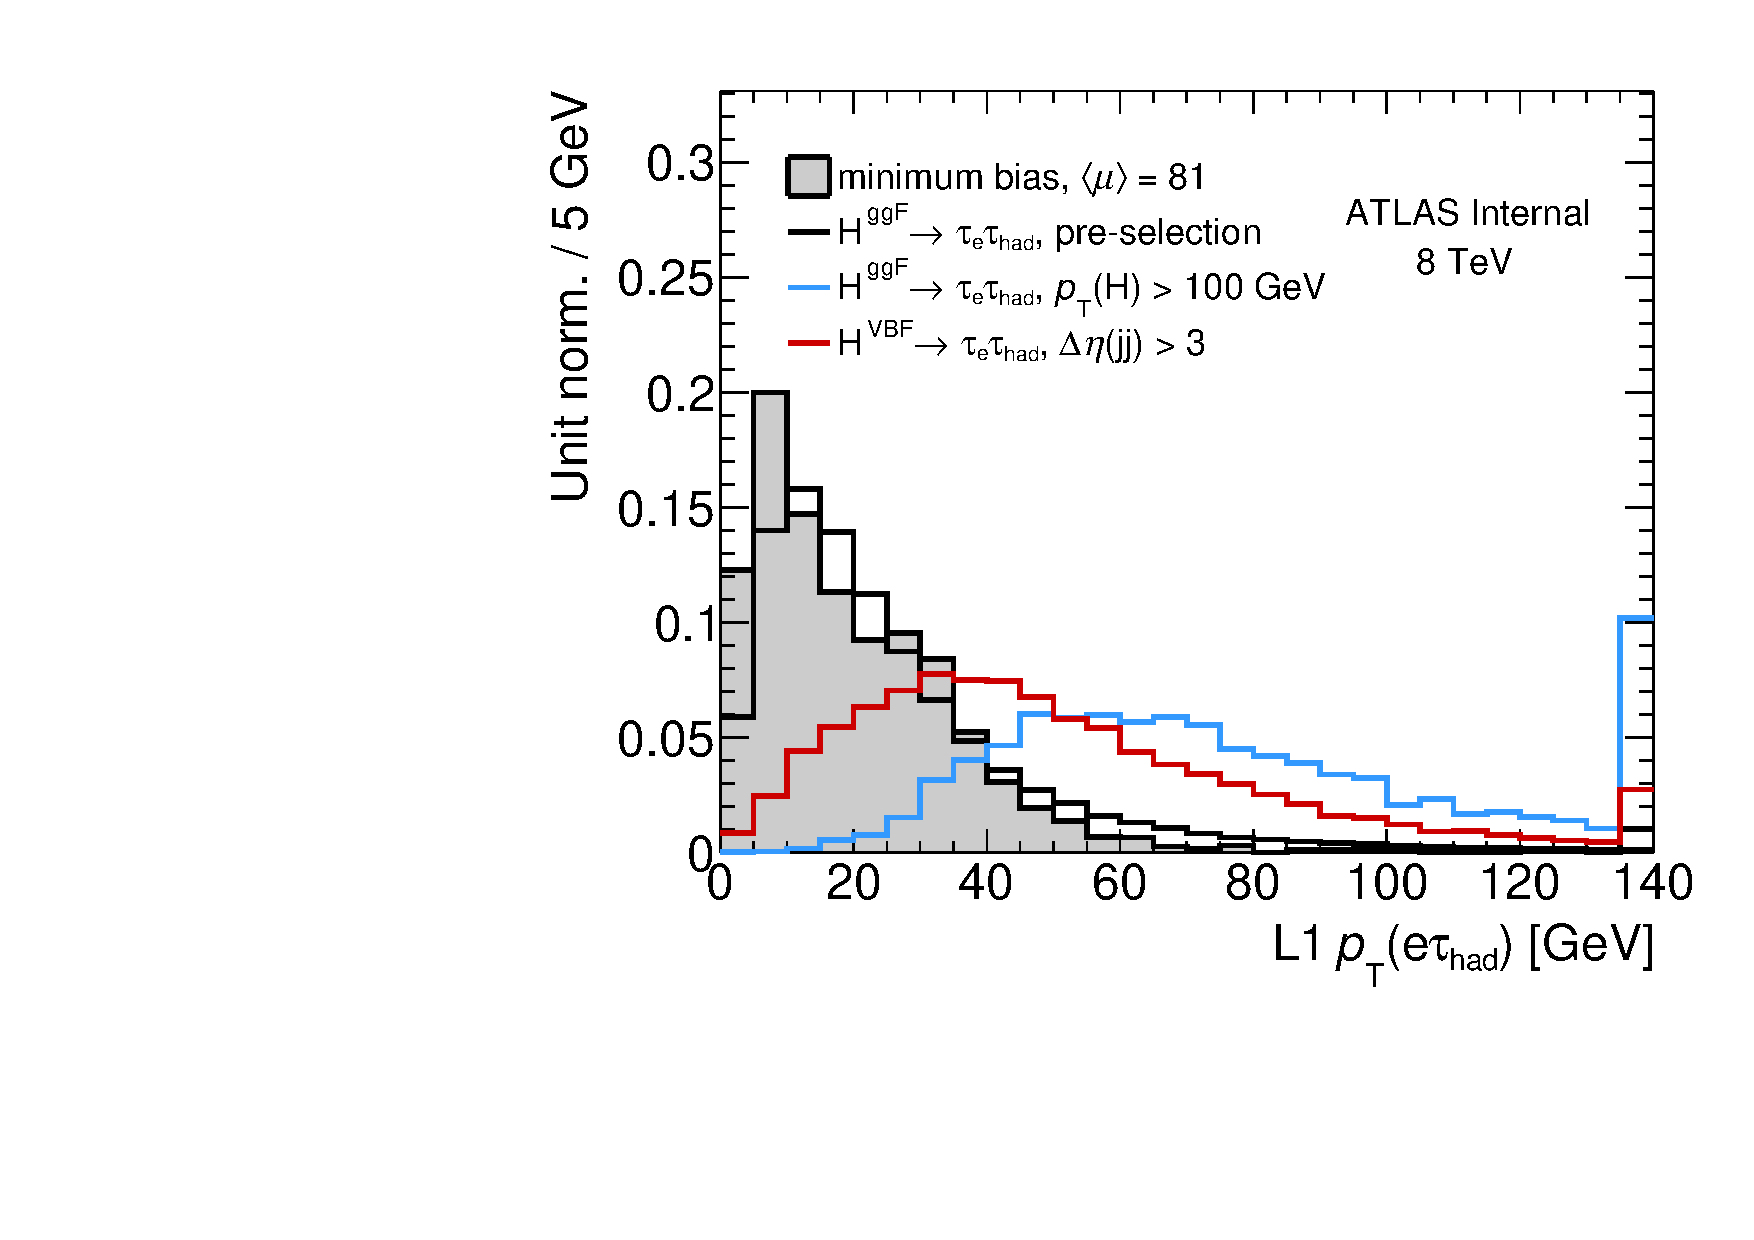
\includegraphics[width=0.32\textwidth]{figures/l1topo/ditau-pt}
  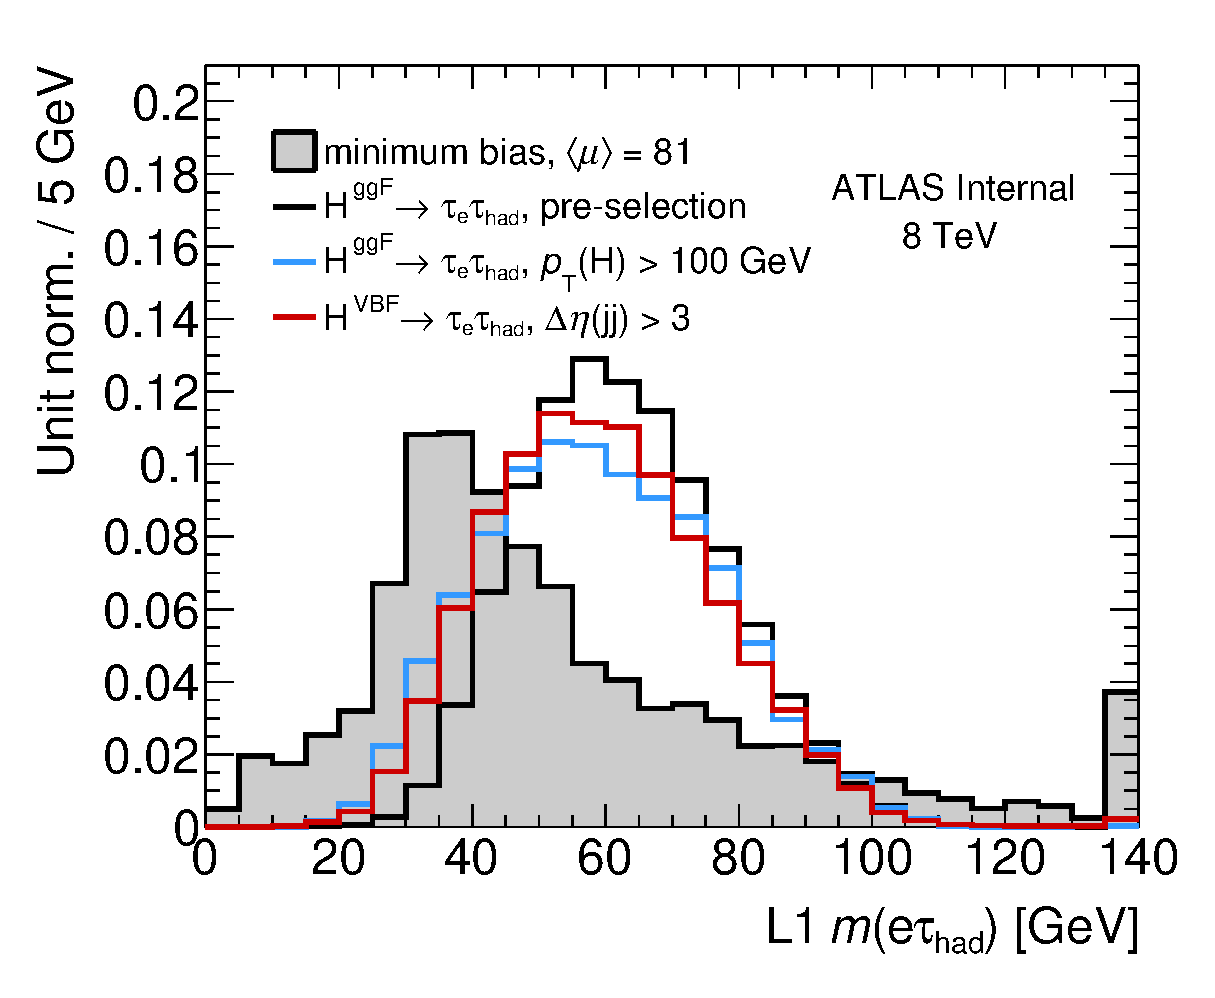
\includegraphics[width=0.32\textwidth]{figures/l1topo/ditau-m}
  \caption{Topological distributions at L1 for $\Htautaueh$ MC versus high-pileup ($\pileup=81$) minimum bias MC.}
  \label{fig:prospects-trigger-l1topo}
\end{figure}

Of these options, angular discrimination is appealing because the angular resolution for $\tauh$ at L1 is better than momentum resolution, as shown in \cref{fig:prospects-trigger-2011-angular} and \cref{fig:prospects-trigger-resolution}. Sharper efficiency turn-ons can then be expected at HLT and offline. $\Delta R(\tautau) < 2.8$ is ultimately chosen for discrimination because it combines the discriminating power of $\Delta\phi(\tautau)$ and $\Delta\eta(\tautau)$.

\begin{figure}[!htpb]
  \centering
  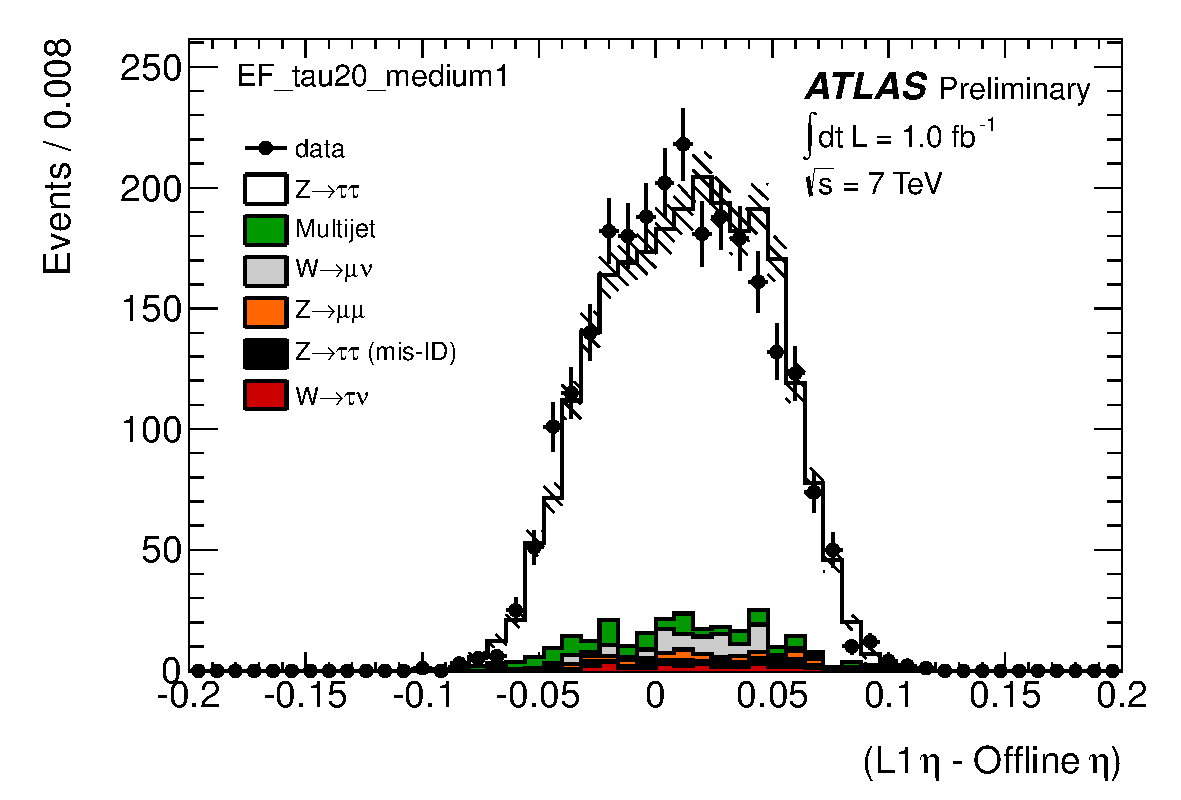
\includegraphics[width=0.48\textwidth]{figures/ATL-COM-DAQ-2012-001/c_L1_etares}
  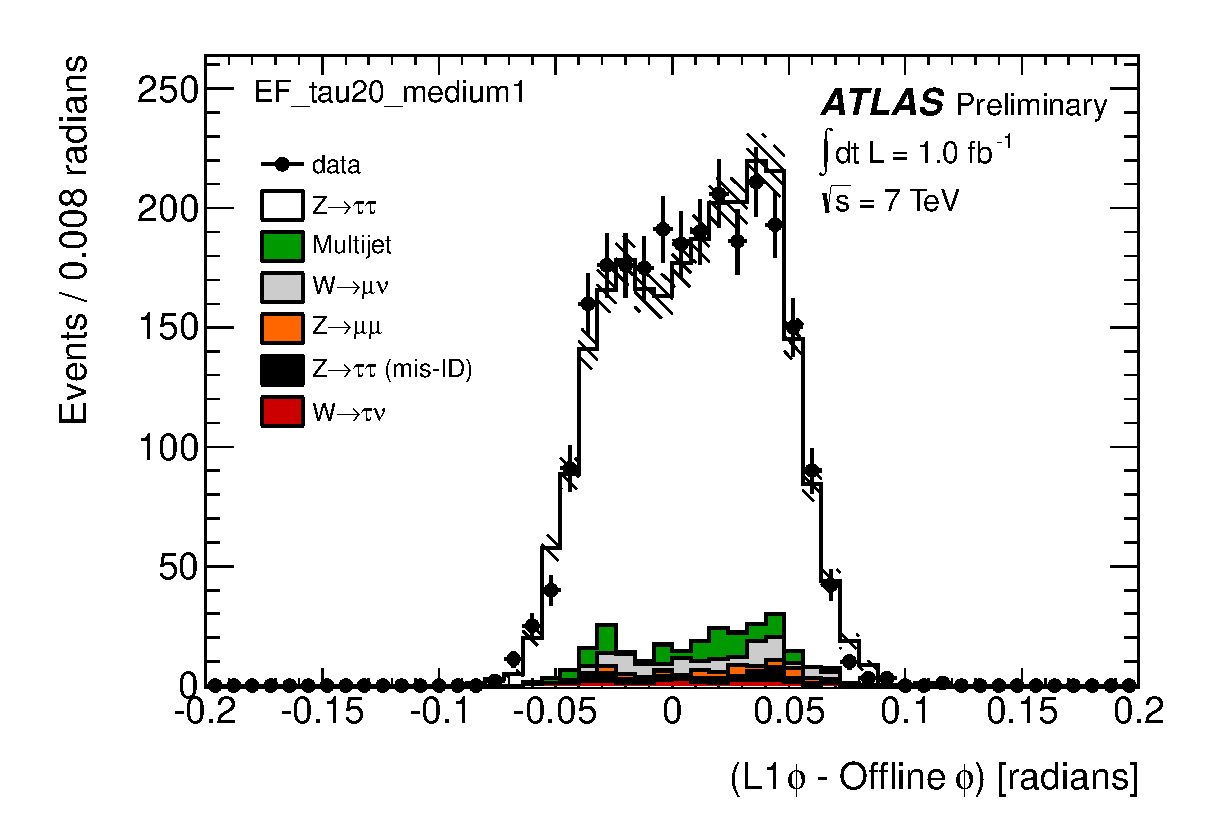
\includegraphics[width=0.48\textwidth]{figures/ATL-COM-DAQ-2012-001/c_L1_phires}
  \caption{L1 angular resolution for $\tauh$ in simulation and data~\cite{ATL-COM-DAQ-2012-001}.}
  \label{fig:prospects-trigger-2011-angular}
\end{figure}

\begin{figure}[!htpb]
  \centering
  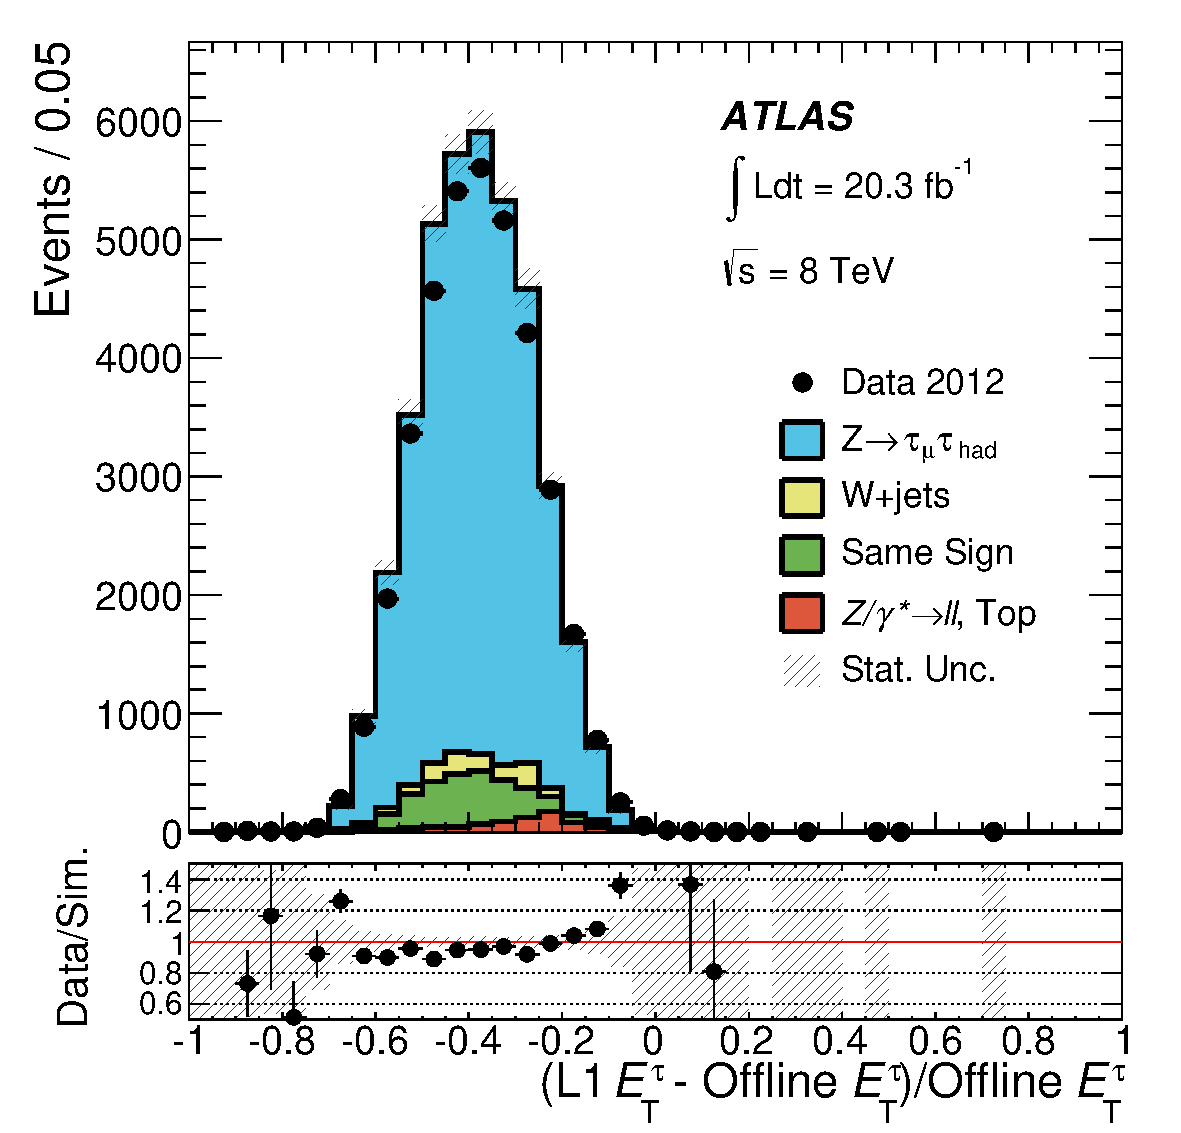
\includegraphics[width=0.48\textwidth]{figures/PERF-2013-06/fig_18a}
  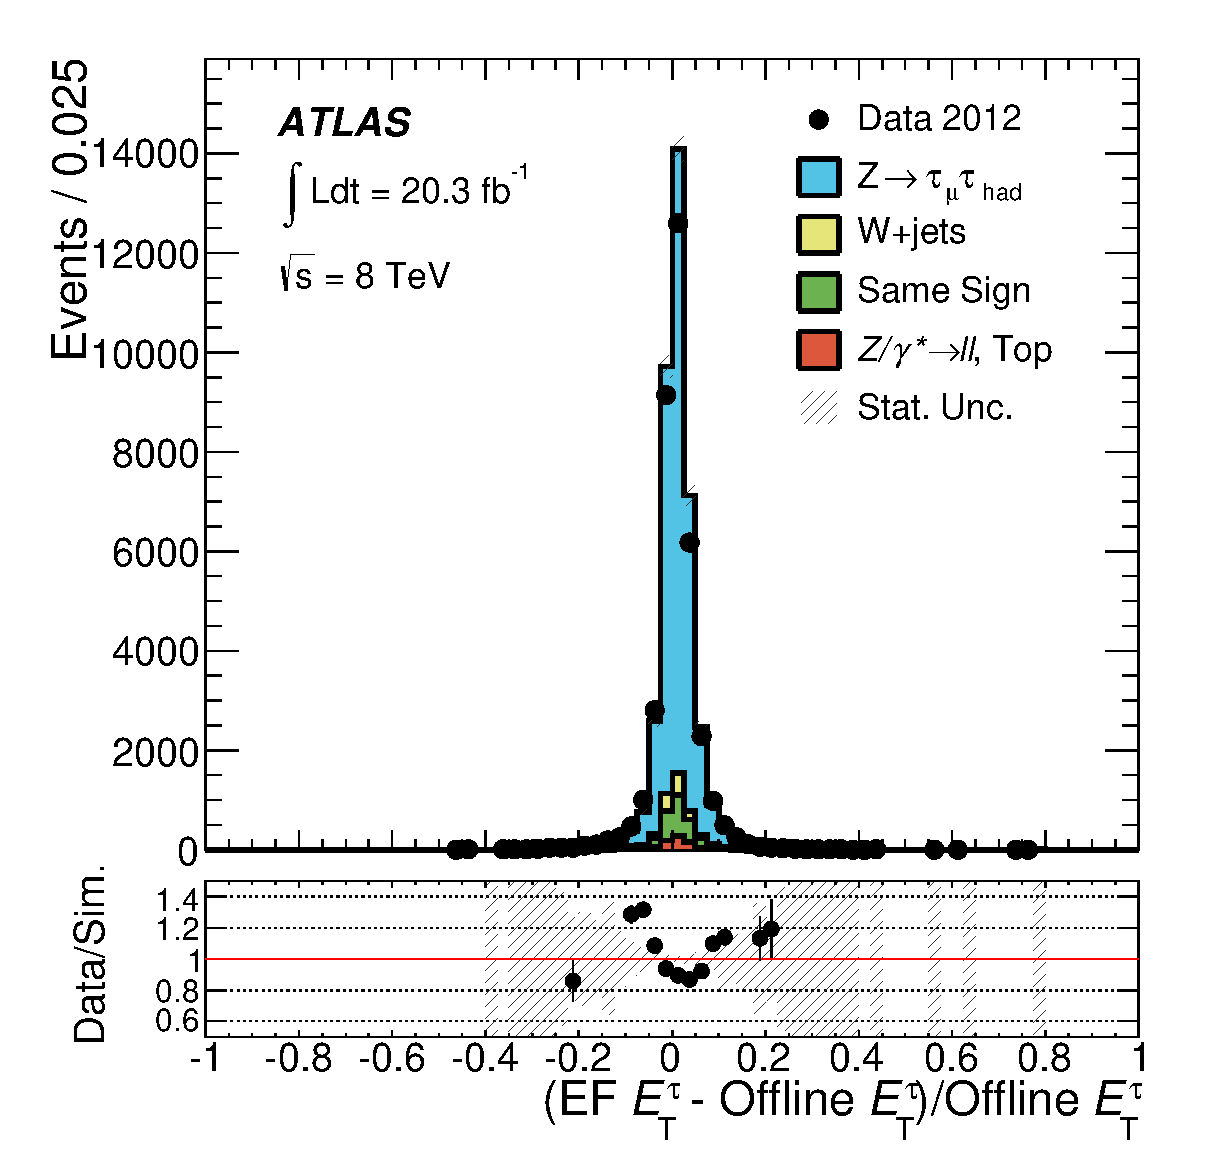
\includegraphics[width=0.48\textwidth]{figures/PERF-2013-06/fig_18c}
  \caption{Momentum resolution for $\tauh$ in simulation and data at L1 (left) and HLT (right). The resolution is significantly improved at HLT~\cite{PERF-2013-06}.}
  \label{fig:prospects-trigger-resolution}
\end{figure}

\clearpage

The impact of requiring an additional jet and $\Delta R(\tautau) < 2.8$ on the predicted 2015 L1 trigger rate is shown in \cref{tab:prospects-L1rate-evolution}. A ten-fold reduction of the rate is achieved without signicant loss of sensitivity.

\begin{table}[!htpb] 
  \centering
  \renewcommand{\arraystretch}{1.4}
  \caption{L1 trigger items and rate predictions for 2015 data-taking. A baseline L1 menu is used for calculating the unique rate.}
  \begin{tabular}{lccc}
  L1 item                 & rate [kHz] & unique rate [kHz] & notes \\
  \hline
  2TAU11                  & 181        & 147               & $\Htauhtauh$, early 2011       \\
  2TAU11I                 & 121        &  99               & $\Htauhtauh$, late 2011        \\
  TAU15I TAU11I           &  96        &  75               & $\Htauhtauh$, 2012             \\
  TAU20I TAU11I           &  69        &  48               & Raise lead $\tauh$ $\pt$     \\
  TAU20I TAU12I           &  61        &  42               & Raise sub-lead $\tauh$ $\pt$ \\
  TAU20I TAU12I J25       &  20        &  12               & Additional jet            \\
  TAU20I TAU12I J25 DR2.8 &   7.8      &   4.3             & $\dRtauhtauh < 2.8$          \\
\end{tabular}


  \label{tab:prospects-L1rate-evolution}
\end{table}

\subsubsection{Gains with $\LTT$ triggers}

To assess the potential gain in sensitivity of $\LTT$ triggers in 2015, the $\Htautaulh$ analysis is re-run in the regime below the single lepton trigger threshold with the $\LTT$ triggers running in 2012, shown in \cref{tab:prospects-LTT-2012}. Kinematic distributions are shown in \cref{fig:prospects-ltt-taus} and \cref{fig:prospects-ltt-jets}, including the final BDT discriminant.

\begin{table}[!htpb] 
  \centering
  \renewcommand{\arraystretch}{1.4}
  \caption{L1 and HLT $\LTT$ trigger items operating in 2012.}
  \begin{tabular}{c|c|c}
  channel      & L1                       & HLT \\
  \hline\hline
  $\Htautaueh$ & \texttt{2TAU11I\_EM14VH} & \texttt{tau20Ti\_medium1\_e18vh\_medium1} \\
  $\Htautaumh$ & \texttt{TAU8\_MU10}      & \texttt{tau20\_medium1\_mu15}             \\
  \hline\hline
\end{tabular}

  \label{tab:prospects-LTT-2012}
\end{table}

A simple, analytic formula for the discovery significance $Z_A$~\cite{2012.cowan.significance} gives $0.7\sigma$ for the $\LTT$ triggered category. This is not a significant improvment over the single lepton triggered regime.

\clearpage
\begin{figure}[tp]
  \centering
  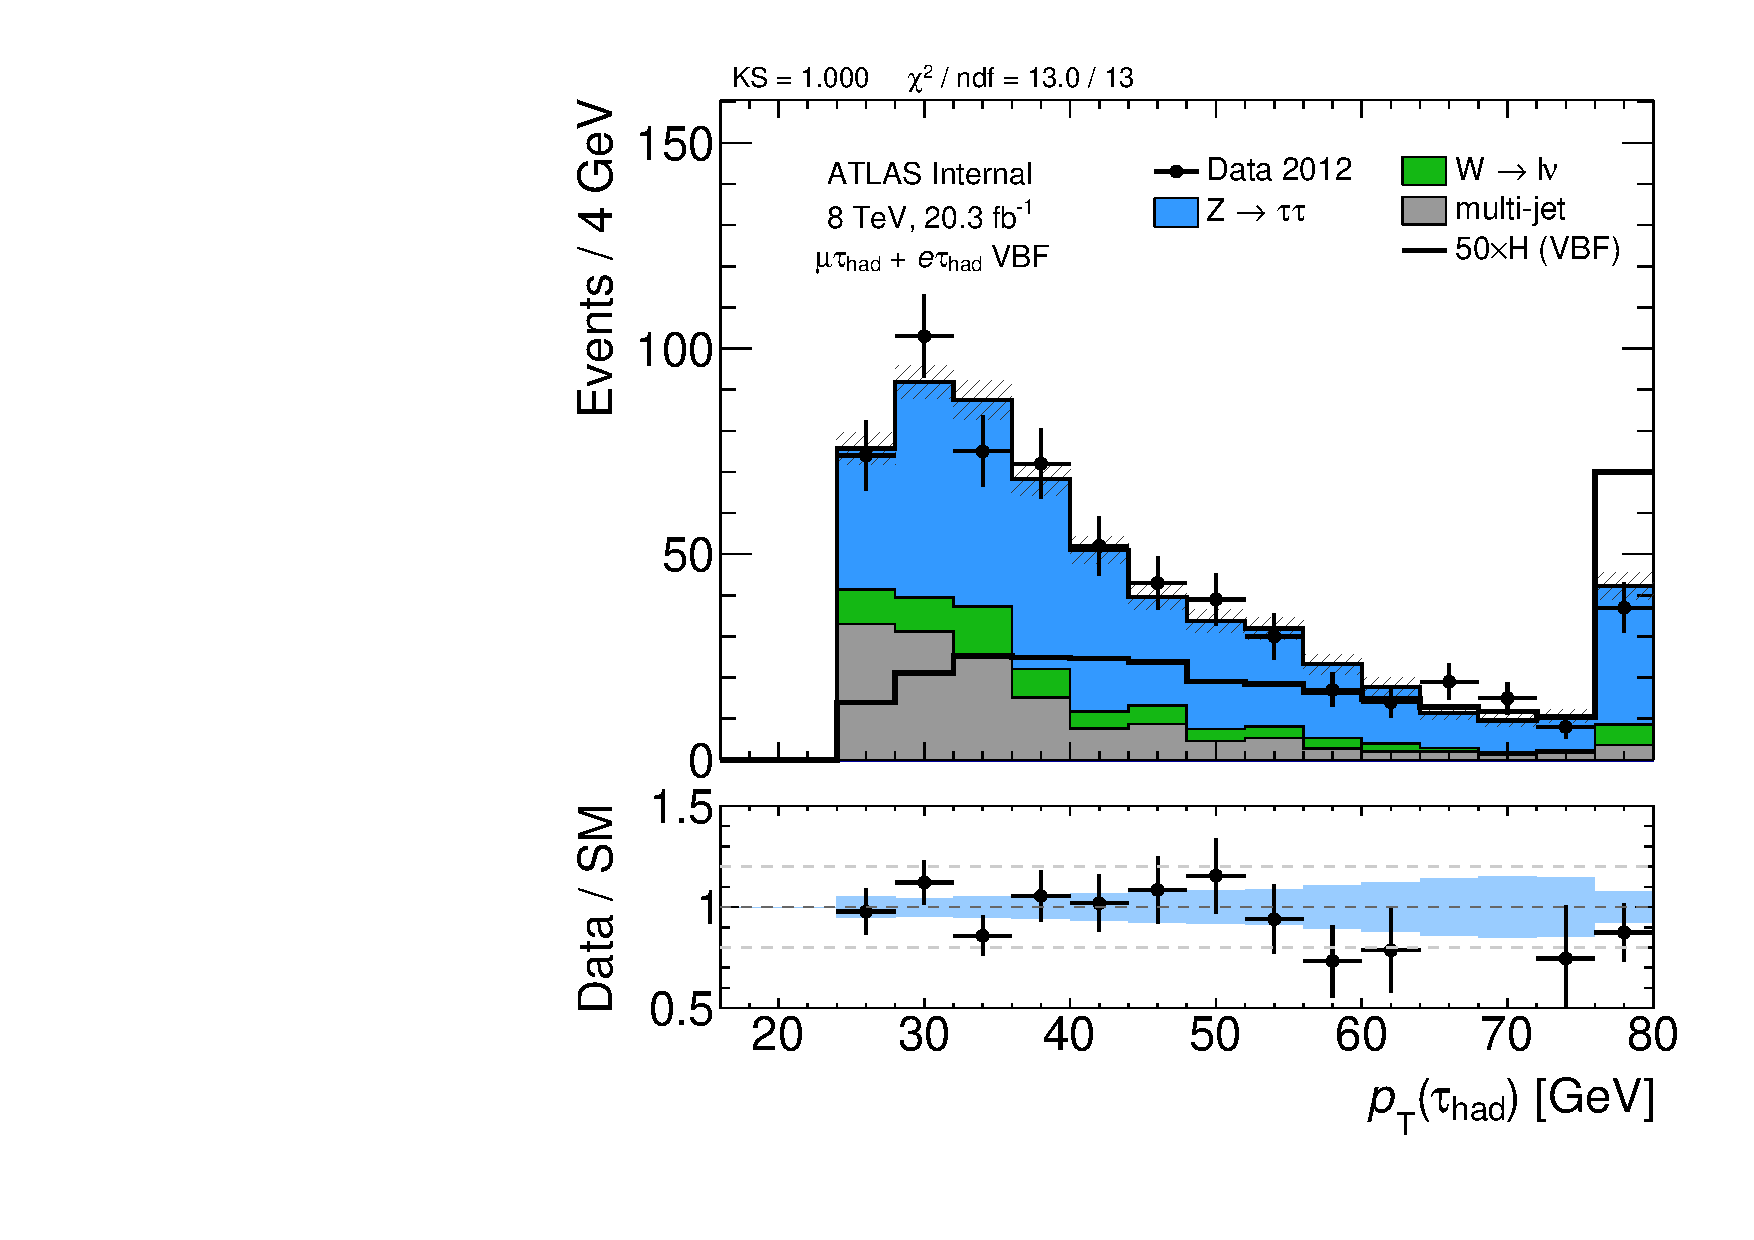
\includegraphics[width=0.32\textwidth]{figures/vbf-LTT/tau-pt}
  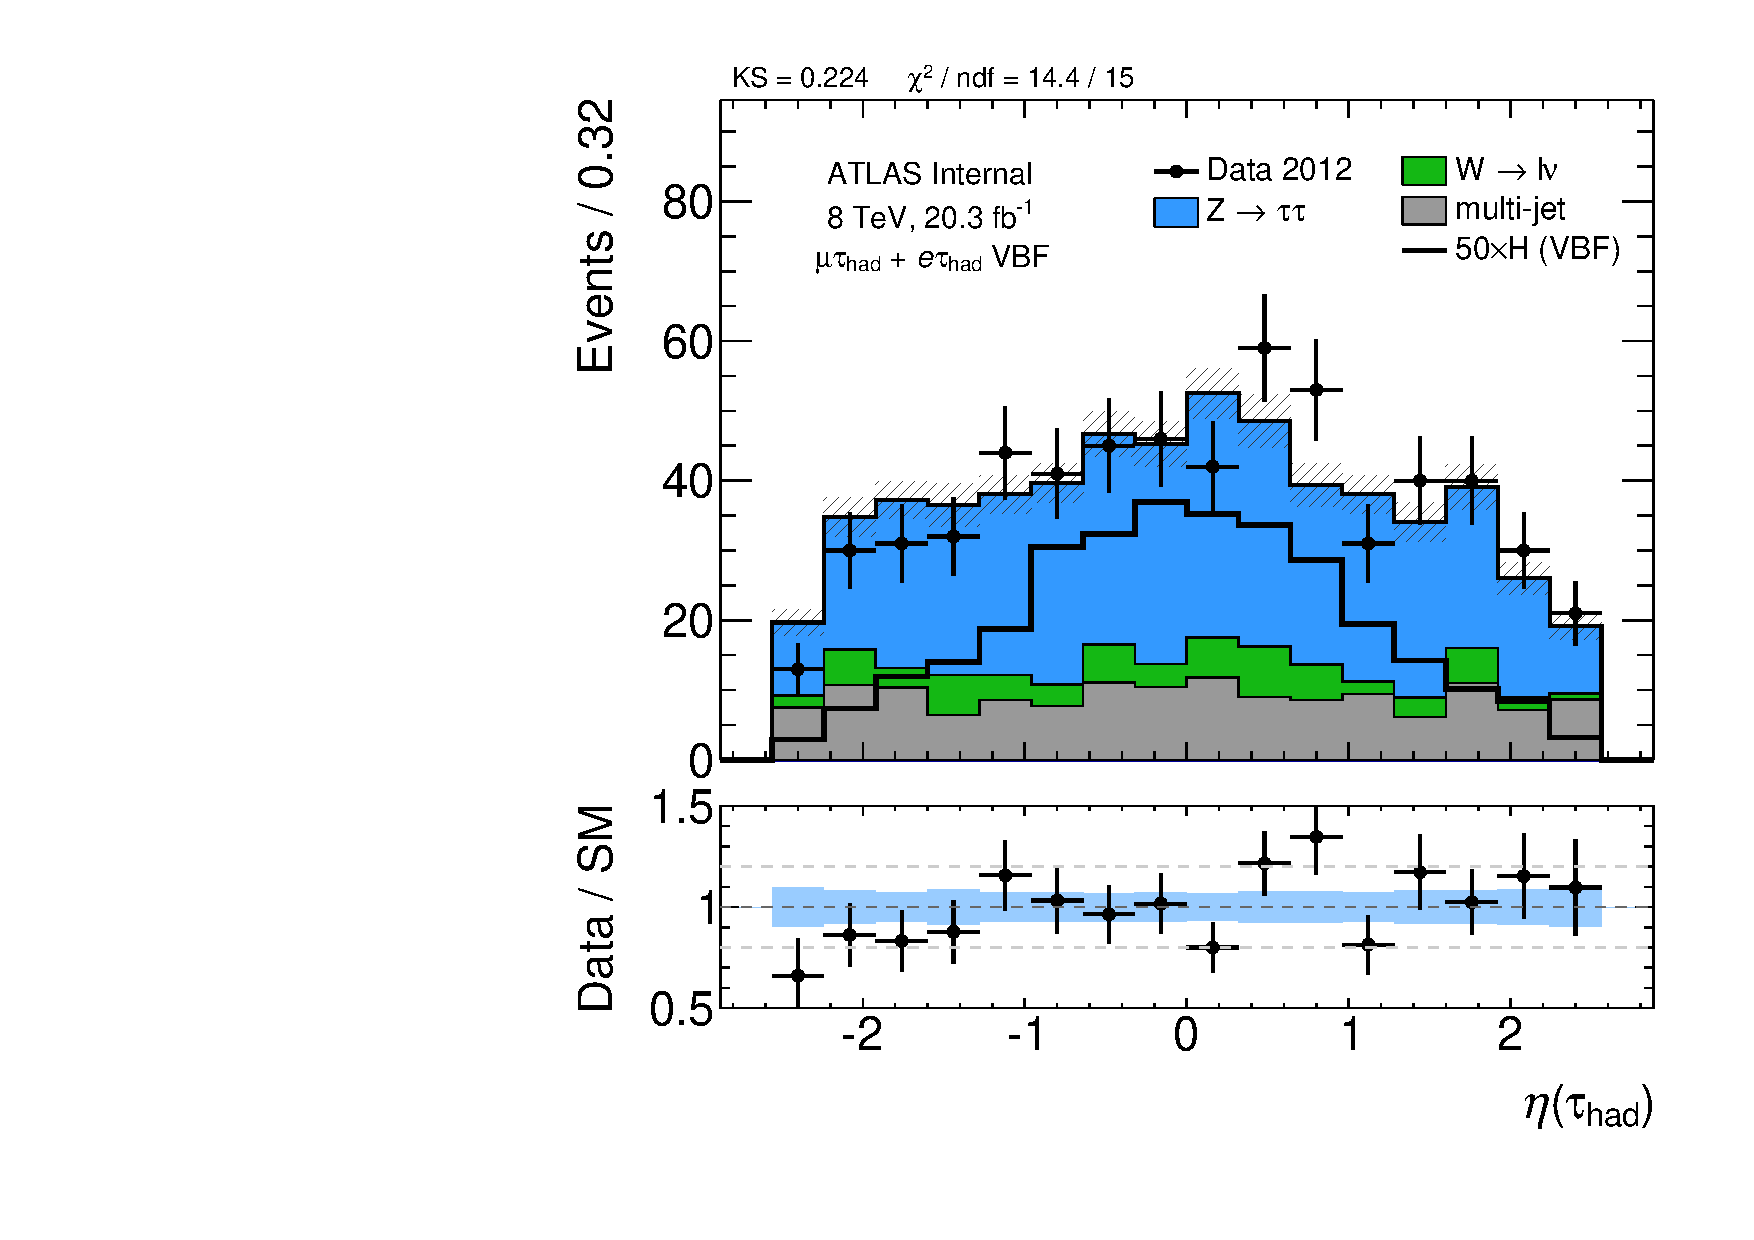
\includegraphics[width=0.32\textwidth]{figures/vbf-LTT/tau-eta}
  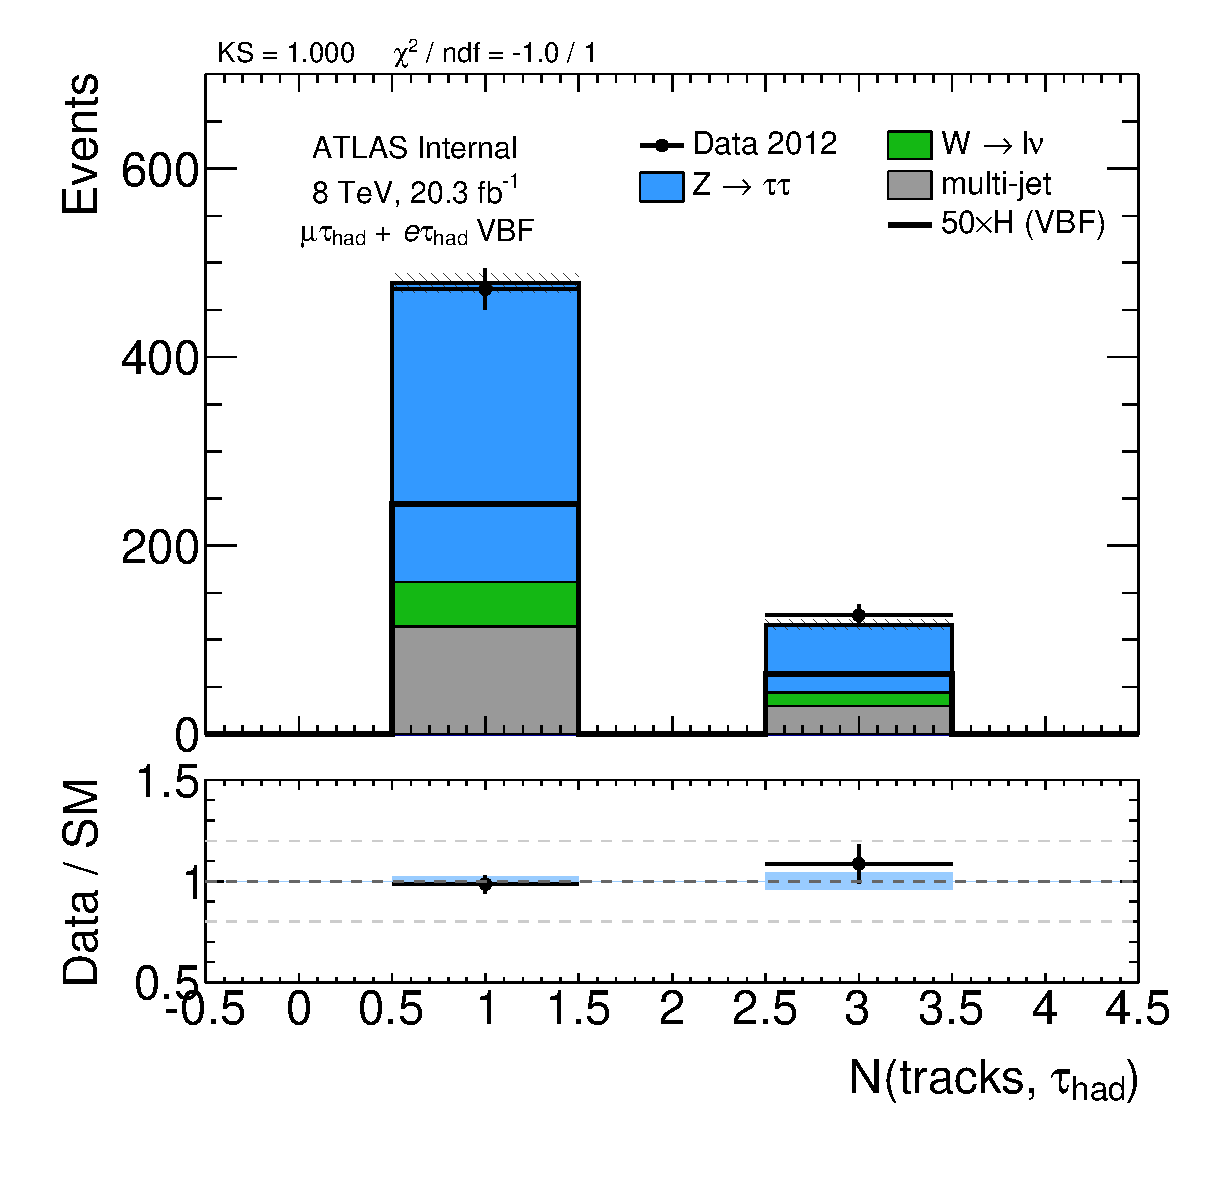
\includegraphics[width=0.32\textwidth]{figures/vbf-LTT/tau-numTrack}
  % --------------
  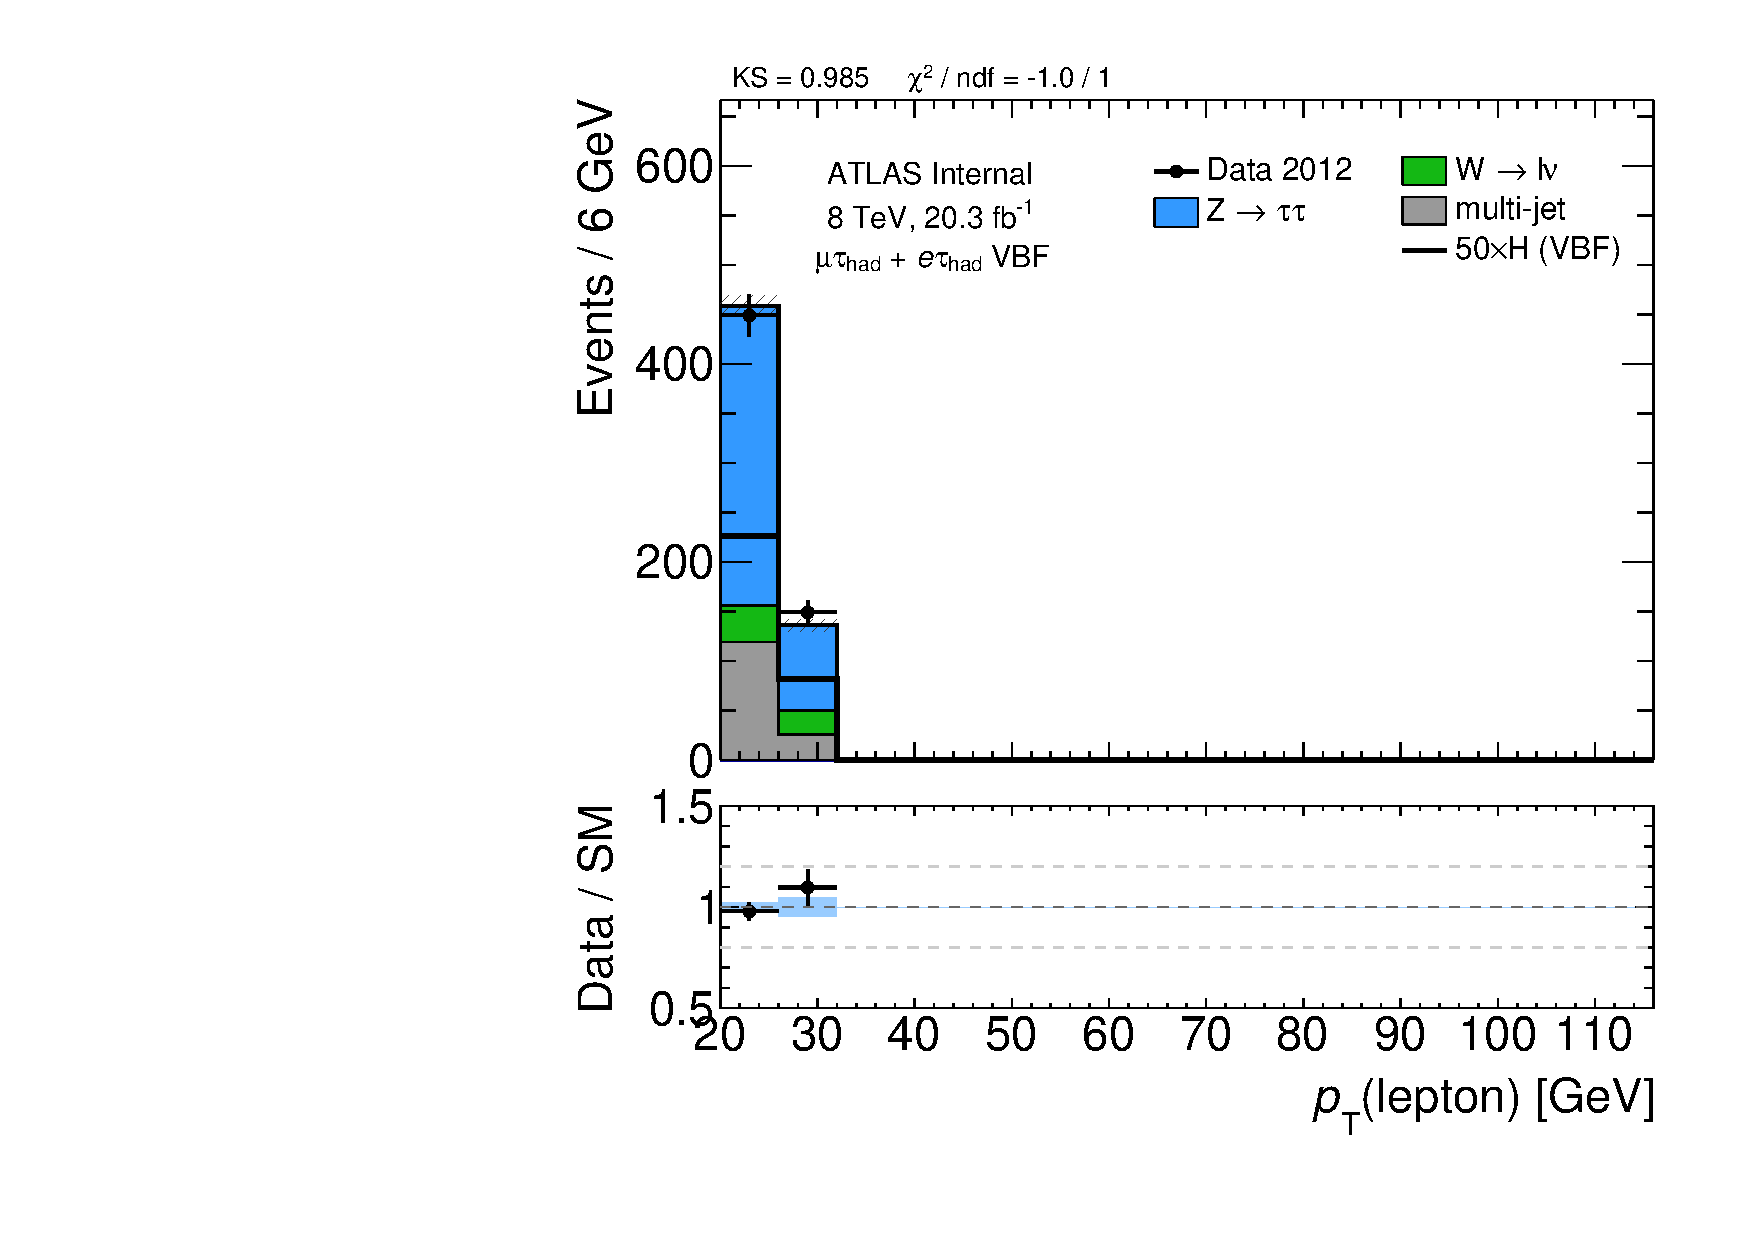
\includegraphics[width=0.32\textwidth]{figures/vbf-LTT/lep-pt-hi}
  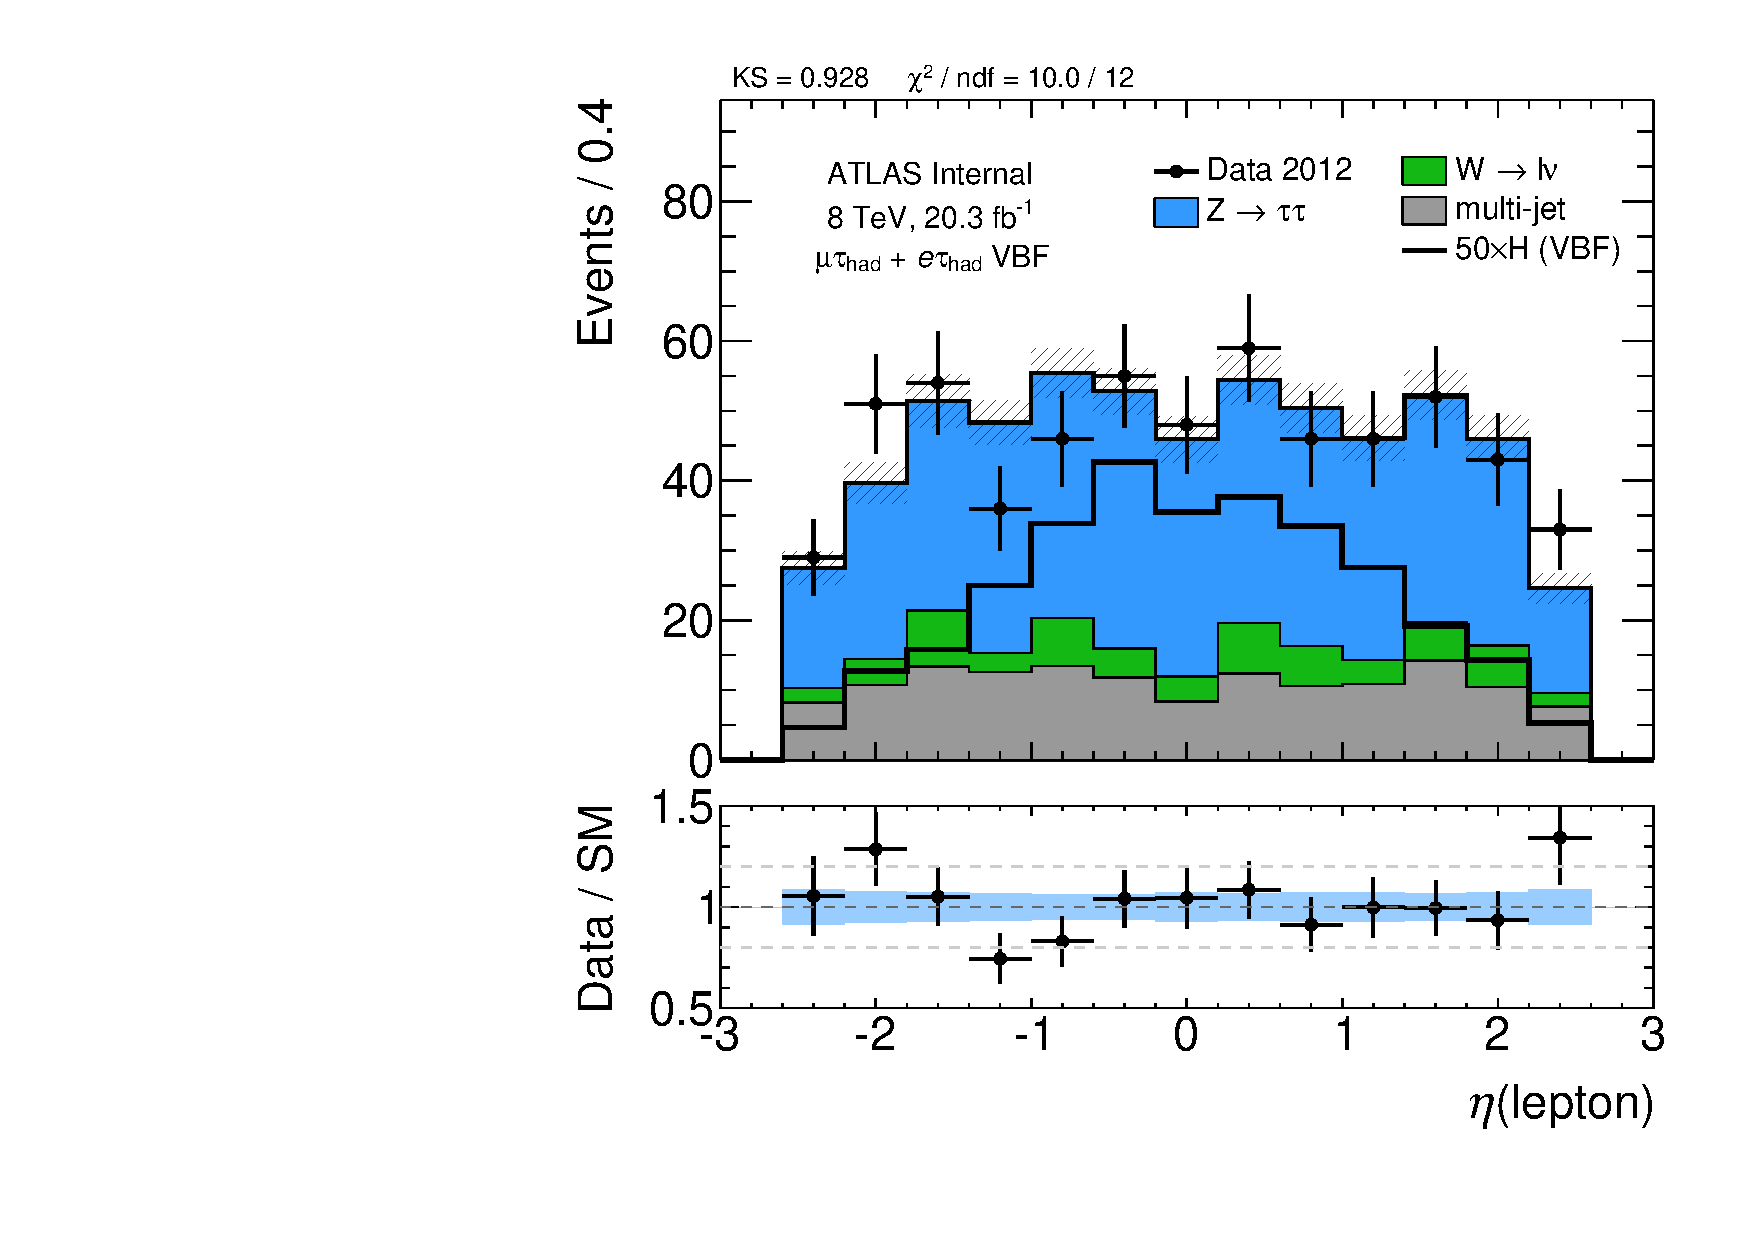
\includegraphics[width=0.32\textwidth]{figures/vbf-LTT/lep-eta}
  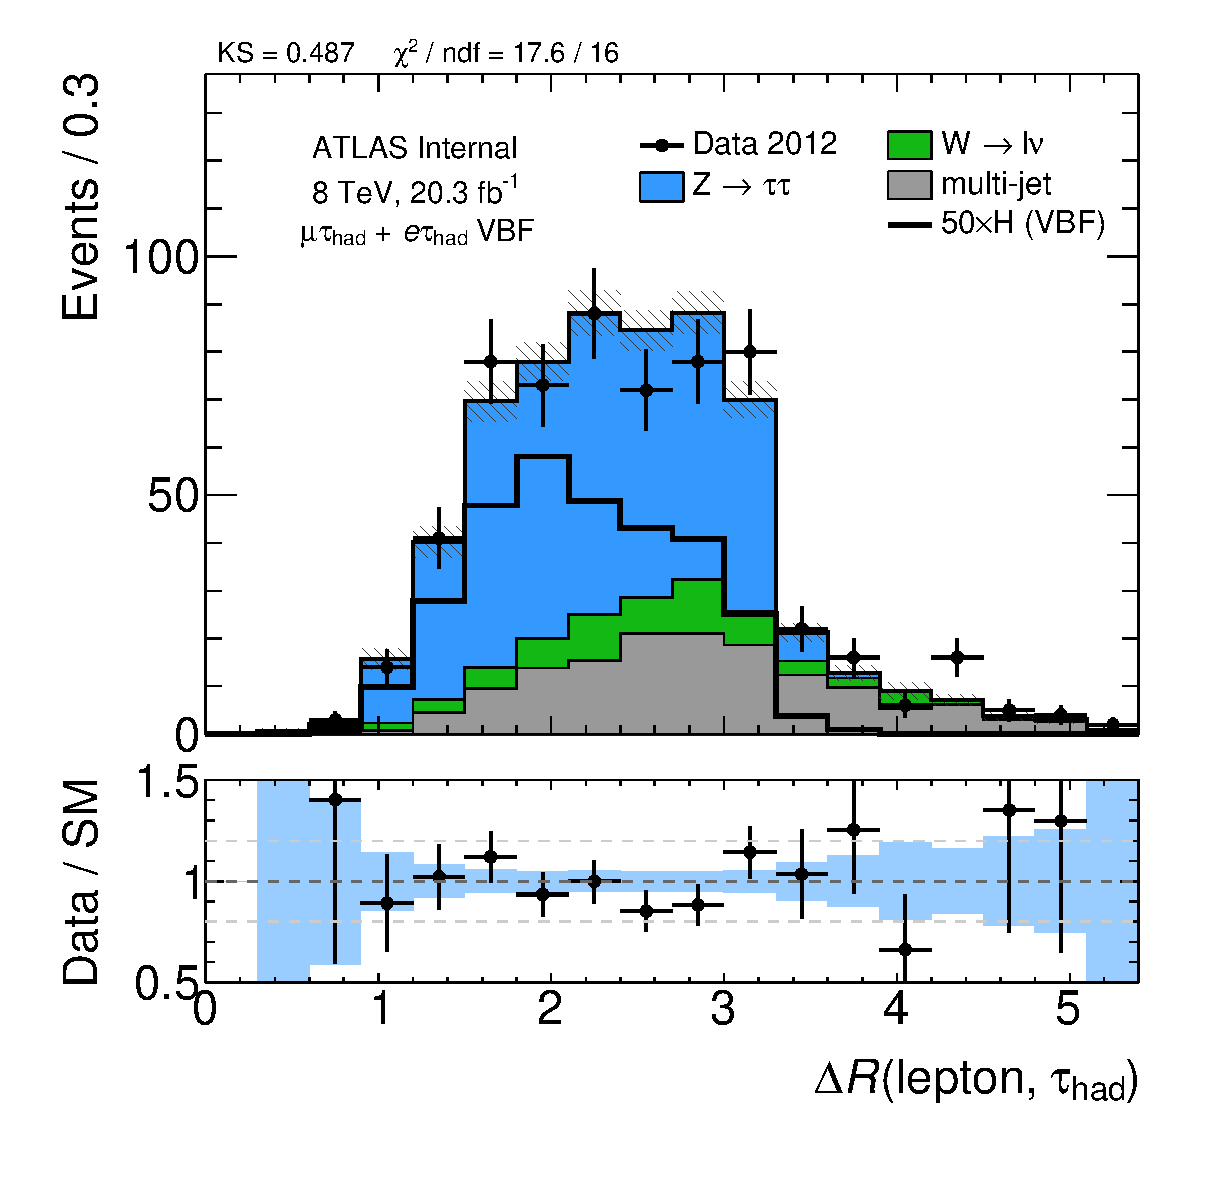
\includegraphics[width=0.32\textwidth]{figures/vbf-LTT/taulep-dR}
  % --------------
  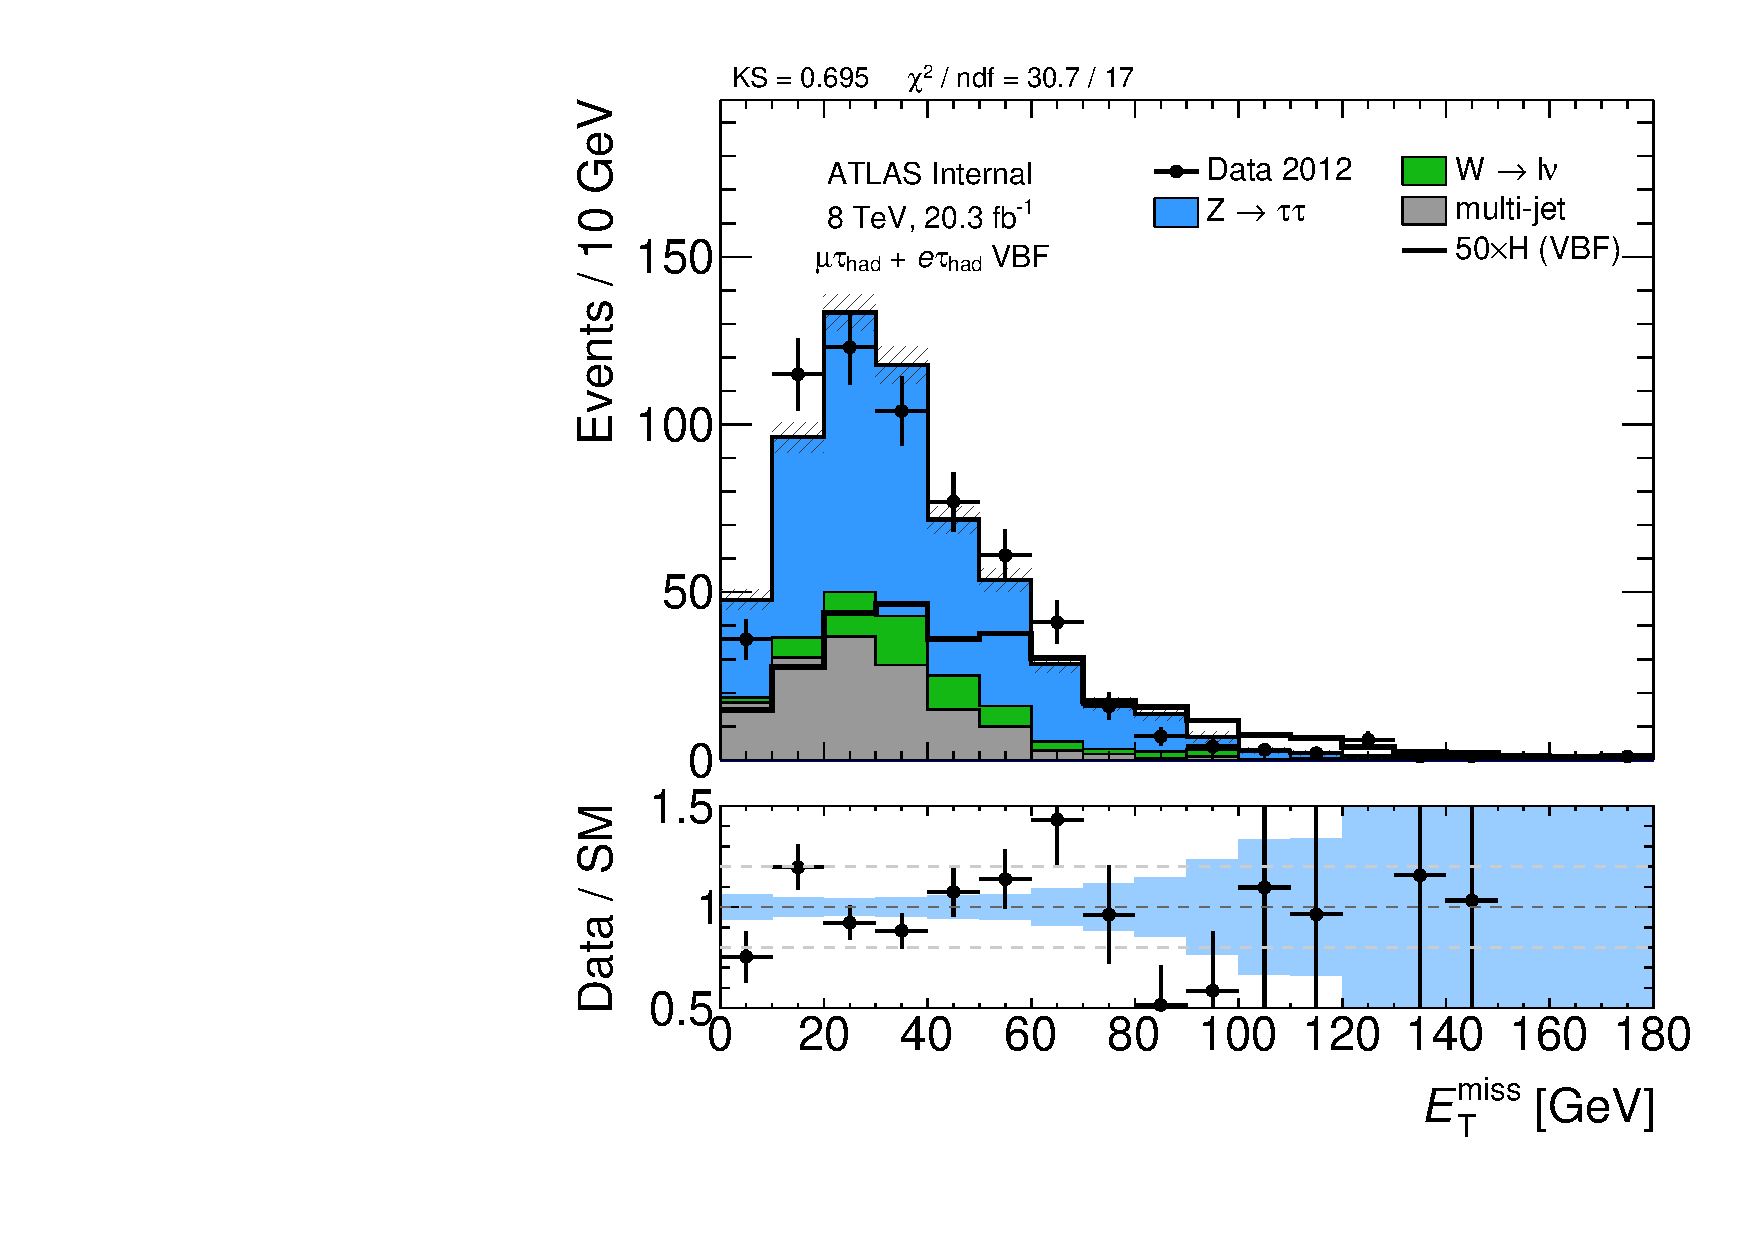
\includegraphics[width=0.32\textwidth]{figures/vbf-LTT/met-pt-hi}
  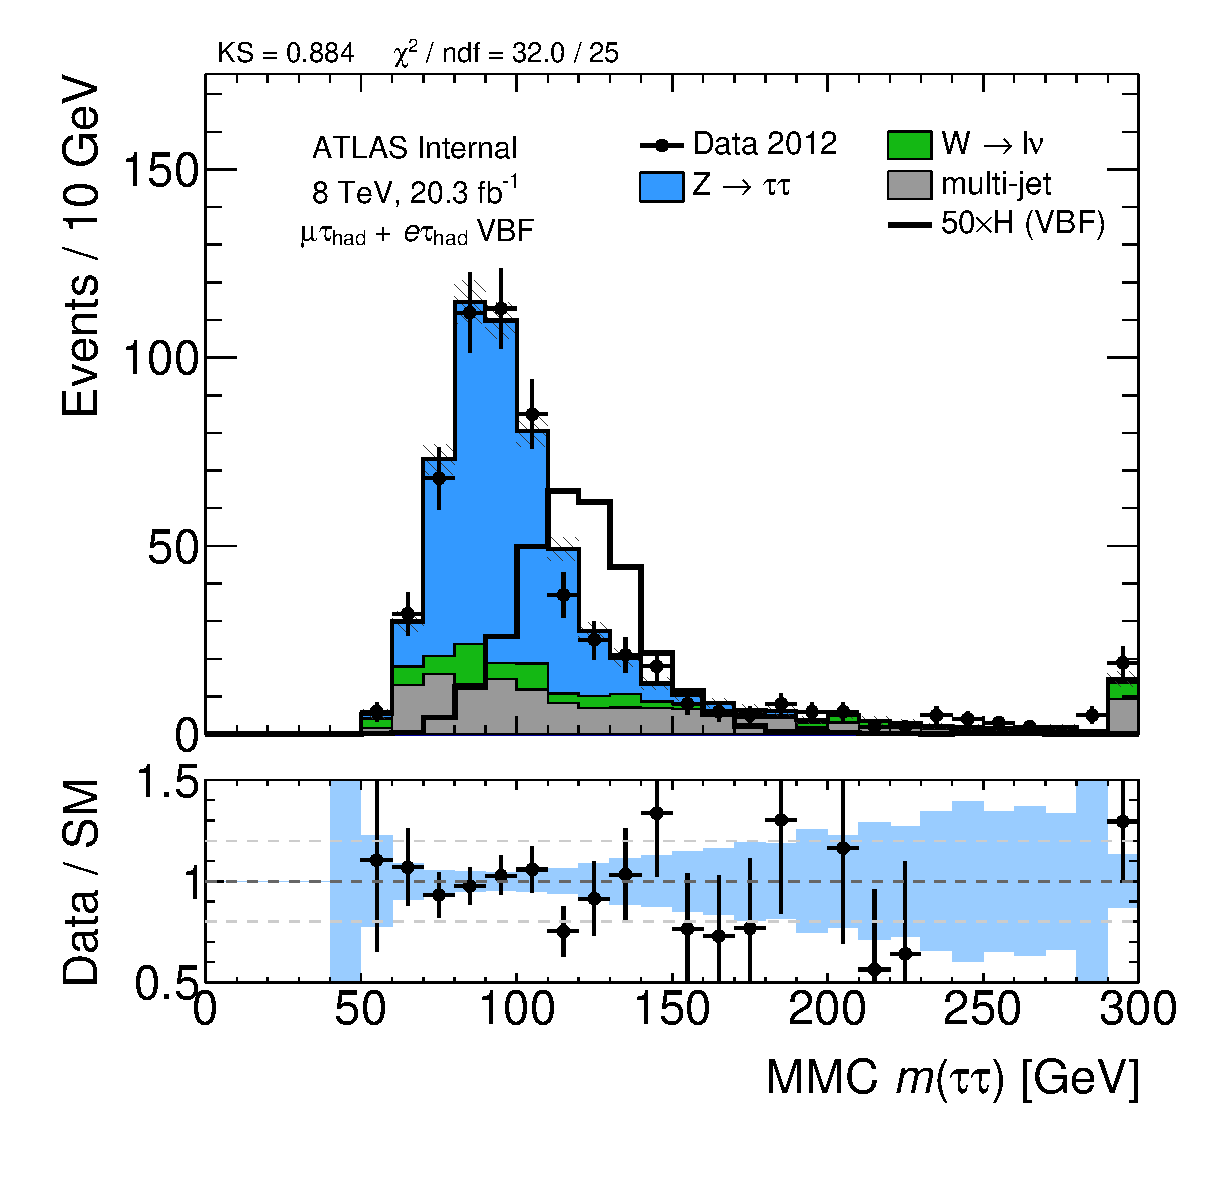
\includegraphics[width=0.32\textwidth]{figures/vbf-LTT/mMMC}
  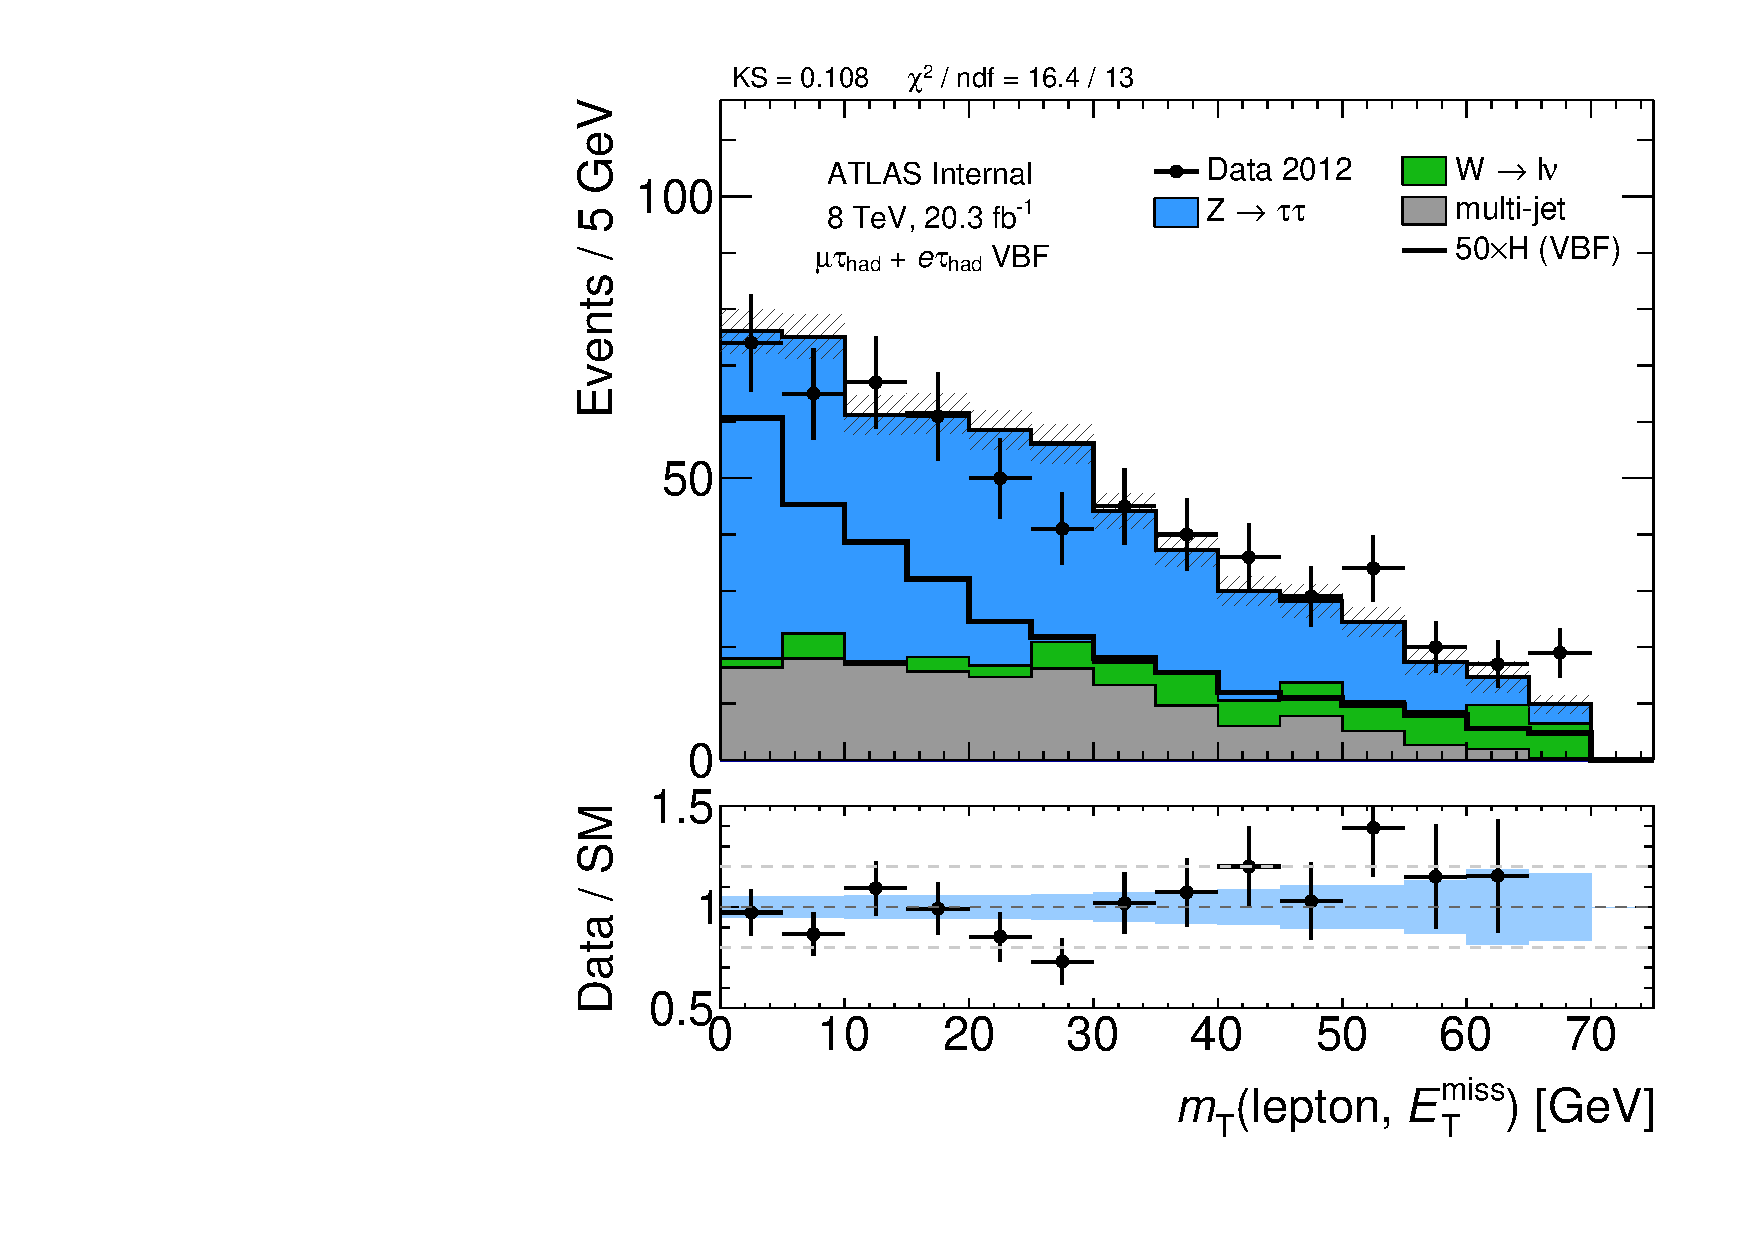
\includegraphics[width=0.32\textwidth]{figures/vbf-LTT/mT}
  % --------------
  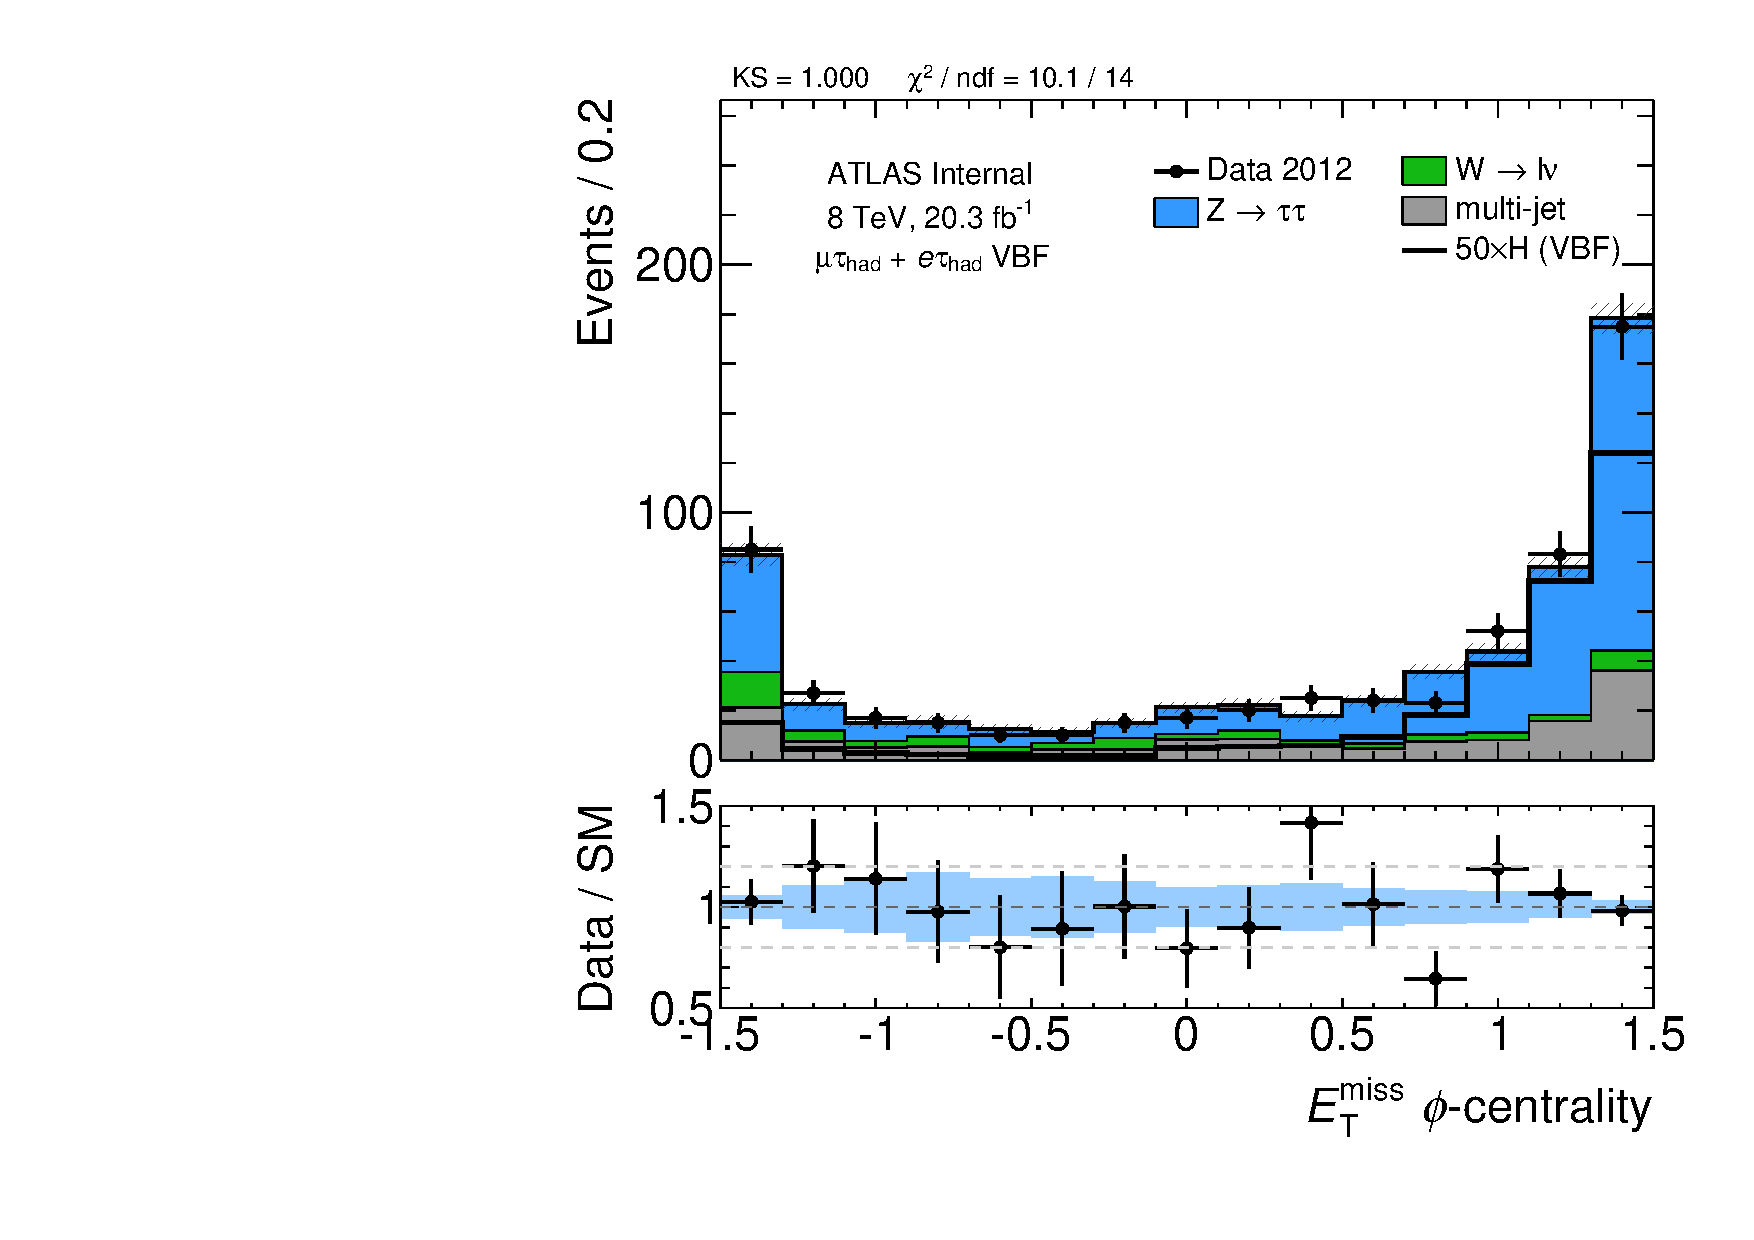
\includegraphics[width=0.32\textwidth]{figures/vbf-LTT/met-phi-centrality}
  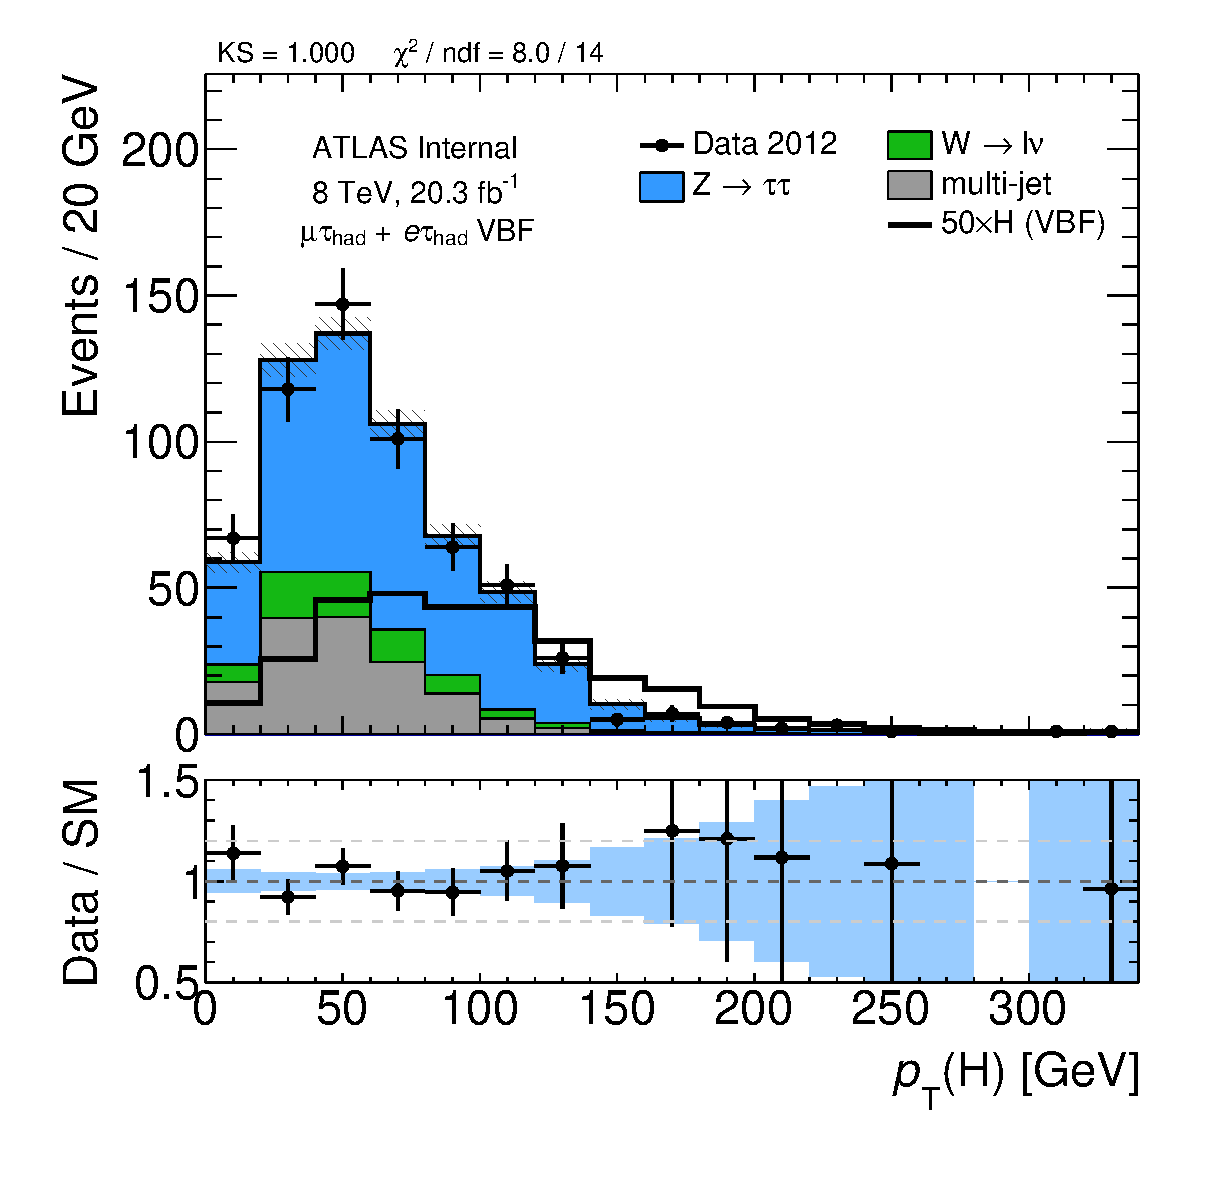
\includegraphics[width=0.32\textwidth]{figures/vbf-LTT/H-pt-hi}
  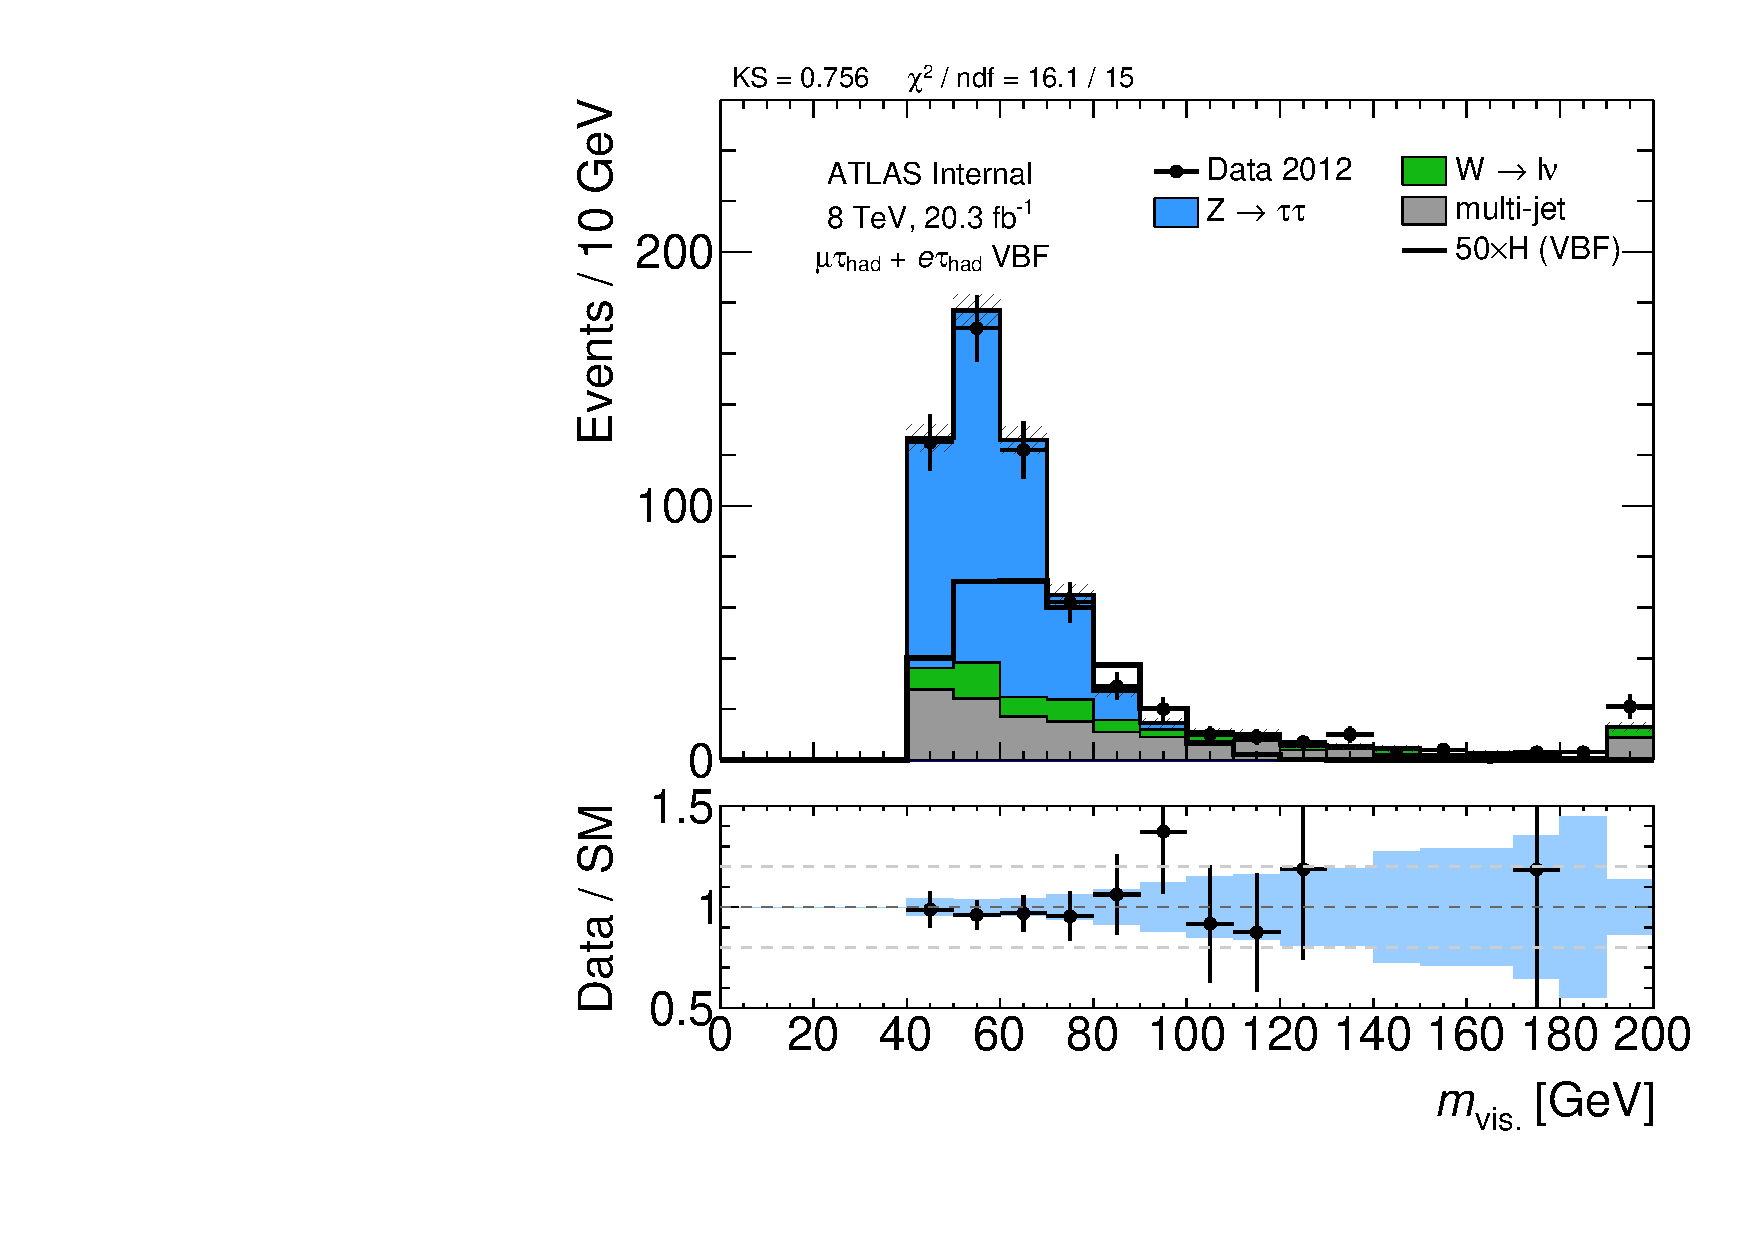
\includegraphics[width=0.32\textwidth]{figures/vbf-LTT/mvis}
  \caption{Kinematic distributions in the $\LTT$ category of the 8 TeV VBF $\Htautaulh$ analysis.}
  \label{fig:prospects-ltt-taus}
\end{figure}

\clearpage
\begin{figure}[tp]
  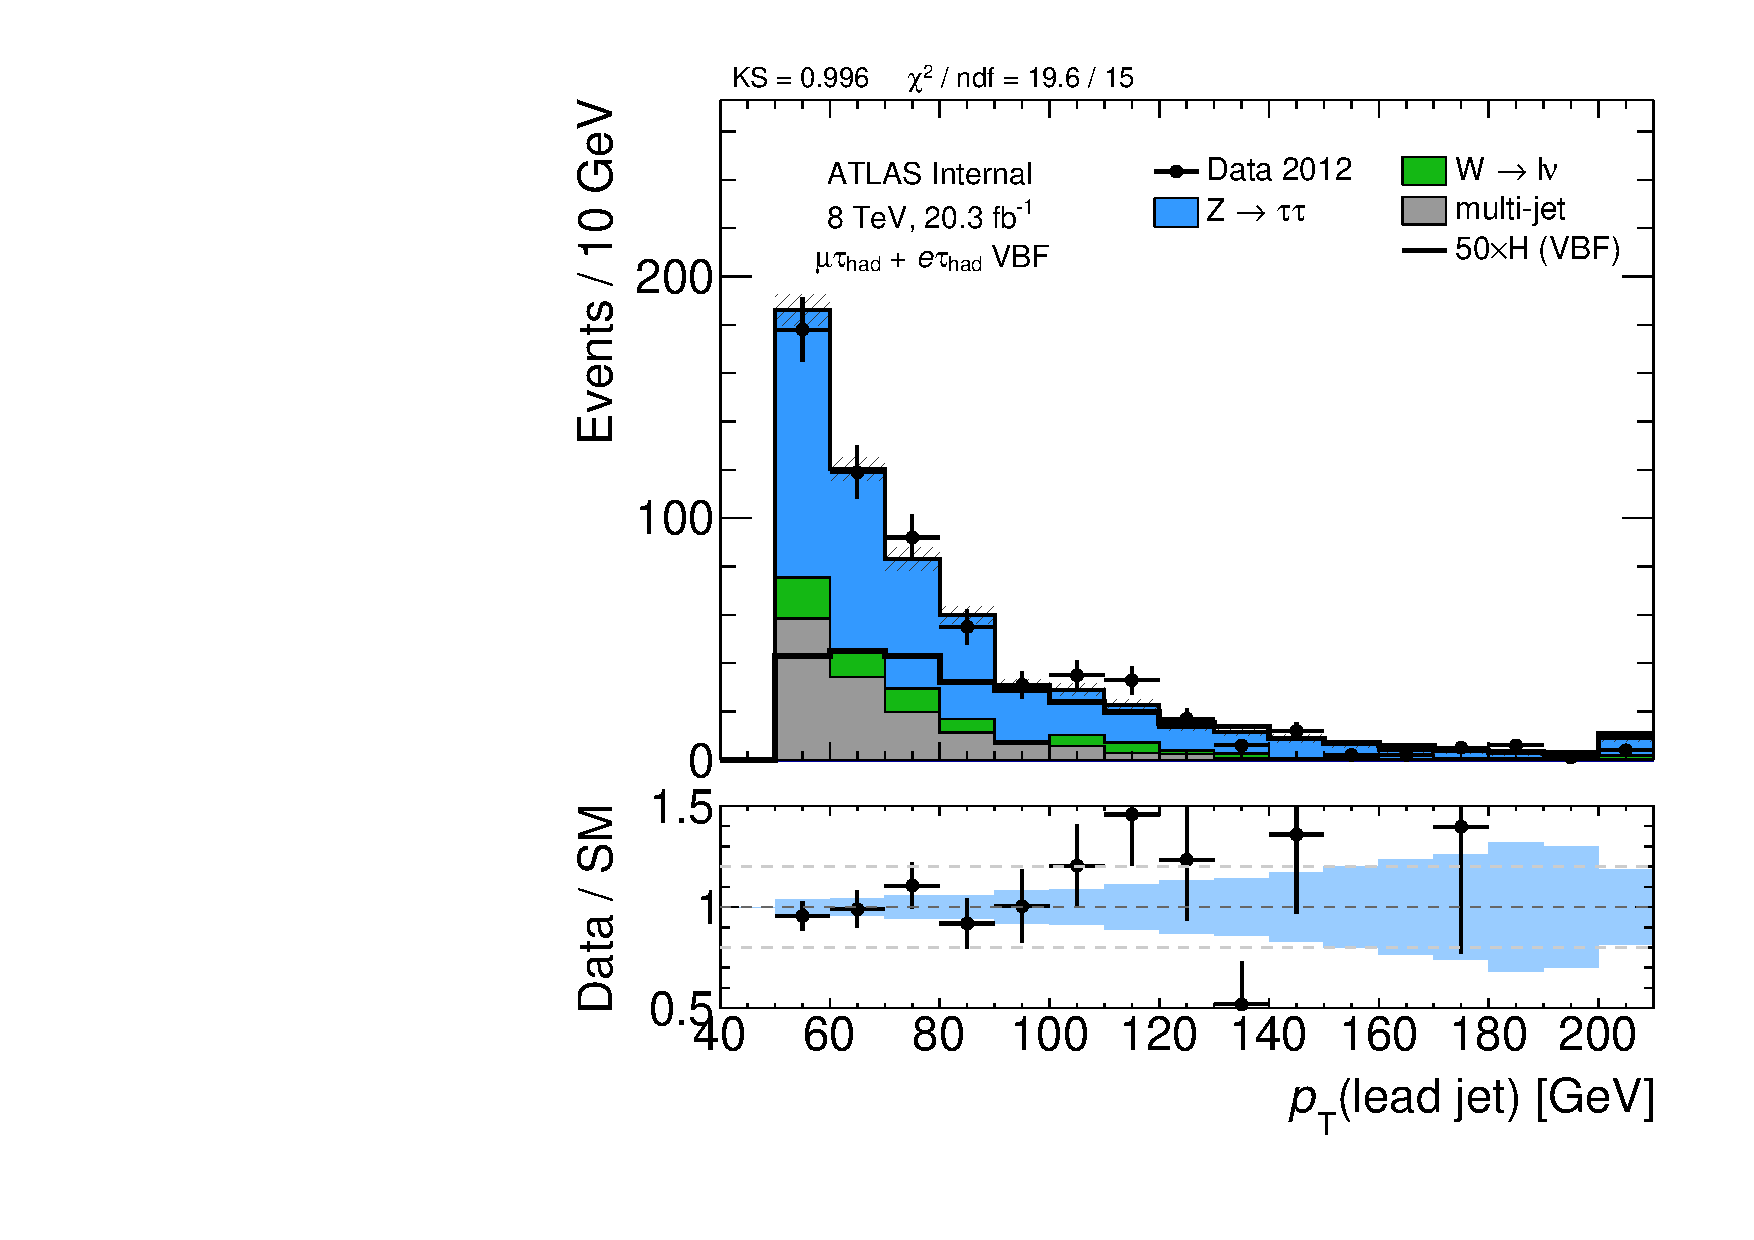
\includegraphics[width=0.32\textwidth]{figures/vbf-LTT/jet-1-pt}
  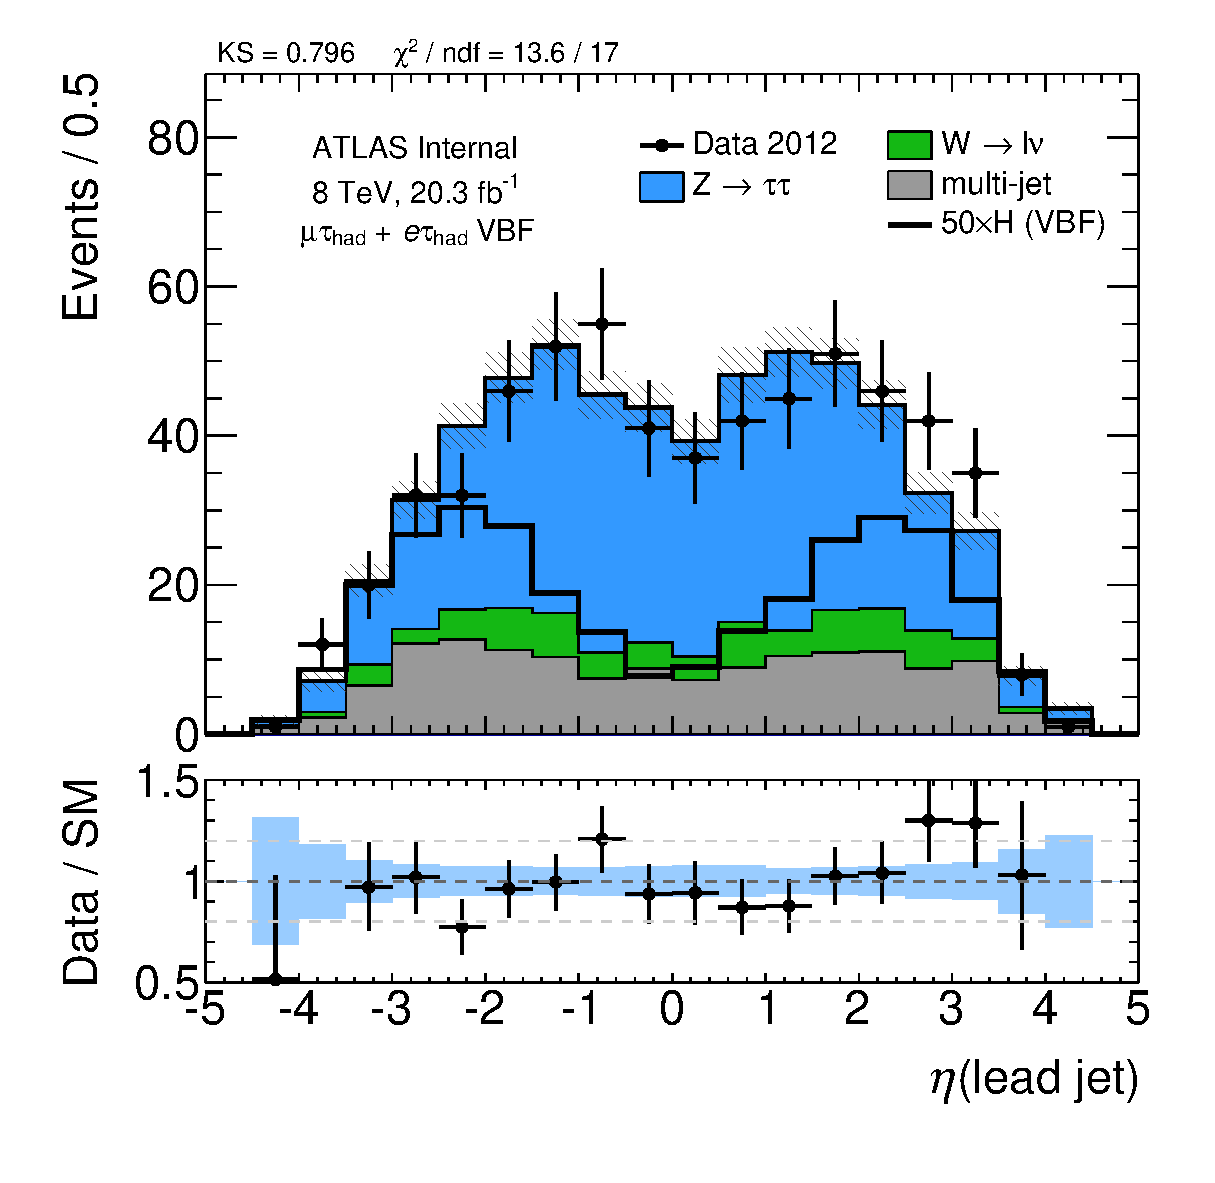
\includegraphics[width=0.32\textwidth]{figures/vbf-LTT/jet-1-eta}
  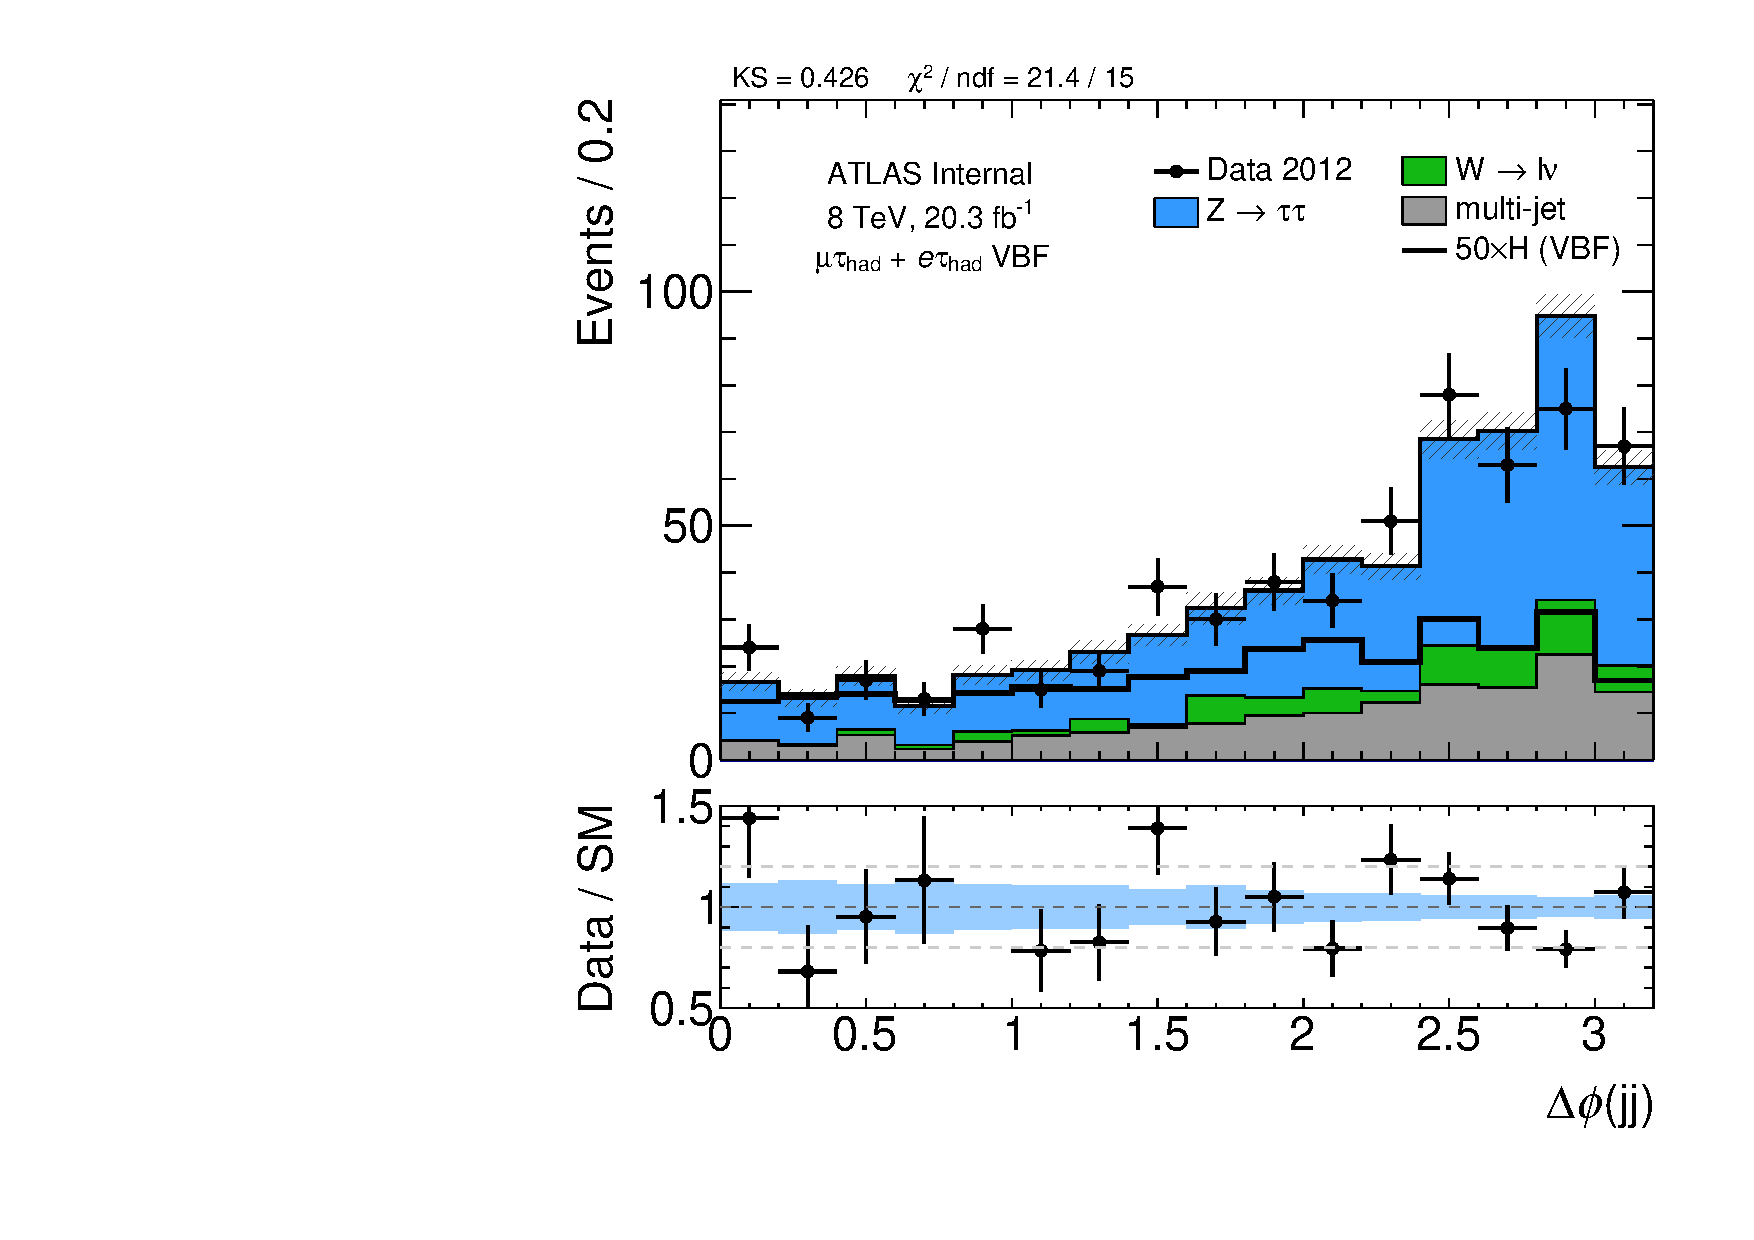
\includegraphics[width=0.32\textwidth]{figures/vbf-LTT/jets-dphi}
  % --------------
  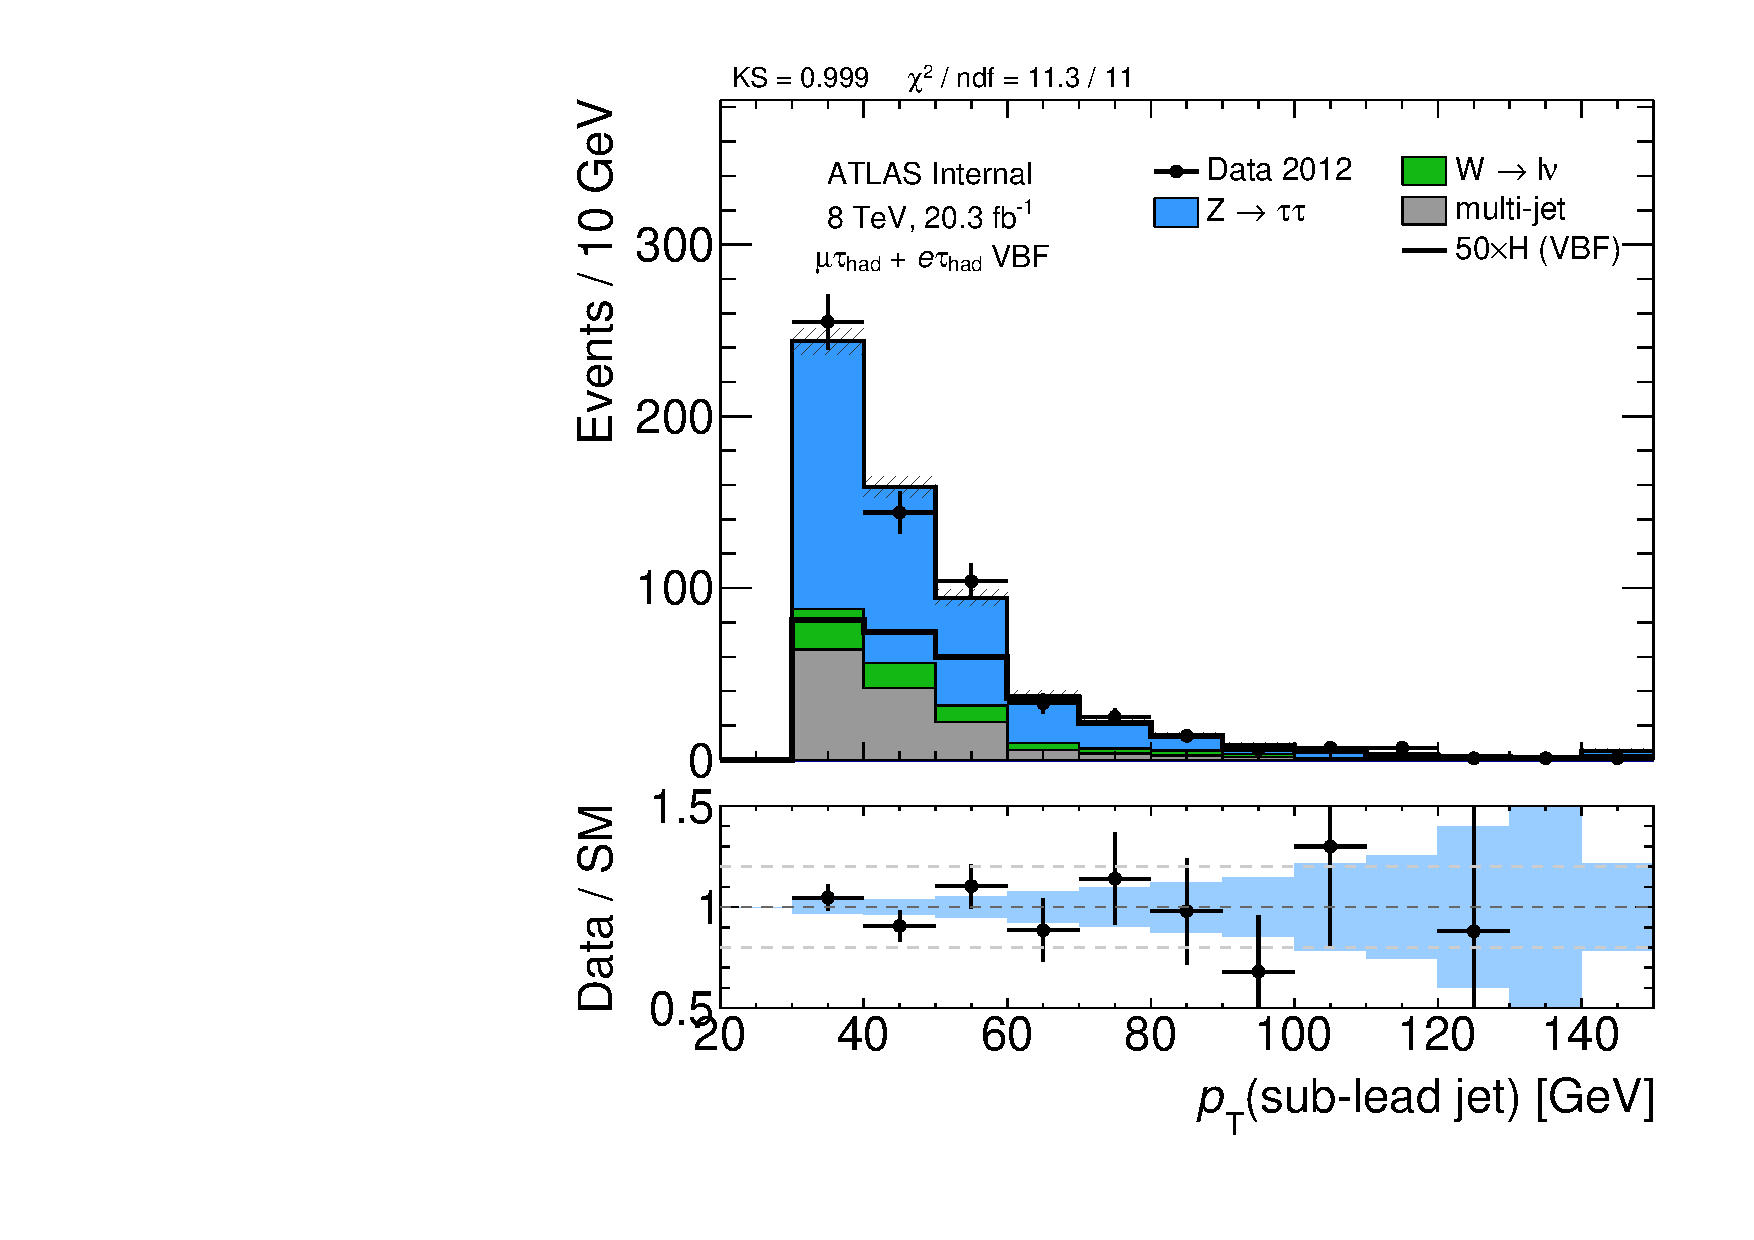
\includegraphics[width=0.32\textwidth]{figures/vbf-LTT/jet-2-pt}
  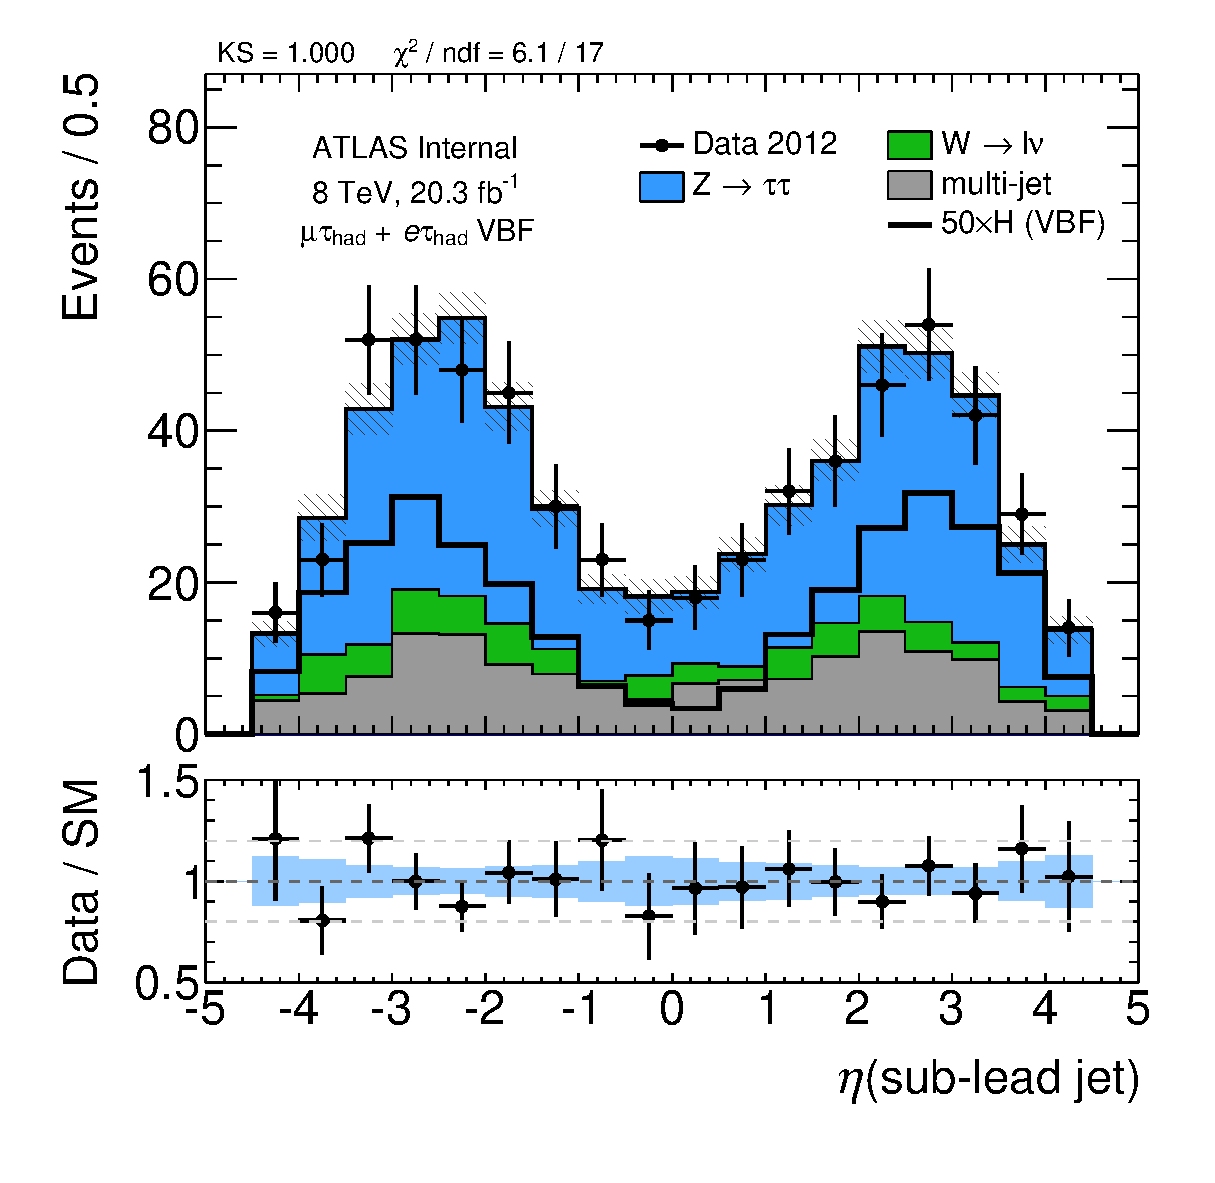
\includegraphics[width=0.32\textwidth]{figures/vbf-LTT/jet-2-eta}
  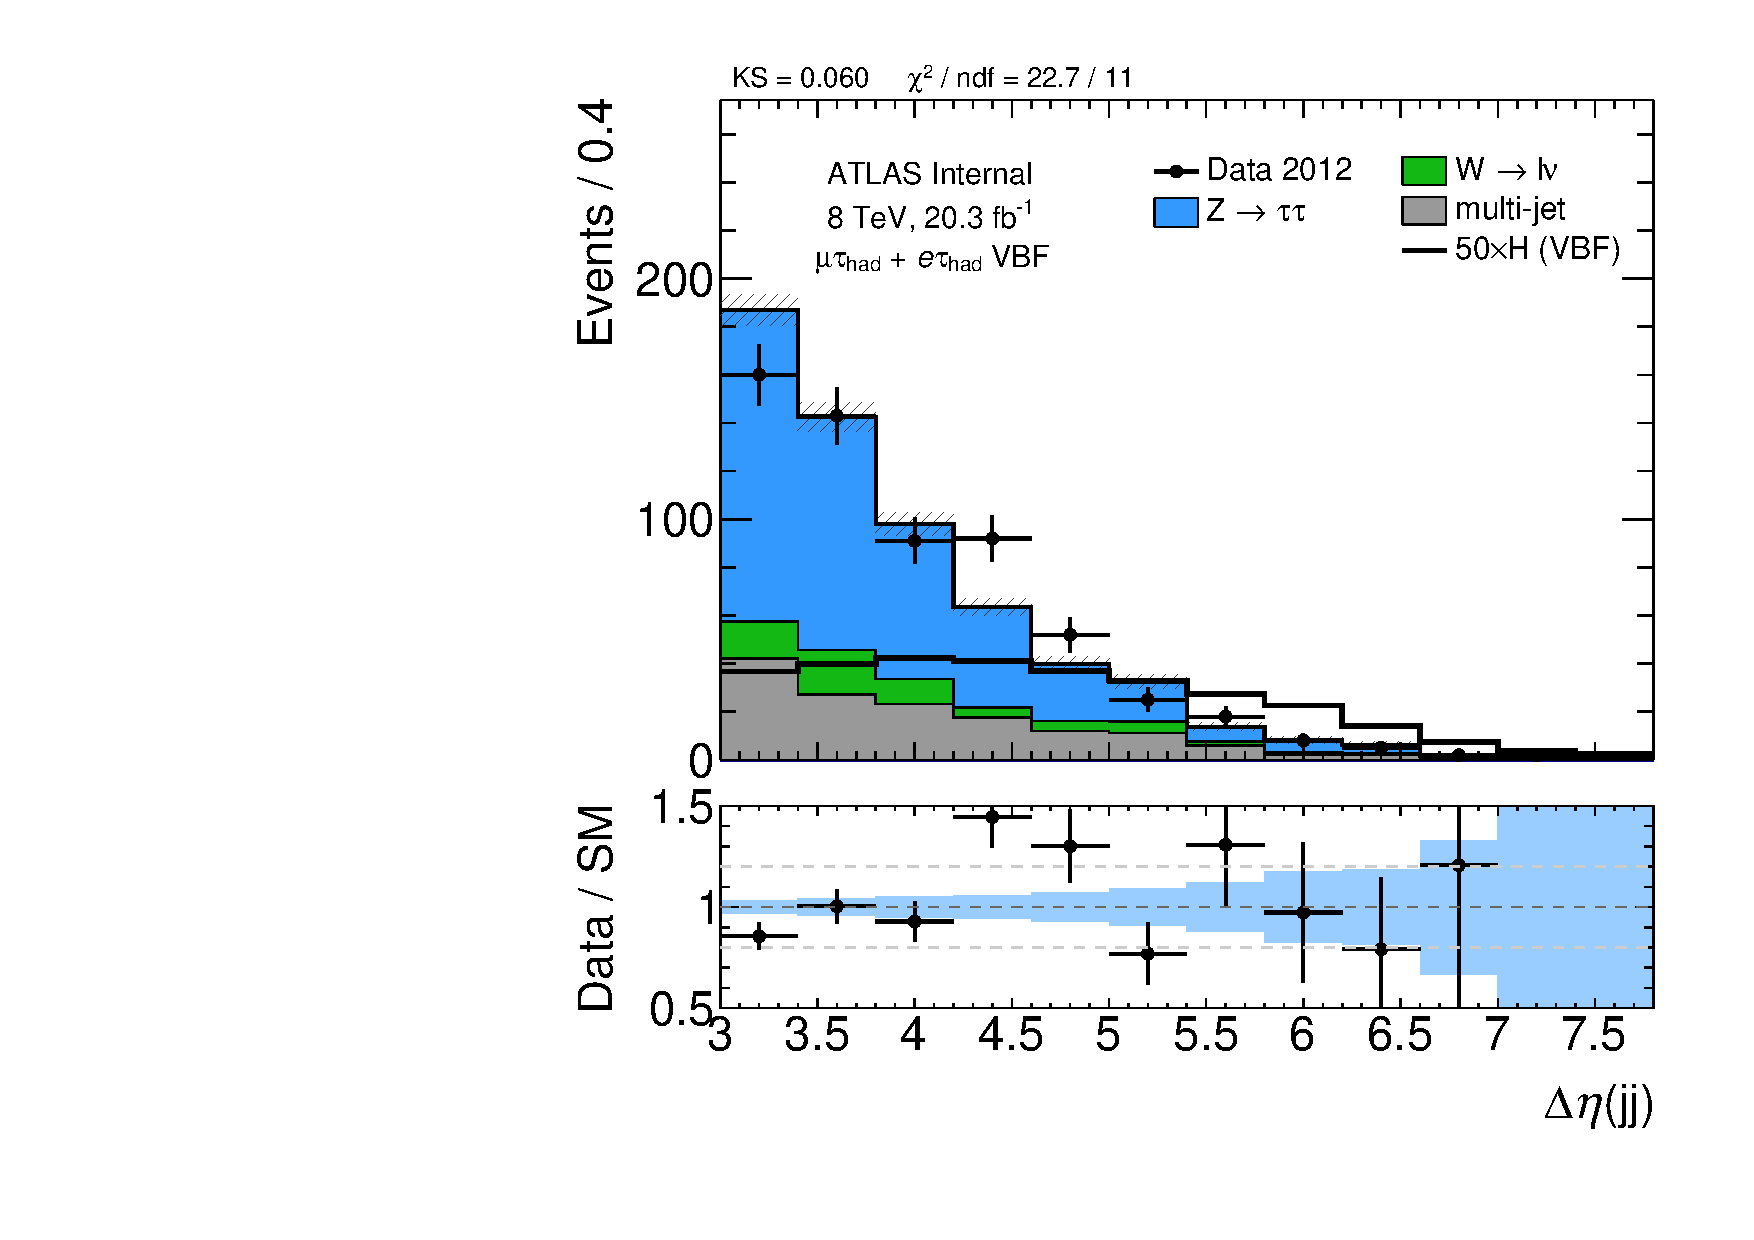
\includegraphics[width=0.32\textwidth]{figures/vbf-LTT/jets-deta}
  % --------------
  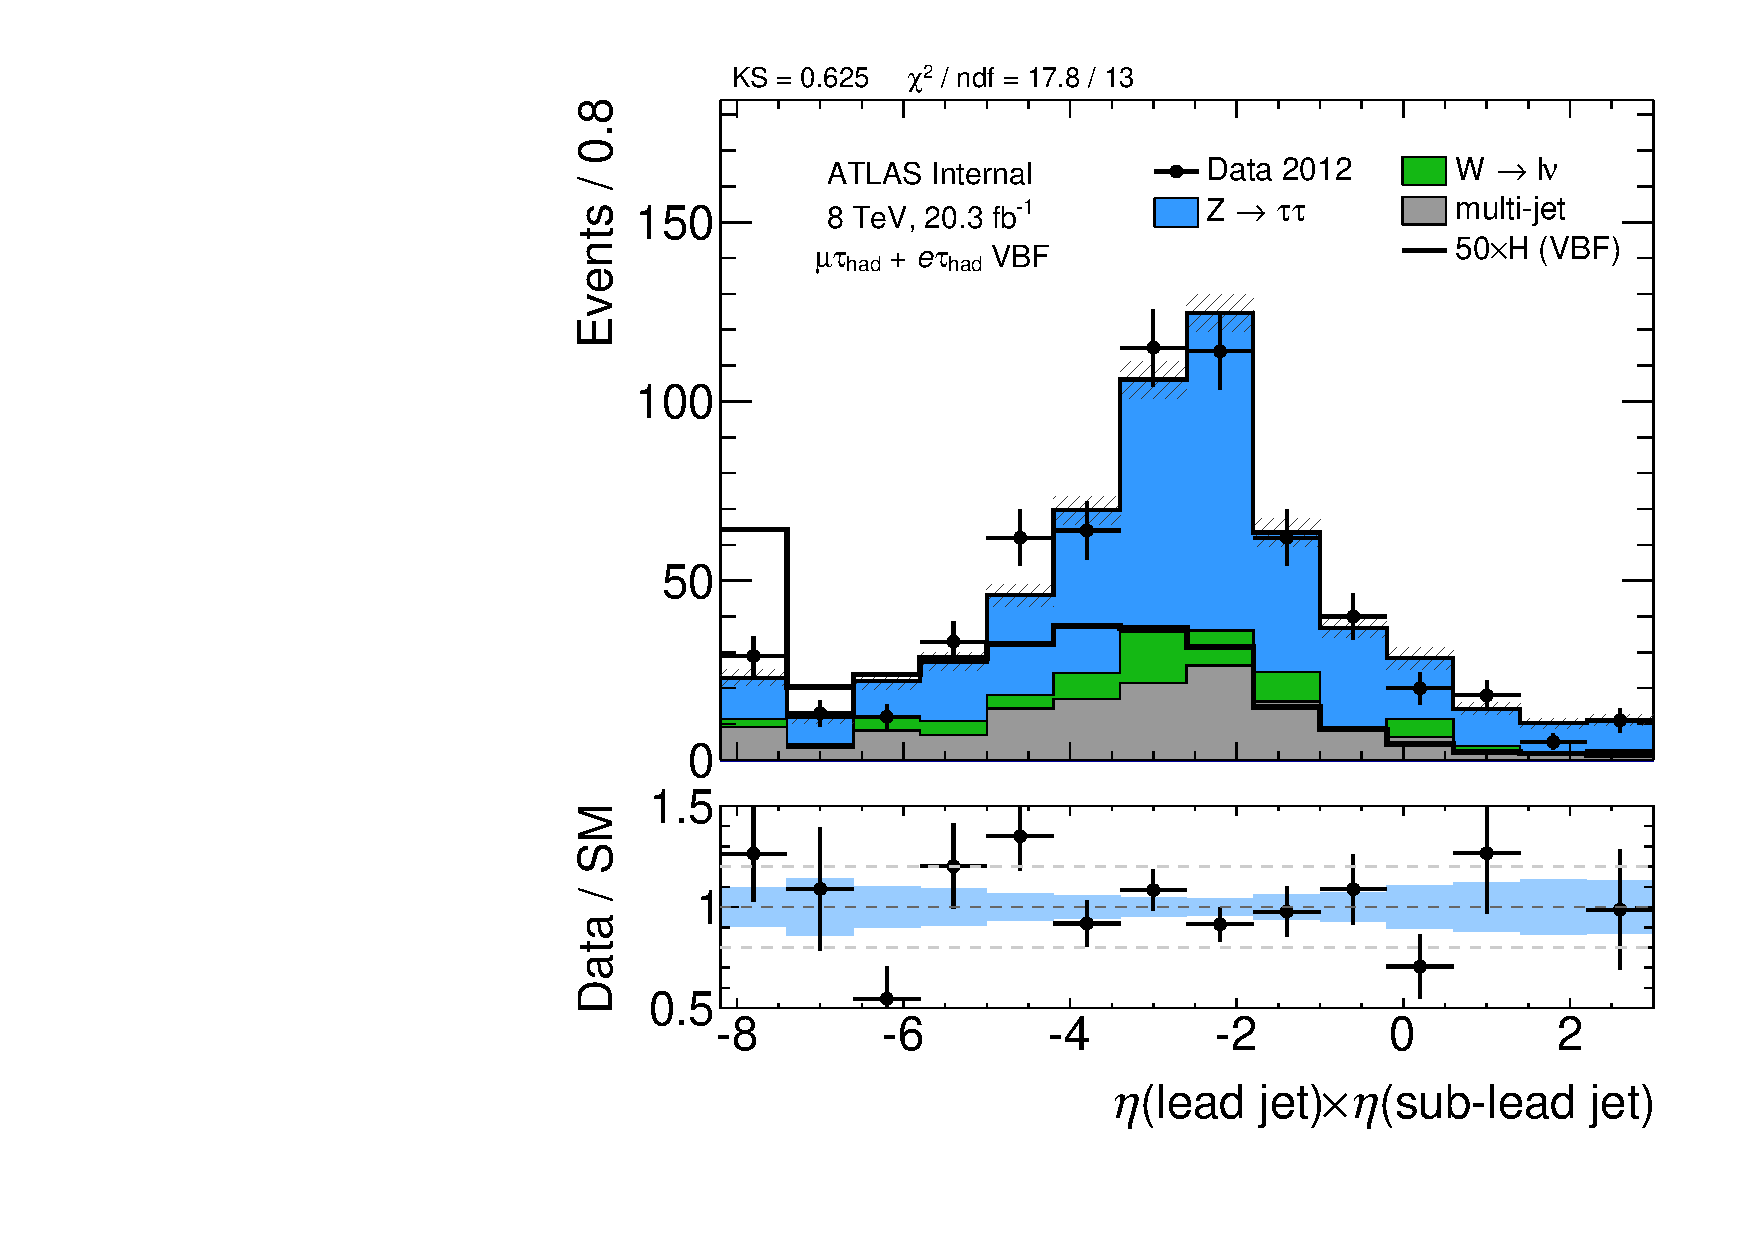
\includegraphics[width=0.32\textwidth]{figures/vbf-LTT/jets-etaprod}
  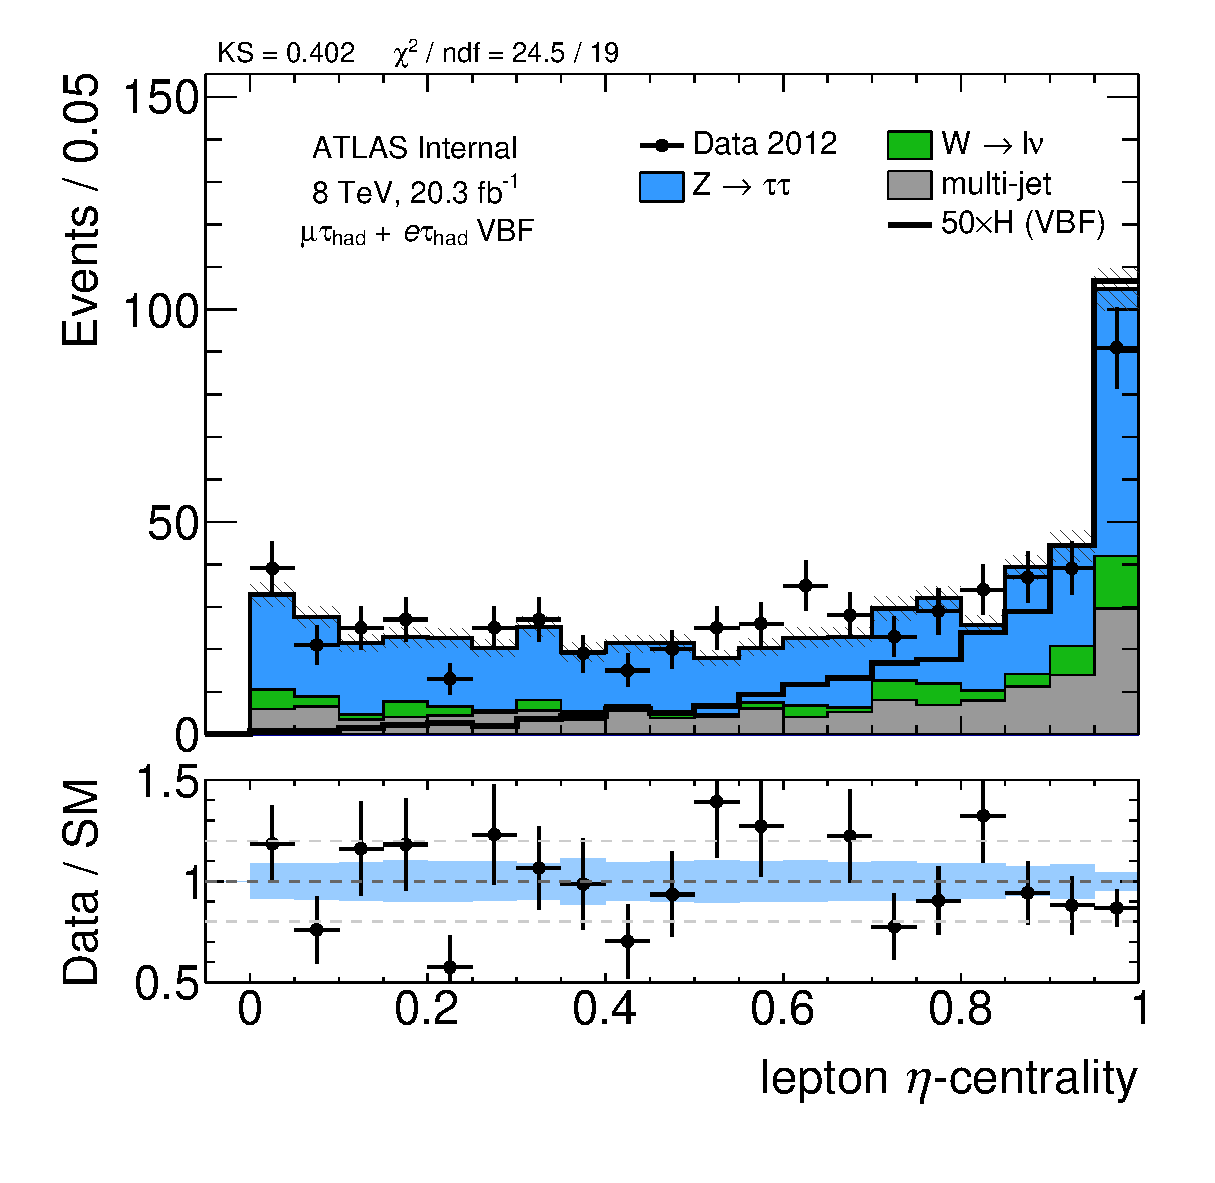
\includegraphics[width=0.32\textwidth]{figures/vbf-LTT/lep-eta-centrality}
  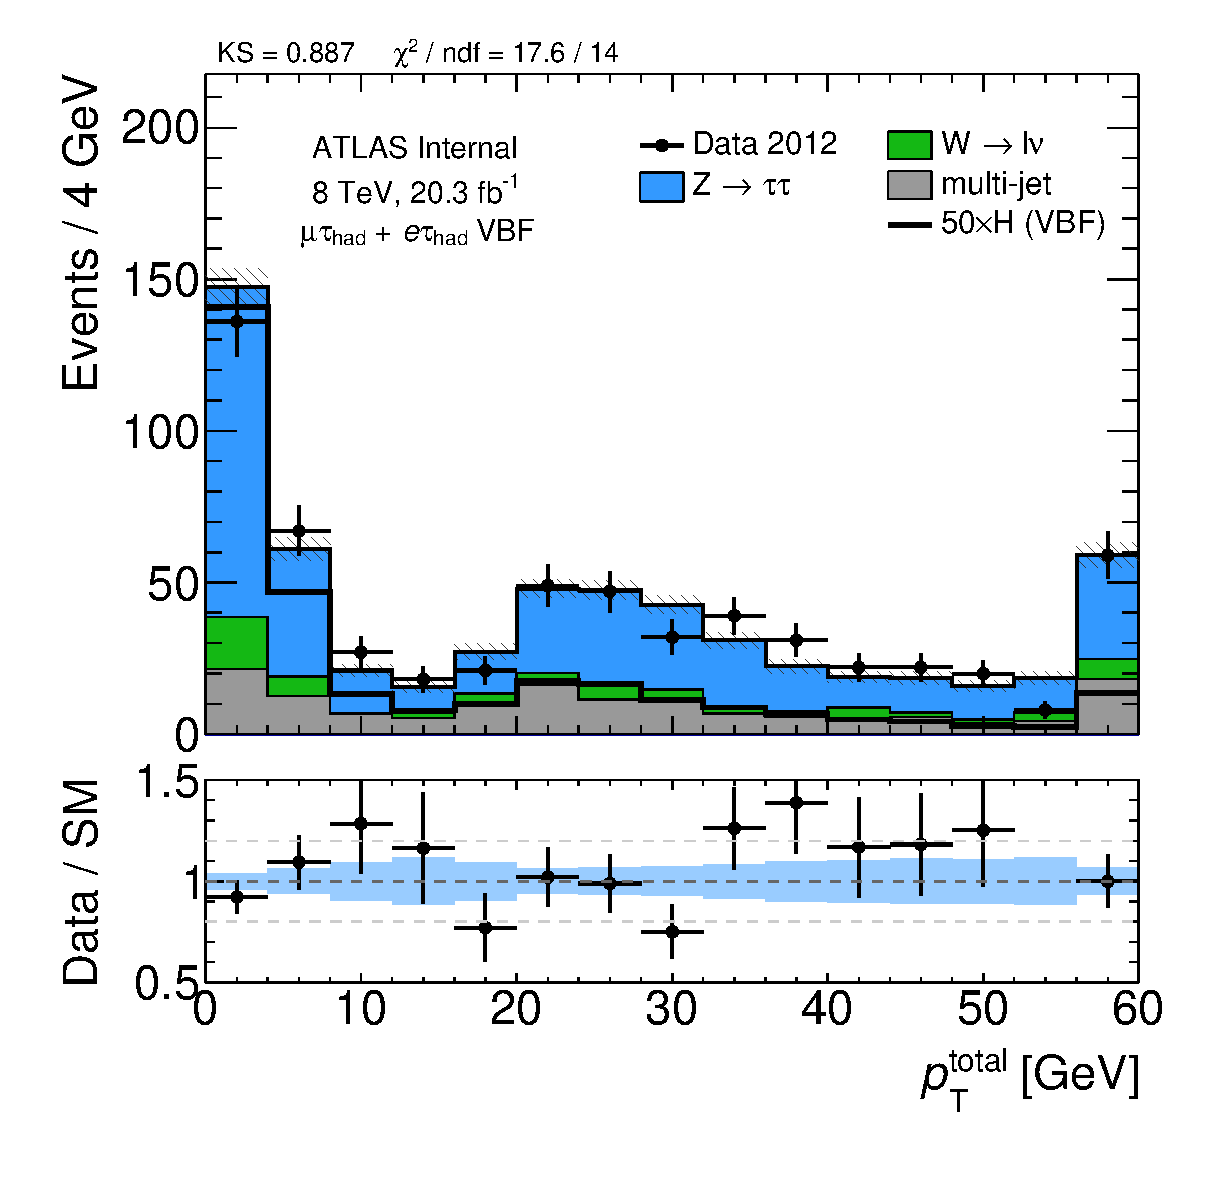
\includegraphics[width=0.32\textwidth]{figures/vbf-LTT/system-pt}
  % --------------
  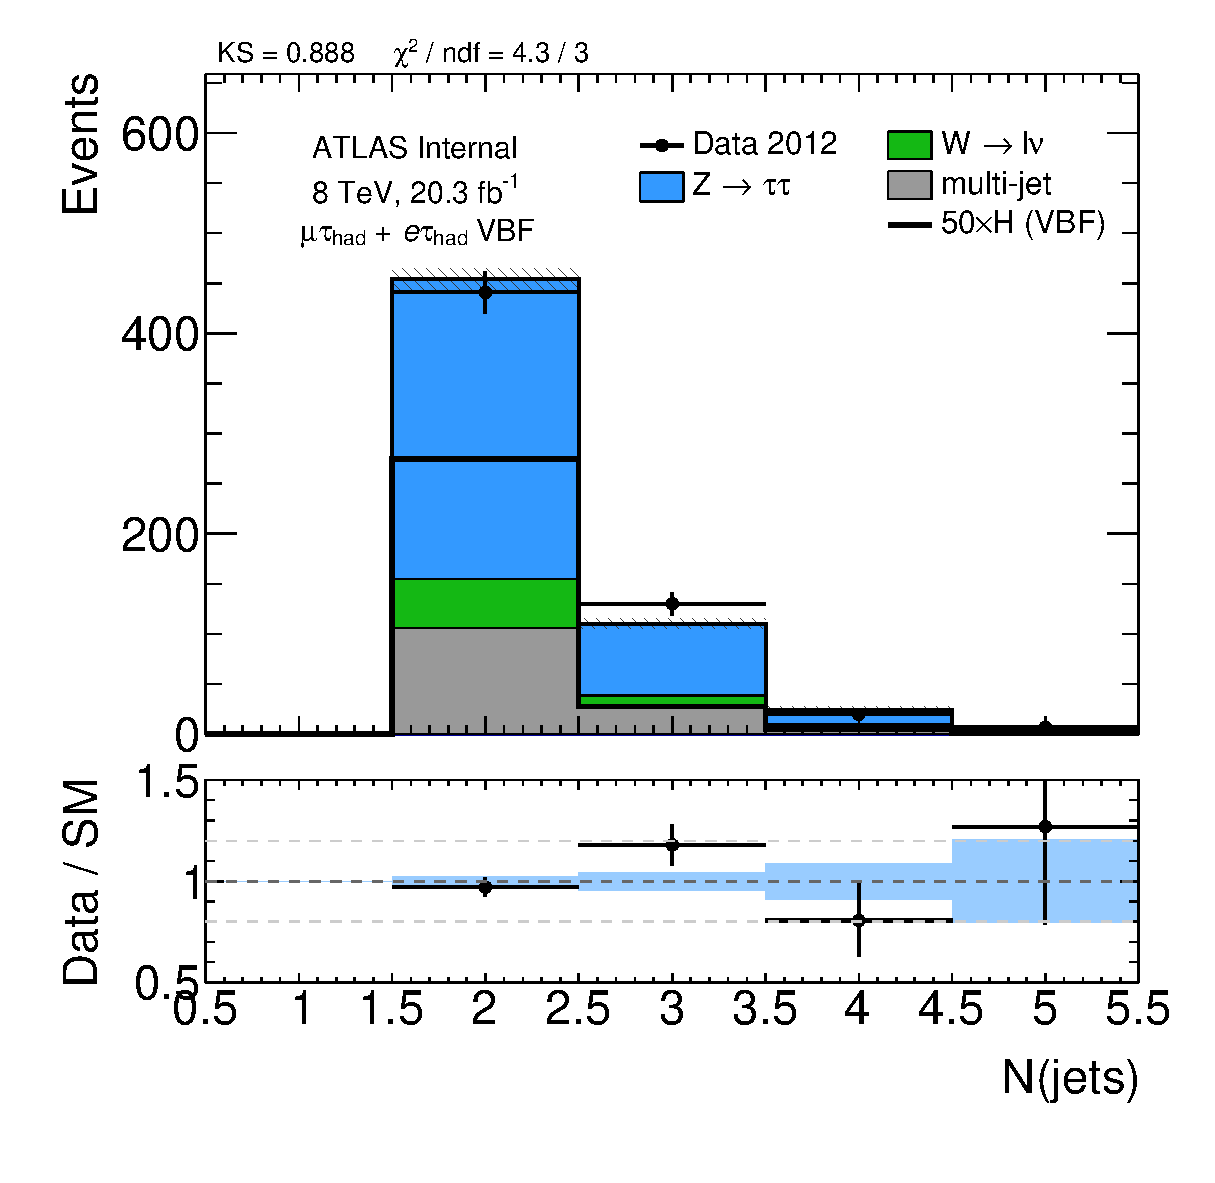
\includegraphics[width=0.32\textwidth]{figures/vbf-LTT/n-jets30}
  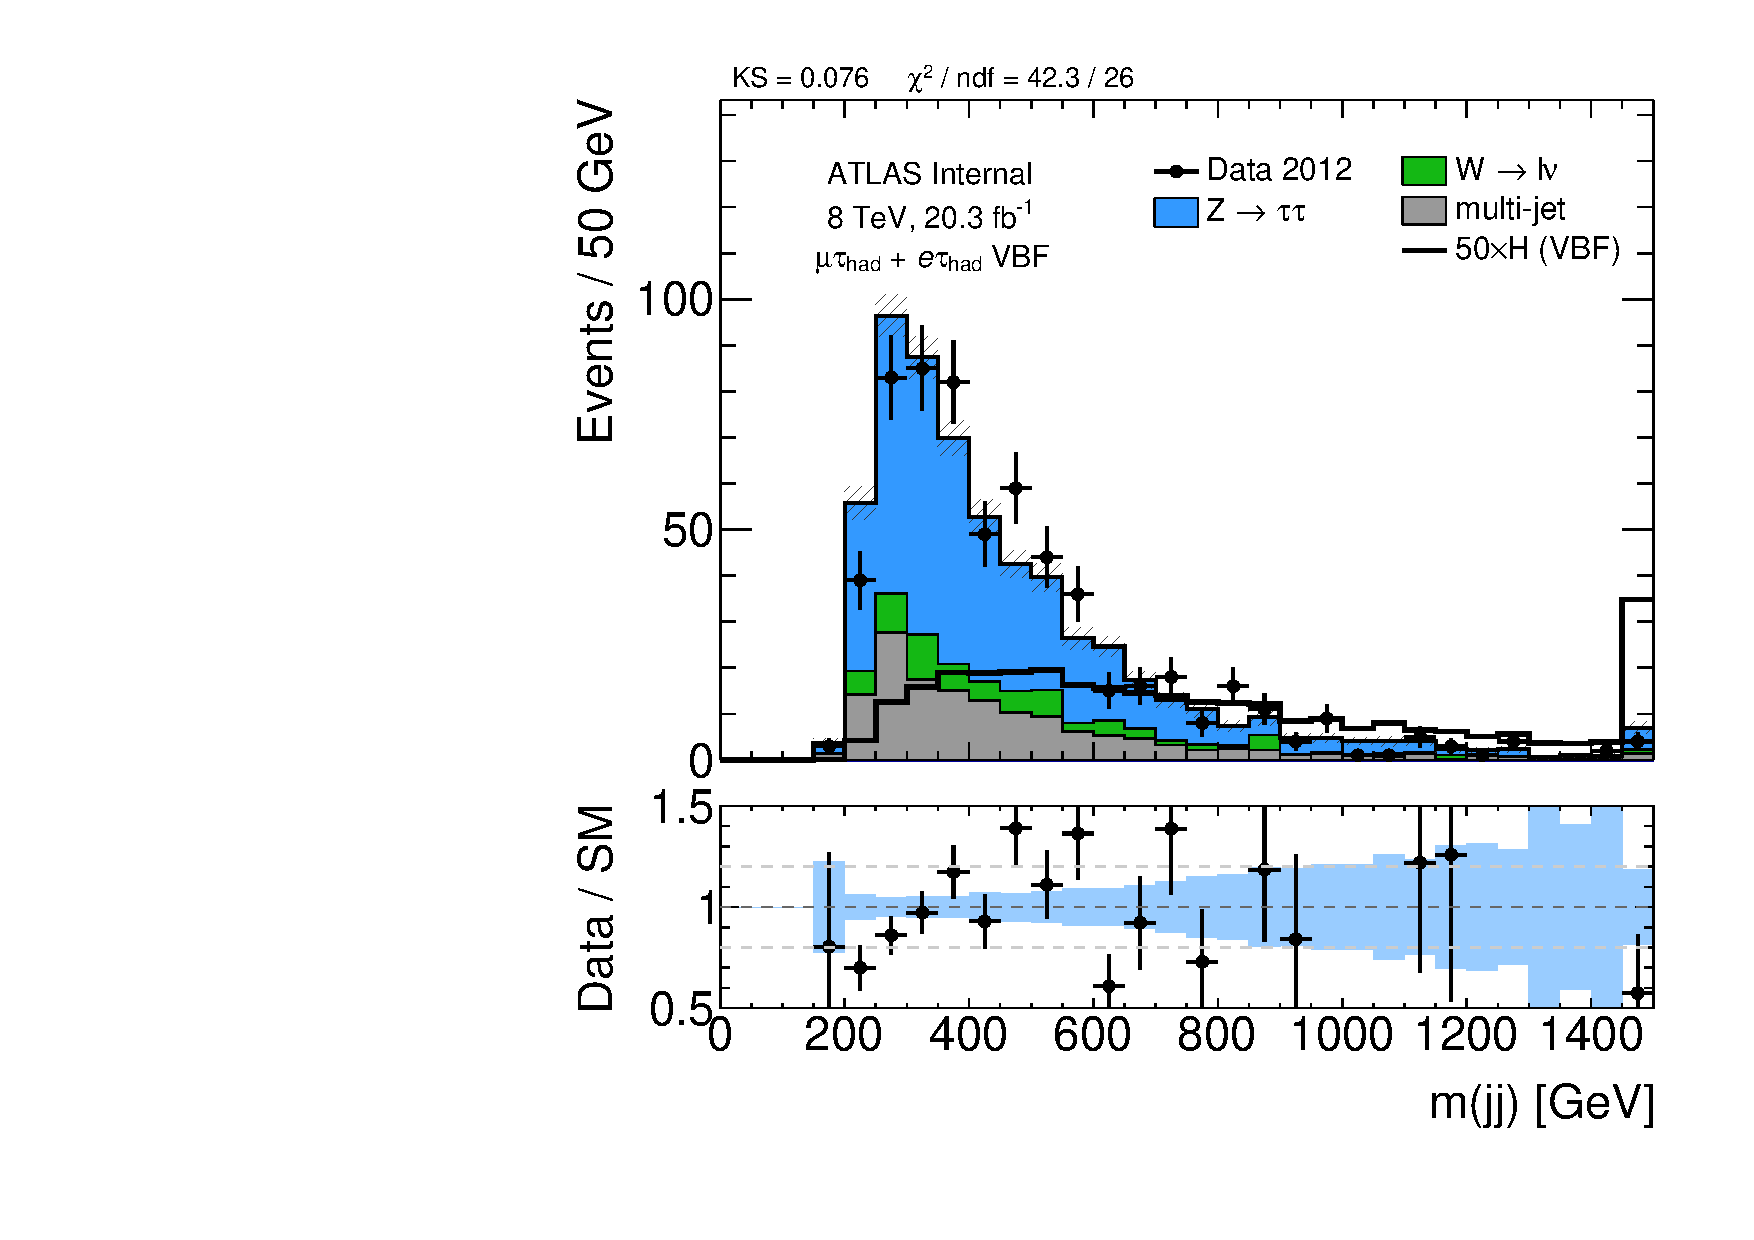
\includegraphics[width=0.32\textwidth]{figures/vbf-LTT/dijet-m-high}
  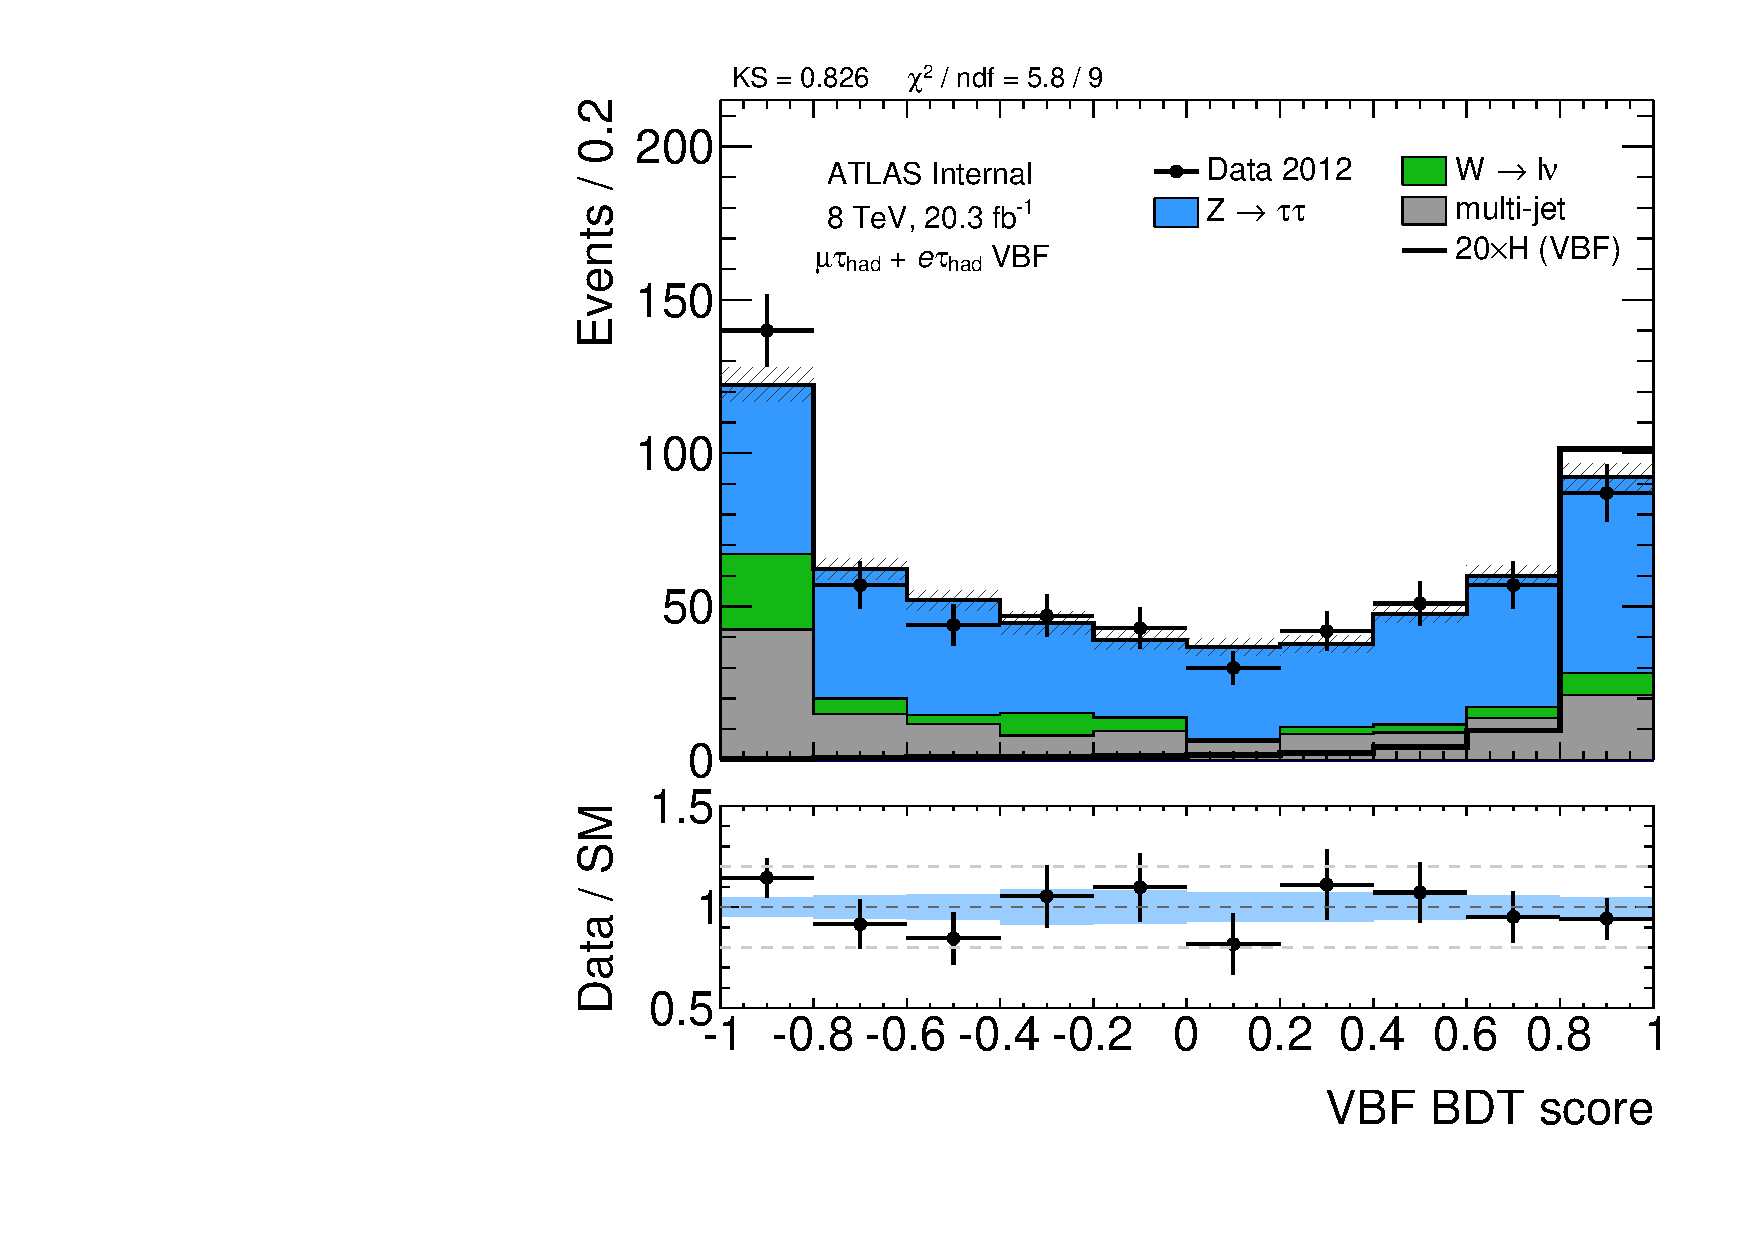
\includegraphics[width=0.32\textwidth]{figures/vbf-LTT/BDTEve-VBF}
  \caption{Kinematic distributions in the $\LTT$ category of the 8 TeV VBF $\Htautaulh$ analysis.}
  \label{fig:prospects-ltt-jets}
\end{figure}
\clearpage

\subsection{Updates to the L1 $\tauh$ object}

Updates to the L1 $\tauh$ object are also considered. 

\subsubsection{Size}

The size of the L1 $\tauh$ is made larger to check if a sharper efficiency turn-on curve can be gained without significant background contamination. This is especially important for 3-track $\tauh$, which are expected to be wider than 1-track $\tauh$ and are observed to have a slower efficiency turn-on curve. The default L1 $\tauh$ used in 2012 data-taking is $2 \times 1$ in the electromagnetic calorimeter and $2 \times 2$ in the hadronic calorimeter.

Efficiency turn-on curves for various L1 $\tauh$ definitions are shown in \cref{fig:prospects-trigger-towersize} for simulated $\tauh$ with and without isolation requirements. A sharper efficiency turn-on is achieved relative to the default definition, as shown in \cref{tab:prospects-tausize}. Since background rates increase non-trivially with larger L1 $\tauh$ objects, the default definition will be retained in 2015 data-taking.

\begin{figure}[!htpb]
  \centering
  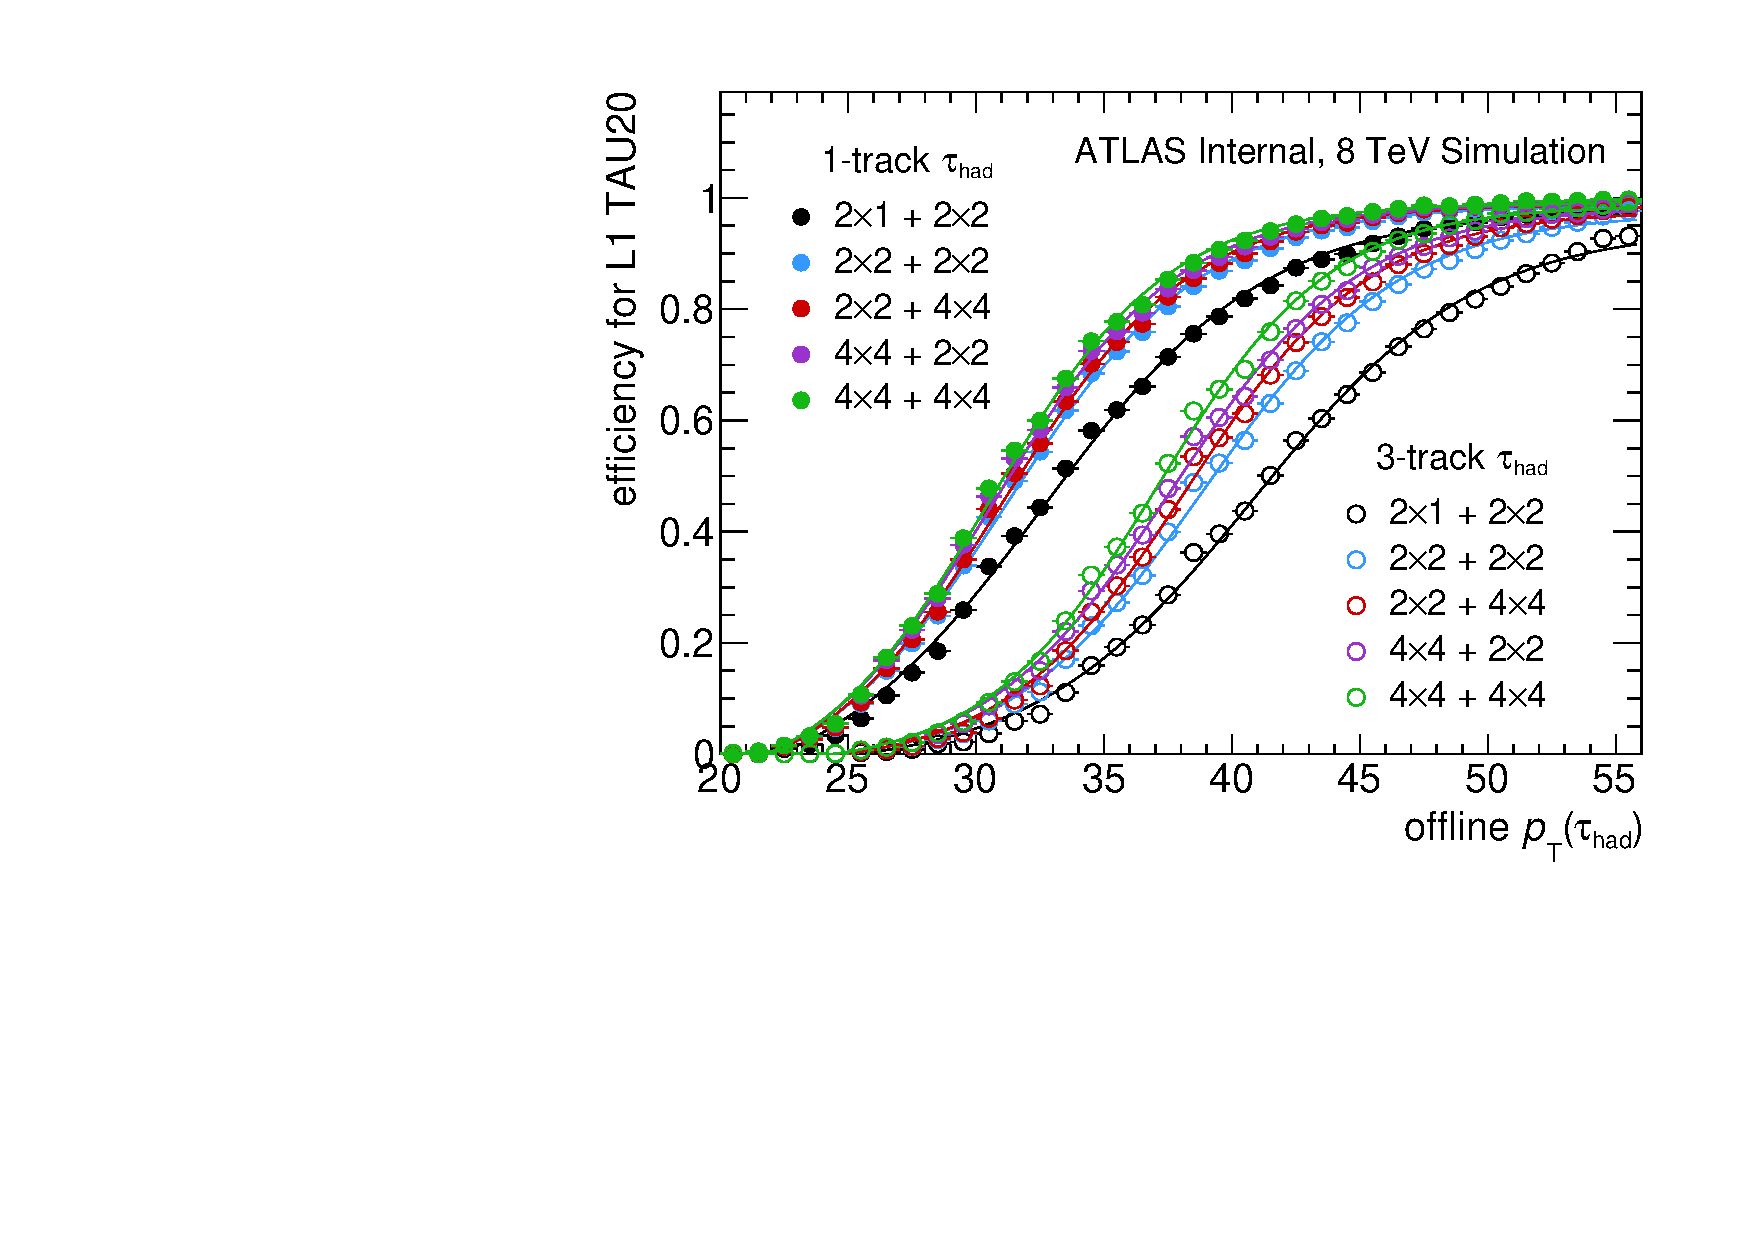
\includegraphics[width=0.48\textwidth]{figures/trigger/turnon_L1TAU20_1p3p}
  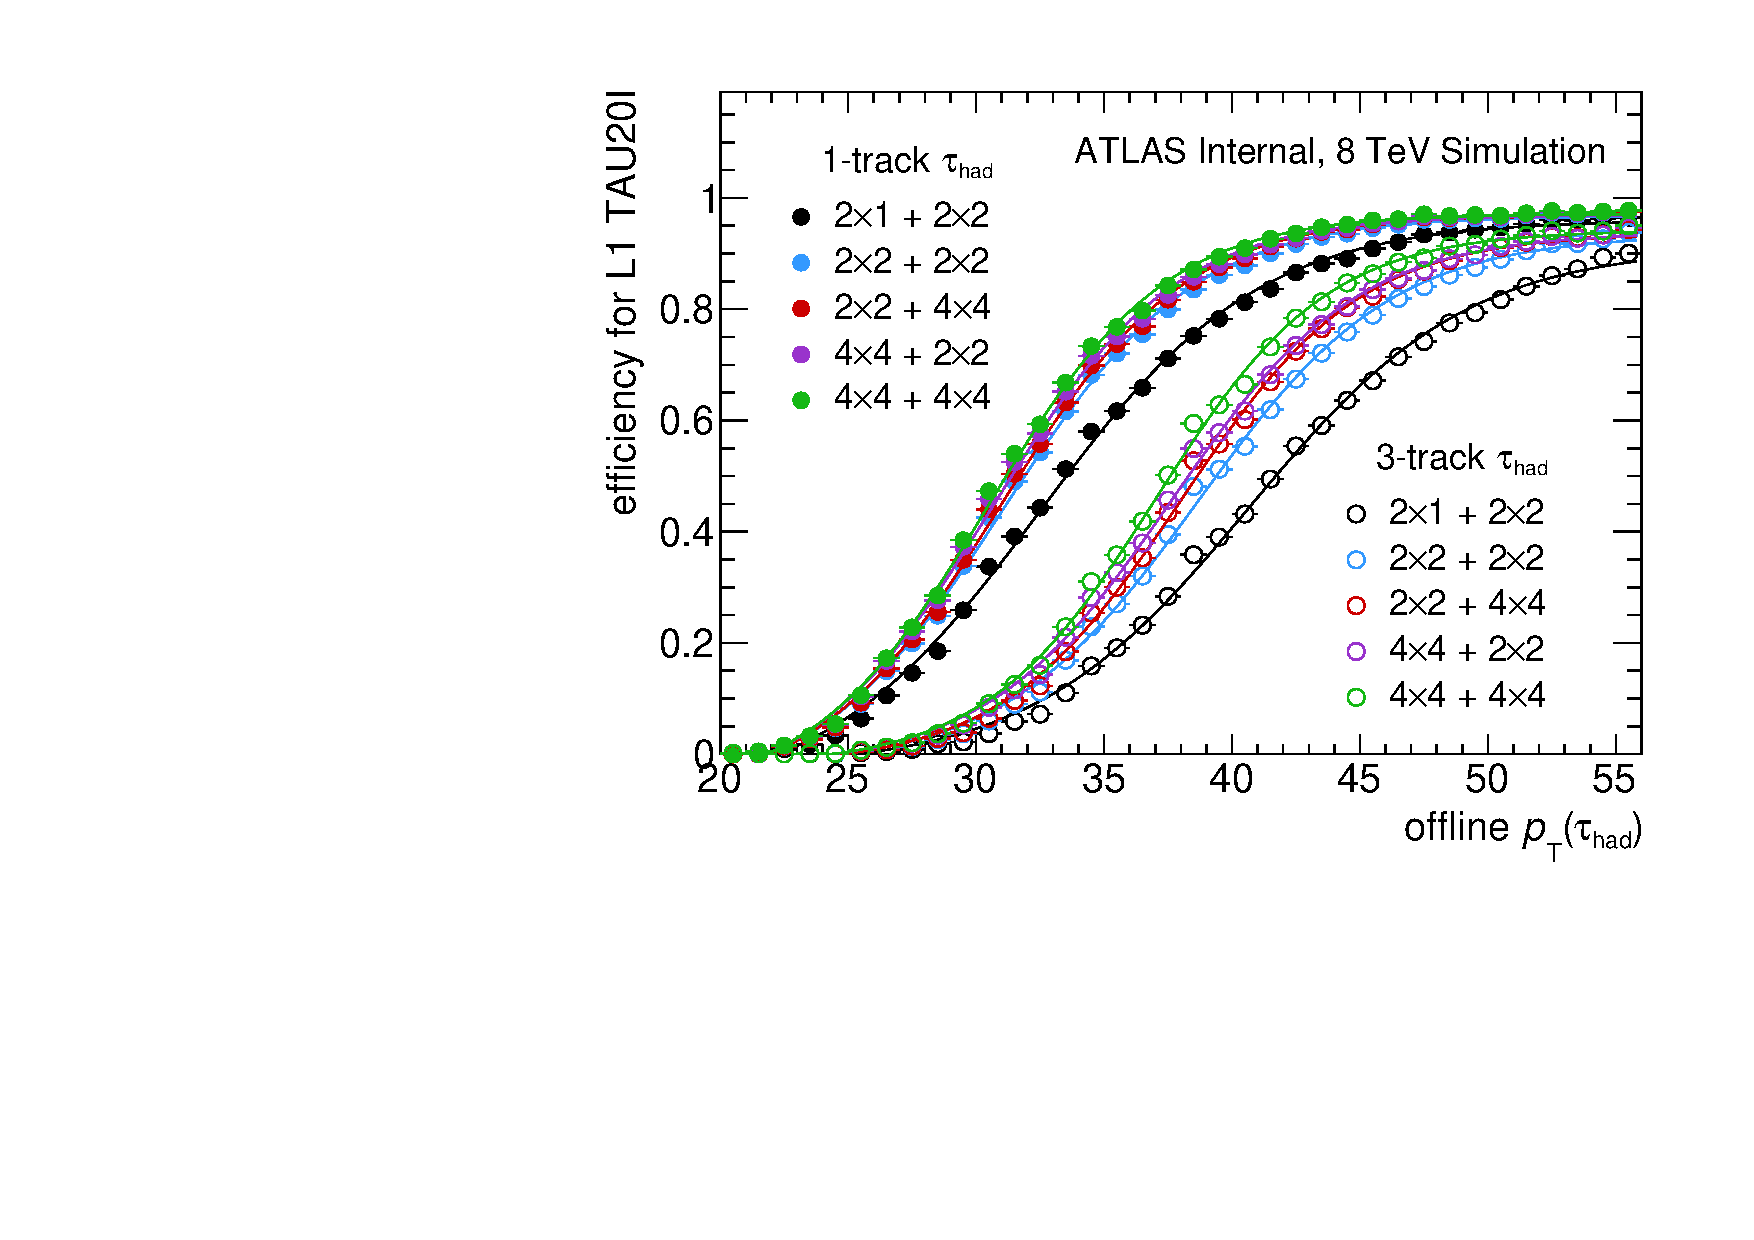
\includegraphics[width=0.48\textwidth]{figures/trigger/turnon_L1TAU20I_1p3p}
  \caption{Efficiency for firing the 20 GeV L1 $\tauh$ trigger as a function of offline $\pt(\tauh)$ for no isolation requirement (left) and the 2012 isolation requirement (right) for various definitions of the L1 $\tauh$ item. The current definition ($2 \times 1$ EM, $2 \times 2$ had.) has the slowest efficiency turn-on. Fits are performed with a Fermi-Dirac distribution.}
  \label{fig:prospects-trigger-towersize}
\end{figure}

\begin{table}[!htpb]
  \centering
  \renewcommand{\arraystretch}{1.4}
  \caption{Fits of the efficiency for firing the 20 GeV L1 $\tauh$ trigger with a Fermi-Dirac distribution for various definitions of the L1 $\tauh$ item. No isolation requirement is made.}
  \begin{tabular}{c|c|c|c}
  $\tauh$  & L1 size (EM, had.)                 & fitted $\pt$ offset [GeV] & fitted sharpness \\
  \hline\hline
           & $2 \!\times\! 1$, $2 \!\times\! 2$ & 32.6                      & 4.43             \\
           & $2 \!\times\! 2$, $2 \!\times\! 2$ & 31.2                      & 3.87             \\
  1-track  & $2 \!\times\! 2$, $4 \!\times\! 4$ & 31.0                      & 3.72             \\
           & $4 \!\times\! 4$, $2 \!\times\! 2$ & 30.7                      & 3.67             \\
           & $4 \!\times\! 4$, $4 \!\times\! 4$ & 30.5                      & 3.52             \\
  \hline
           & $2 \!\times\! 1$, $2 \!\times\! 2$ & 41.0                      & 4.47             \\
           & $2 \!\times\! 2$, $2 \!\times\! 2$ & 38.9                      & 3.93             \\
  3-track  & $2 \!\times\! 2$, $4 \!\times\! 4$ & 38.3                      & 3.65             \\
           & $4 \!\times\! 4$, $2 \!\times\! 2$ & 37.7                      & 3.71             \\
           & $4 \!\times\! 4$, $4 \!\times\! 4$ & 37.1                      & 3.42             \\
\end{tabular}

  \label{tab:prospects-tausize}
\end{table}

\clearpage

\subsubsection{Isolation}

The definition of L1 isolation is also reconsidered for 2015 data-taking. In 2012, a flat cut of $\pt^\text{L1,iso} \leq 4$ GeV is used. In 2015, the option of $\pt^\text{L1}$-dependent isolation is available. A simple linear dependence is explored:
%
\begin{equation}
  \begin{split}
    \text{require} \ \pt^\text{L1,iso} &\leq m \times \pt^\text{L1,iso} + b \ \text{GeV} \\
   \end{split}
  \label{eqn:prospects-L1iso}
\end{equation}
%
With the definition, the 2012 isolation requirement is $m=0$ and $b=4$.

Removing the isolation requirement is considered above $\pt^\text{L1} = 60$ GeV. This is equivalent to a logical \texttt{OR} with the lowest unprescaled single $\tauh$ trigger, \texttt{TAU60}, and thus will not cost any additional unique rate to the total L1 trigger menu.

\begin{figure}[!htpb]
  \centering
  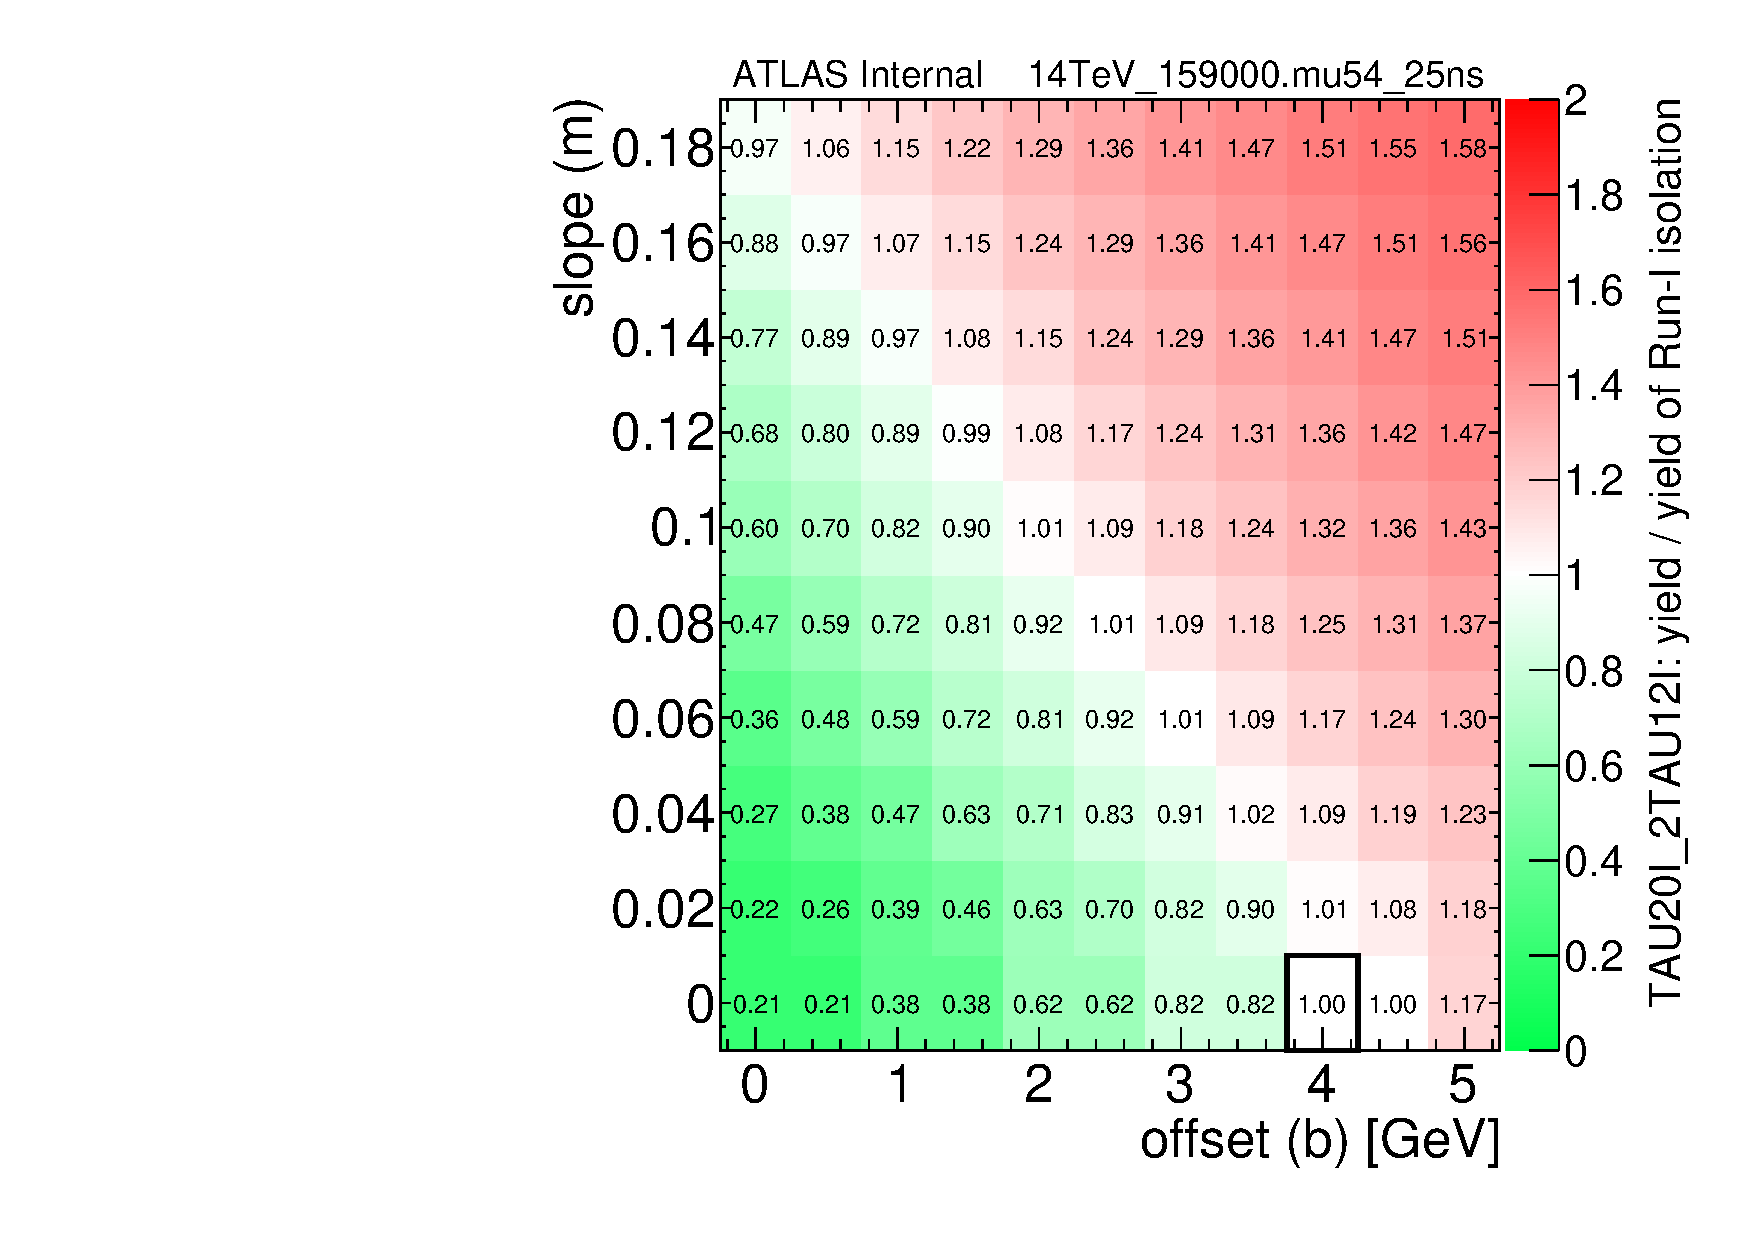
\includegraphics[width=0.48\textwidth]{figures/trigger/iso_background_noTAU60}
  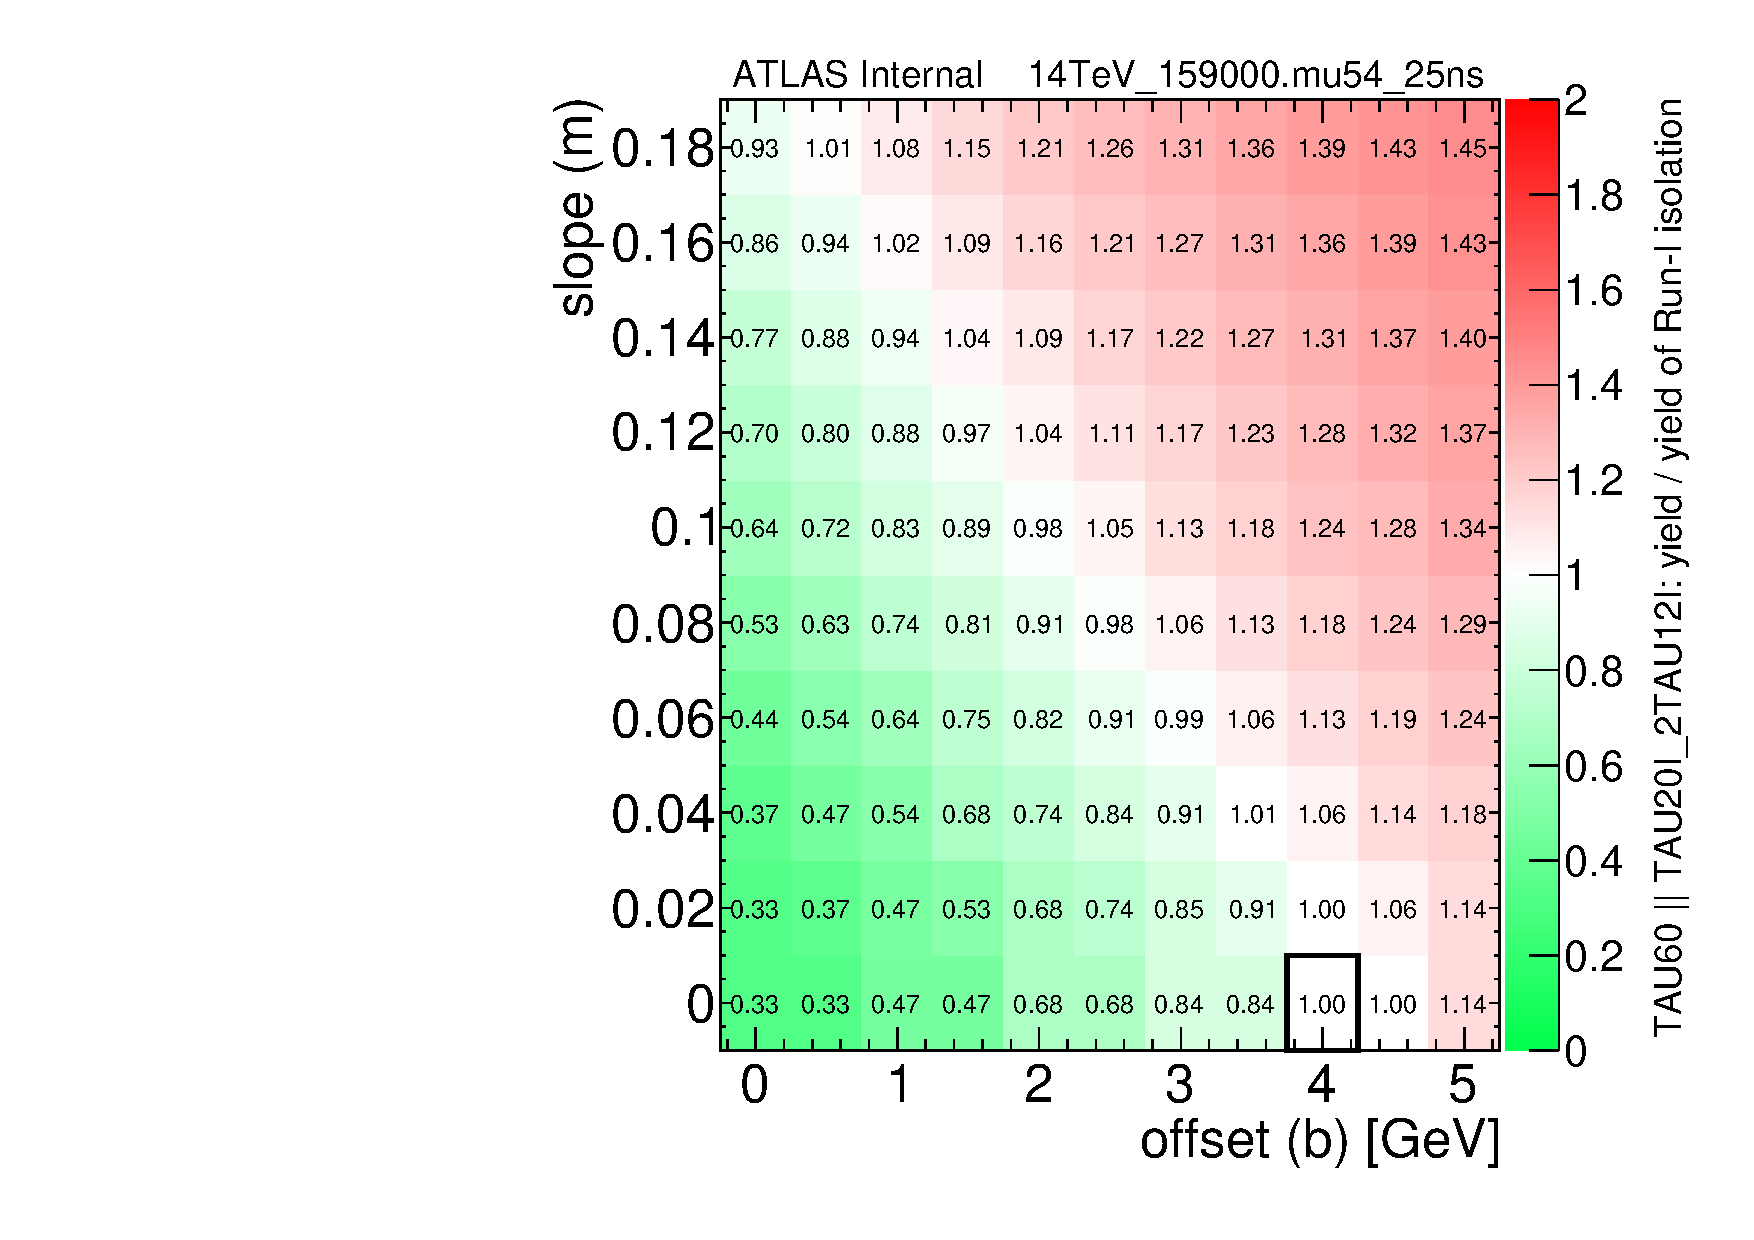
\includegraphics[width=0.48\textwidth]{figures/trigger/iso_background_yesTAU60}
  \caption{L1 rate for the di-$\tauh$ trigger in 14 TeV minimum bias MC for various $\pt^\text{L1}$-dependent isolation definitions relative to the 2012 definition: $\pt^\text{L1,iso} \leq 4$ GeV. Many options give the same rate (white color). The rate is calculated irrespective of the lowest unprescaled single $\tauh$ trigger (left) and with a logical \texttt{OR} of it (right).}
  \label{fig:prospects-trigger-isolation-rate}
\end{figure}

\begin{figure}[!htpb]
  \centering
  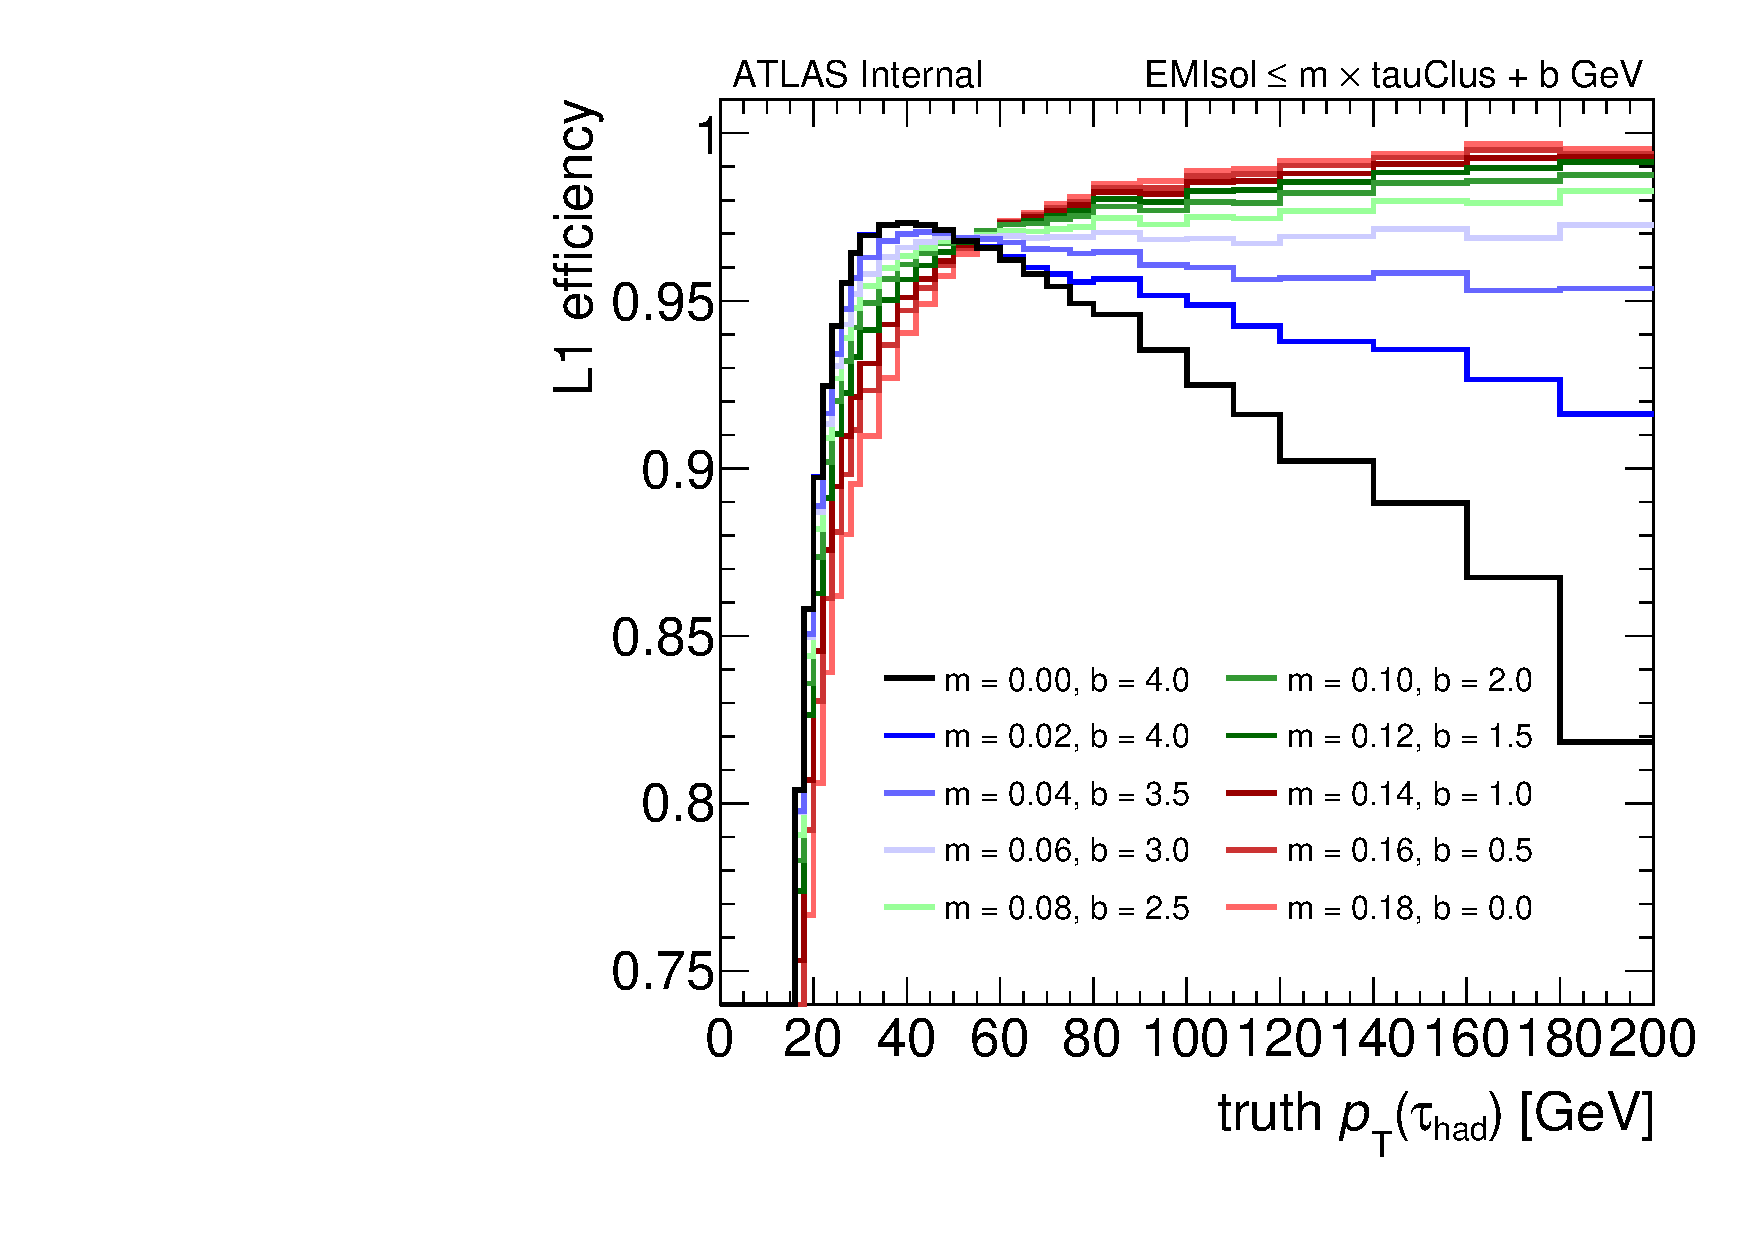
\includegraphics[width=0.48\textwidth]{figures/trigger/iso_turnonL1_noTAU60}
  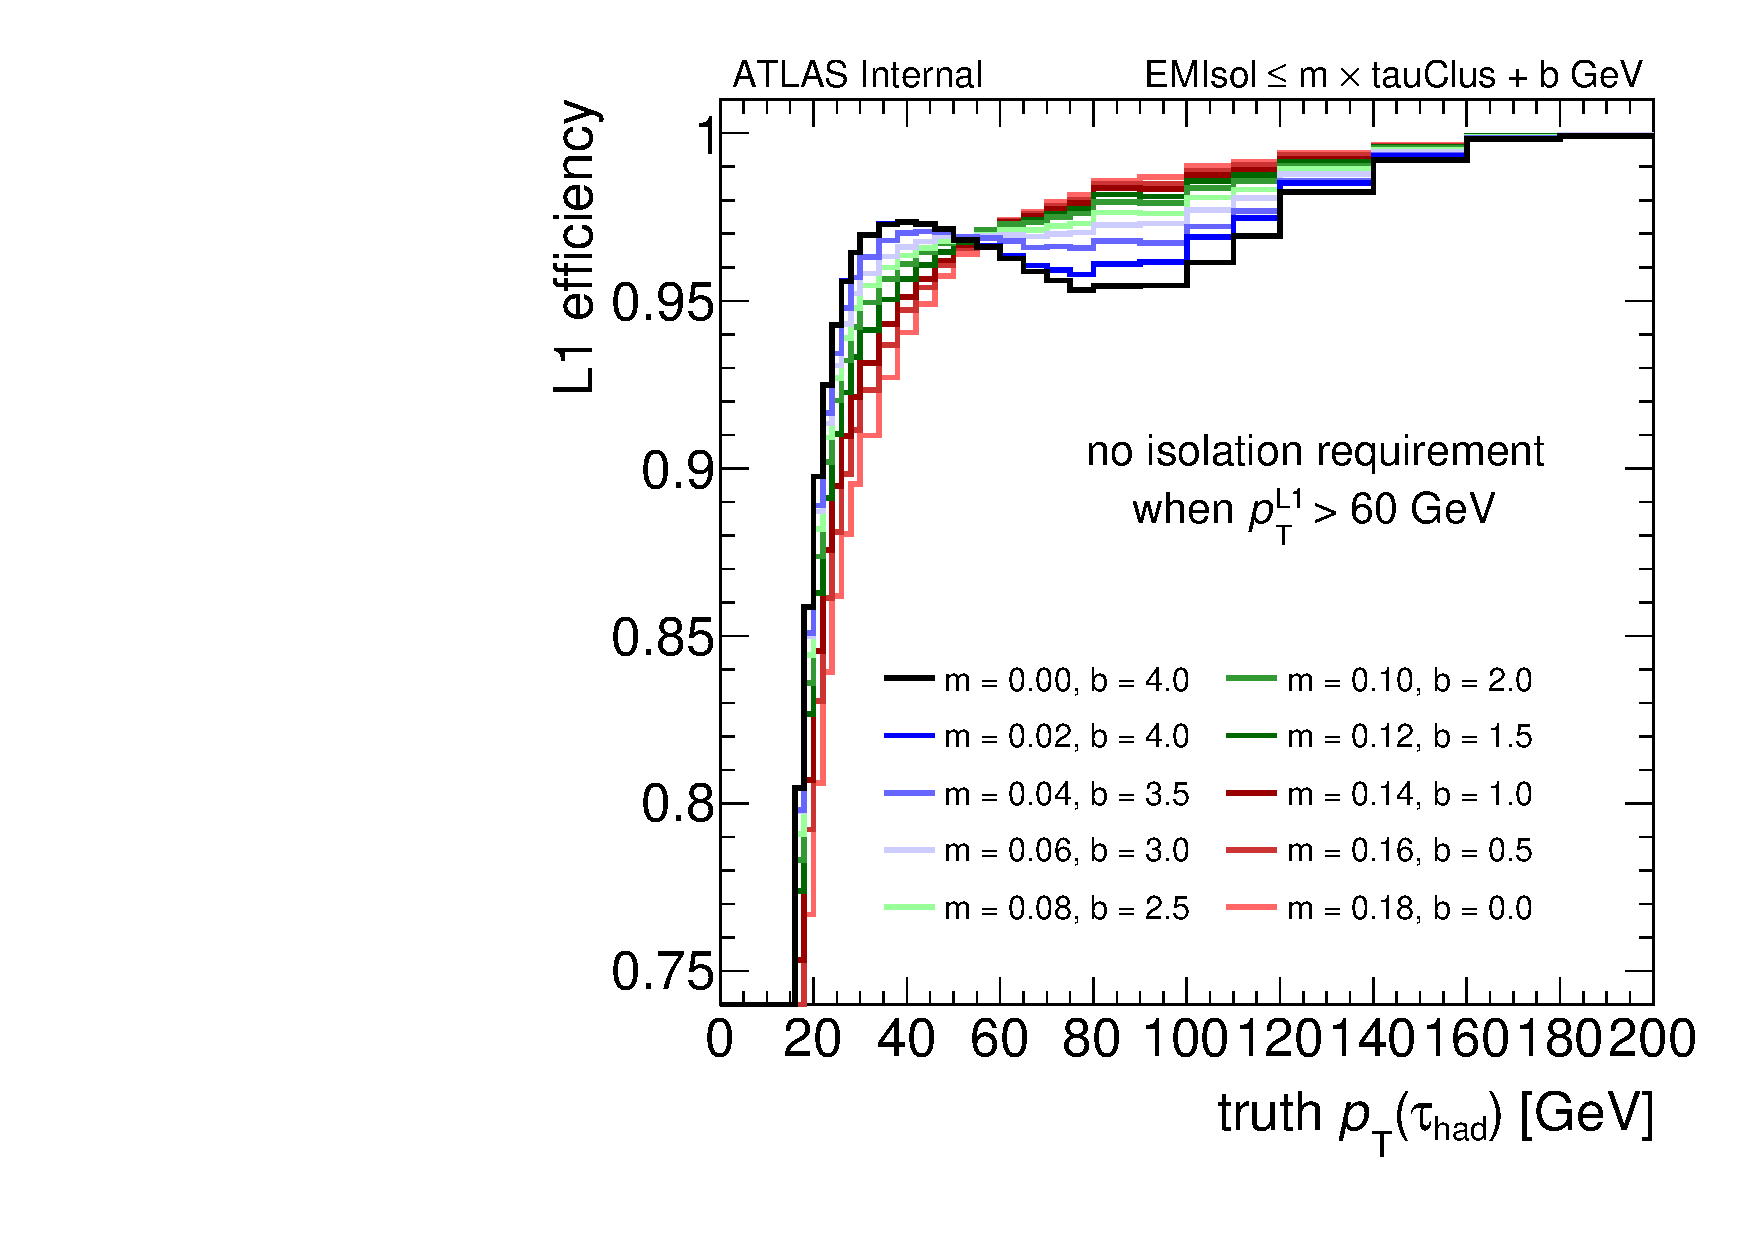
\includegraphics[width=0.48\textwidth]{figures/trigger/iso_turnonL1_yesTAU60}
  \caption{Efficiency for firing the L1 $\tauh$ trigger for various $\pt^\text{L1}$-dependent isolation definitions which have similar rates, as derived from \cref{fig:prospects-trigger-isolation-rate}. The 2012 definition is the black line. The efficiency is calculated irrespective of the lowest unprescaled single $\tauh$ trigger (left) and with a logical \texttt{OR} of it (right).}
  \label{fig:prospects-trigger-isolation-turnon}
\end{figure}

\subsection{Conclusions and contingencies}

Despite significantly harsher data-taking conditions in 2015, triggers for the $\Htautauhh$ and $\Htautaulh$ analyses can be adapted to retain physics output with manageable rates and without major loss of generality. The most important adaptations for both channels are requiring an additional high-$\pt$ jet and requiring low $\Delta R(\tautau)$. The L1 $\tauh$ menu is shown in \cref{tab:prospects-taumenu}.

\begin{table}[!htpb]
  \centering
  \renewcommand{\arraystretch}{1.4}
  \caption{The $\tauh$ L1 menu. A baseline L1 menu is used for calculating the unique rate.}
  \begin{tabular}{c|c|c|c}
  signature      & target        & L1 item                           & unique rate [kHz] \\
  \hline\hline
  single $\tauh$ & exotics, SUSY & \texttt{TAU60V}                   & 1.6 \\
  di-$\tauh$     & Higgs, di-$H$ & \texttt{TAU12I\_TAU20I\_J25-DR28} & 3.7 \\
  \hline
  $e   + \tauh$  & Higgs         & \texttt{EM15HI\_TAU12I\_J25-DR28} & 1.2 \\
  $e   + \tauh$  & exotics, SUSY & \texttt{EM15HI\_TAU40}            & 0.2 \\
  $\mu + \tauh$  & Higgs         & \texttt{TAU12I\_MU10\_J25-DR28}   & 0.5 \\
  $\mu + \tauh$  & exotics, SUSY & \texttt{TAU20\_MU10}              & 0.5 \\
  \hline
  $\tauh + \MET$ & SUSY          & \texttt{TAU20\_XE45\_J20}         & 0.5 \\
  $\tauh + \MET$ & SUSY          & \texttt{TAU12I\_TAU20I\_XE35}     & 2.1 \\
  $\tauh + \MET$ & SUSY          & \texttt{EM15HI\_TAU12I\_XE35}     & 0.2 \\
  $\tauh + \MET$ & SUSY          & \texttt{TAU12I\_MU10\_XE35}       & 0.0 \\
  \hline\hline
\end{tabular}


  \label{tab:prospects-taumenu}
\end{table}

Contingency plans are considered due to the uncertainty of the rate prediction and the uncertainty of the LHC data-taking conditions.

\begin{table}[!htpb]
  \centering
  \renewcommand{\arraystretch}{1.4}
  \caption{Contingency options for the $\Htautau$ section of the $\tauh$ L1 menu. The change in unique rate is with respect to the baseline menu. A baseline L1 menu is used for calculating the unique rate.}
  \begin{tabular}{c|c|c|c}
  scenario       & item change   & motivation                        & $\Delta$(rate) [kHz] \\
  \hline\hline
  add rate, 3rd option & \texttt{TAU20I} $\rightarrow$ \texttt{TAU15I}                    & slow $\tauh$ turn-on                        & +3.2 \\
  add rate, 2nd option & \texttt{$\Delta R(\tautau) < 2.8 \rightarrow 3.0$}               & $\Delta R(\tautau)$ inefficiency for di-$H$ & +2.6 \\
  add rate, 1st option & \texttt{J25} $\rightarrow$ \texttt{J20}                          & slow jet turn-on                            & +0.4 \\
  baseline             & --                                                               & --                                          & --   \\
  cut rate, 1st option & \texttt{TAU12I} $\rightarrow$ \texttt{TAU20I} ($\ell\!+\!\tauh$) & small gain with $\ell+\tauh$ triggers       & -1.7 \\
  cut rate, 2nd option & \texttt{J25} $\rightarrow$ \texttt{J30}                          & jet threshold is least painful              & -2.2 \\
  cut rate, 3rd option & \texttt{TAU20I} $\rightarrow$ \texttt{TAU25I}                    & $\tauh$ threshold is second least           & -3.8 \\
  \hline\hline
\end{tabular}

  \label{tab:prospects-contingencies}
\end{table}

\clearpage

\section{HL-LHC}
\label{sec:prospects-hllhc}

This section documents projections of the Standard Model $\Htautau$ analysis for the ECFA High Luminosity LHC Experiments Workshop 2014~\cite{ATL-PHYS-PUB-2014-018}. The projection considers High Luminosity LHC (HL-LHC) running conditions with 14 TeV $pp$ collisions, 3000 $\ifb$ delivered integrated luminosity, and an average number of overlapping $pp$ collisions per bunch-crossing (pile-up) $\pileup = 140$. Only the VBF $\taul\tauh$ ($\ell = e,\mu$) analysis category is considered.

This projection is built from the existing Run-I analysis~\cite{HIGG-2013-32} by using the same data samples, Monte Carlo samples, data-driven background estimates, and multivariate analysis (MVA) techniques. It is projected to HL-LHC conditions by adding emulation of the harsher pile-up conditions and scaling the predictions by the ratios of cross-sections and integrated luminosity for HL-LHC versus 2012 conditions. The harsher pile-up conditions impacts jets and $\MET$ significantly.

The analysis also considers possible extensions of the tracking volume to investigate the impact of tracking-based rejection of pile-up jets. 

\subsection{Selection}

The selection of a VBF-like sample for the $\taul\tauh$ final state discussed in this note relies on the identification of one lepton (electron or muon), one hadronic tau and at least two jets. Muons are selected if they have transverse momentum higher than $26 \GeV$ and are in the region $|\eta|<2.4$. Quality criteria on the inner detector track associated to the muon are also applied. Electron candidates are formed from a cluster in the electromagnetic calorimeters (transition regions, $1.37<|\eta|<1.52$, are excluded) that is matched with a track reconstructed within the inner detector, $|\eta|<2.47$. Electrons with a transverse momentum higher than $26~\GeV$ are selected and a \texttt{tightPP} working point is used. For both muons and electrons, calorimeter and track-based isolation criteria with similar combined selection efficiency as the LHC Run-I analysis are assumed.

Jets are reconstructed using the anti-$k_t$ algorithm~\cite{Antikt1} with a radius parameter $R=0.4$, taking topological clusters in the calorimeters as inputs. Only jets with $|\eta|<4.5$ are selected in this analysis. The general $\pt$ threshold for jets is 30 GeV, and specific selection of the VBF analysis is mentioned later. Track-based pile-up suppression with jet-vertex fraction (JVF)~\cite{ATLAS-CONF-2014-018} is applied in the range of the tracking volume (jet $|\eta| < 2.4$). In the range $\left|\eta\right|<2.5$, $b$-tagged jets are identified using the MV1 tagging algorithm based on the impact parameter information and on the reconstruction of the displaced vertices of the hadron decays inside the jets~\cite{ATLAS-CONF-2014-046}. 

Tau candidates are seeded by anti-$k_t$~\cite{Antikt1}, $R=0.4$ jets with $\pt > 20$ GeV whose calorimeter cluster and leading track must satisfy $|\eta| < 2.47$. The Boosted Decision Tree (BDT) tau identification method~\cite{PERF-2013-06} is used, requiring that the tau candidate passes the \texttt{medium} tightness, corresponding to to approximately 55-60\% efficiency A dedicated selection to reject fake tau candidates from electrons and muons is applied.

When different objects selected according to the above criteria overlap with each other geometrically (within $\Delta R < 0.2$), only one of them is considered for further analysis. The overlap is resolved by selecting muon, electron, $\tauh$ and jet candidates in this order of priority.

The signal events are characterized by true $\MET$ due to the presence of the neutrinos from the tau decays. In this analysis, the $\MET$ reconstruction uses reconstructed high-$\pt$ physics objects (electrons, photons, $\tauh$, jets and muons) and a measurement of the soft term, which includes contributions from the underlying event, multi-parton interactions, and physics objects below analysis threshold.

Unless otherwise noted, the topological selection criteria are identical to the Run-I analysis. One lepton and one hadronically decaying tau are required, and there must be at least two jets with a significant separation in $\eta$ as expected for VBF production. Some additional topological cuts are applied to suppress backgrounds while retaining most of the signal. The VBF category is intentionally defined loosely since the discrimination of signal from background is meant to be handled by the BDTs. The event selection is summarized in \cref{tab:prospects-HLLHC-selection}.

\begin{table}[!htpb]
  \centering
  \renewcommand{\arraystretch}{1.4}
  \caption{Event selection and categorization criteria. The $\mT$ requirement is relaxed to avoid signal loss due to the degradation of the $\MET$ resolution at high $\pileup$.}
  \begin{tabular}{c|c}
  Type                                      & Selection                                                      \\
  \hline\hline
  \multirow{4}{*}{$\tautaulh$ preselection} & exactly one identified and isolated lepton ($e,\mu$)           \\
                                            & exactly one identified tau                                     \\
                                            & opposite sign lepton and tau                                   \\
                                            & no additional leptons passing loosened identification criteria \\
                                            & no jets passing the $b$-tagging criteria                       \\
                                            & $\mT < 100$ GeV                                                \\
  \hline
  \multirow{4}{*}{VBF categorization}       & leading jet with $\pt > 50$ GeV                                \\
                                            & any additional jet with $\pt > 30$ GeV                         \\
                                            & $|\Delta\eta(\text{lead jet}, \text{sub-lead jet})| > 3.0$     \\
                                            & $\mvis > 40 \GeV$ \\
\end{tabular}


  \label{tab:prospects-HLLHC-selection}
\end{table}

\subsection{Emulation of High-Luminosity LHC conditions}

The method of pile-up emulation follows the same procedure used by the $\HWW$ projection for ECFA 2013~\cite{ATL-PHYS-PUB-2013-014}. The approach is to port the existing Run-I analysis to HL-LHC conditions by overlaying pile-up jets on the 8 TeV samples, degrading the hard-scatter (HS) jet and $\MET$ resolution, and propagating the impact of this to the analysis.

\subsubsection{Performance assumptions}

The Run-I triggering thresholds and efficiency are assumed. The ATLAS trigger has many upgrades planned to mitigate the impact of higher instantaneous luminosity, including the New Small Wheel, hardware trackers, and finer L1 EM-calorimeter granularity. Improvements to the L1 granularity will especially improve triggers with electrons and taus, since shower shape variables can be built to discriminate against QCD jets better than existing isolation variables. It is then deemed unnecessary to consider scenarios of significant trigger efficiency loss in detail.

It is also assumed that the lepton and tau reconstruction and identification efficiencies are equivalent to that observed in the 2012 data. This is chosen because the detector upgrades for the HL-LHC aim for achieving a performance similar to Run-I despite the harsher pile-up conditions. Hard-scatter jets from the 8 TeV samples are smeared to emulate the reconstructed jet resolution at HL-LHC conditions~\cite{ATL-PHYS-PUB-2013-004}. The jet smearing is propagated to the $\MET$ calculation. The soft-term resolution of the $\MET$ is smeared: 33 MeV per unit of $\pileup$, which is derived from high pile-up $Z/\gamma^\ast$ simulation.

\subsubsection{Pileup emulation}

Pileup jets are inserted into the event according to rates recommended by the ATLAS projections~\cite{ATL-PHYS-PUB-2013-004}. For $\pileup=140$ and jet $\pt \ge 30 \GeV$, the rate is 2.4 additional pile-up jets per event. The kinematics of the inserted pile-up jets are derived from high pile-up $Z/\gamma^\ast$ simulation. Templates are built for $\pt$ and $\eta$ and are then randomly sampled for each inserted pileup jet. 

The hard-scattering jets are assumed to have a reconstruction efficiency of the track-confirmation algorithm recommended by the existing ATLAS projections. The pile-up jets are assumed to have the pile-up suppression efficiency of the 2012 JVF algorithm, which is 98\% within the tracking volume~\cite{ATLAS-CONF-2014-018}. No degradation of pile-up jet suppression is assumed because techniques already exist which out-perform the JVF tagger. The pile-up suppression is assumed to not depend on $\pt$ and $\eta$ other than at the boundary of the tracker. The insertion of pileup jets is then propagated to the $\MET$ calculation.

A new tracker in the forward region $|\eta| > 2.5$ is being considered for Phase-II ATLAS upgrades. To emulate the impact of pile-up jet suppression with a forward tracker, the analysis is re-run with forward pile-up jet rejection imposed by hand. Since the scope of the forward tracker is uncertain, a range of coverage and performance is considered: coverage of $|\eta| < $ 3.0, 3.5, and 4.0 and pile-up jet suppression of 50\%, 75\%, and 90\% with negligible signal (hard-scattering jets) efficiency loss is evaluated. For comparison, a pile-up jet suppression of 90\% with negligible signal efficiency loss is comparable to the performance of the JVF tagger within the existing tracker~\cite{ATLAS-CONF-2014-018}.

The method of randomly inserting pile-up jets into existing events does not consider correlations between pile-up jets. This could be problematic because the $\pt$ imbalance of the event could be overstated, which would propagate to unphysical biases of quantities which are sensitive to balance like $\MET$. The impact of this has been assessed by overlaying entire truth pile-up events onto the existing hard scatter events. The results are comparable.

\subsubsection{Impact on observables}

The VBF $\Htautau$ analysis relies on two jets with large $\Delta\eta$ to describe the VBF topology and on $\MET$ to describe di-$\tau$ decays. The presence of forward pile-up jets can then be expected to degrade the sensitivity of the analysis because they will cause migration of background events into the VBF category, and because they will bias the $\MET$ calculation.

The contamination of pile-up jets in the VBF category for the total background is significant. Most events (72\%) have a sub-lead pile-up jet, and nearly half (42\%) have a lead pile-up jet. These pile-up jets are especially problematic because they are typically forward, thus any event with pile-up lead and sub-lead jets in opposite hemispheres will have $|\eta_{j1} - \eta_{j2}| > 4.8$.

Degradation of the $\MET$ and MMC $m(\tau\tau)$ under the high-luminosity conditions is shown in \cref{fig:prospects-hllhc-degradation} for simulated VBF $\Htautau$. Both observables are degraded by jet and $\MET$ smearing and by the presence of forward pile-up jets biasing the $\MET$ calculation.

\begin{figure}[!htpb]
  \centering
  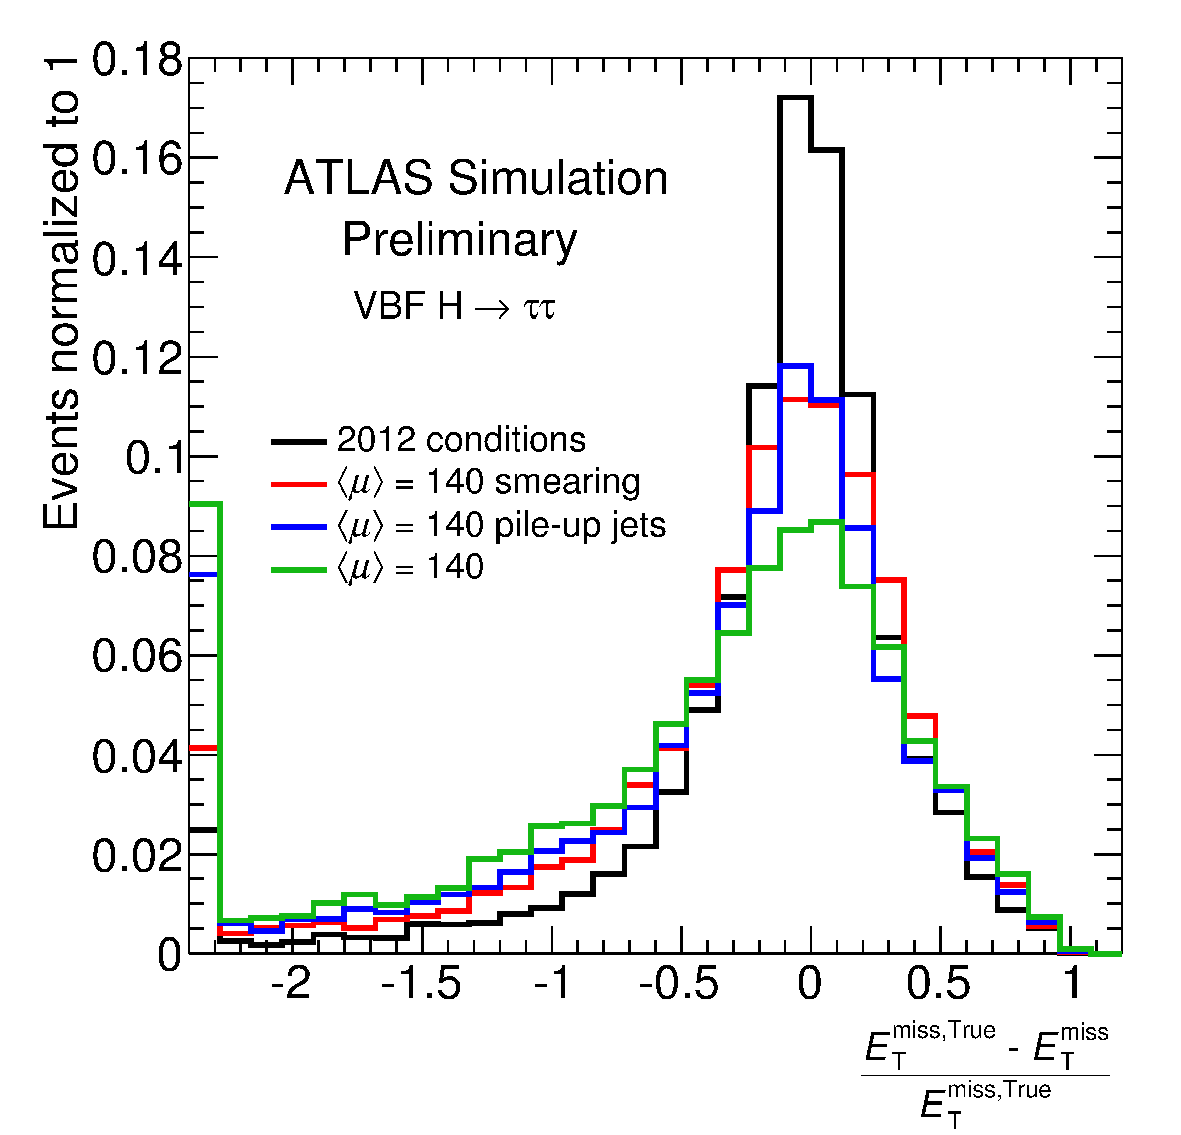
\includegraphics[width=0.48\textwidth]{figures/ATL-PHYS-PUB-2014-018/fig_01a}
  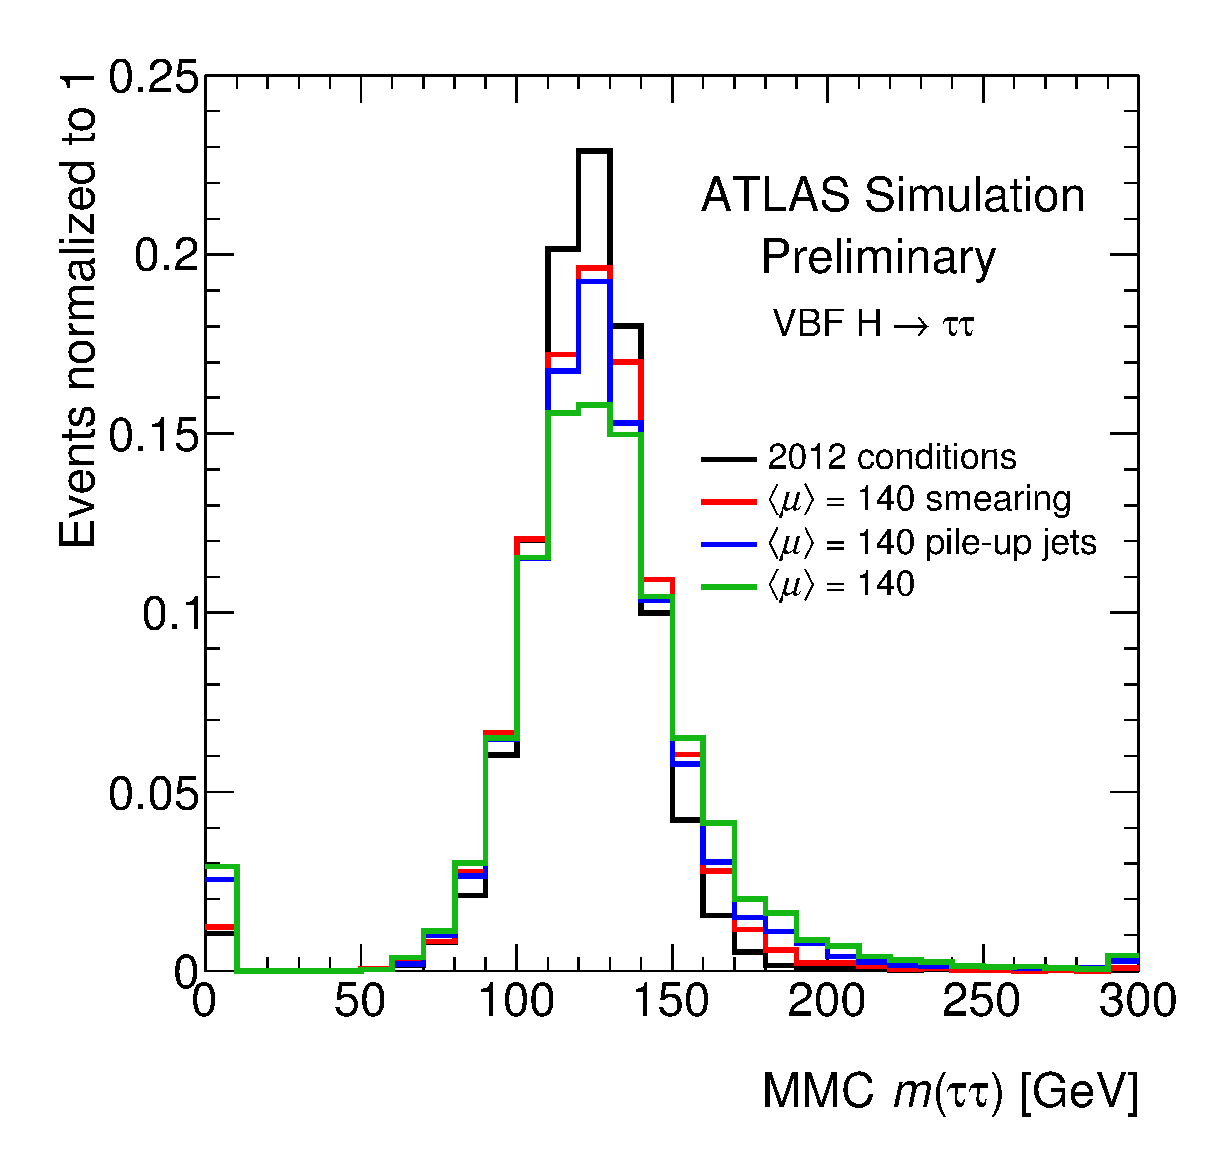
\includegraphics[width=0.48\textwidth]{figures/ATL-PHYS-PUB-2014-018/fig_01b}
  \caption{Degradation of $\MET$-related observables at HL-LHC conditions for VBF $\Htautaulh$: the $\MET$ resolution (left) and reconstructed $\mMMC$ (right)~\cite{ATL-PHYS-PUB-2014-018}. The underflow of the $\mMMC$ shows the fraction of events which fail the mass reconstruction.}
  \label{fig:prospects-hllhc-degradation}
\end{figure}

\subsection{Analysis}

\subsubsection{Boosted decision tree training}

A multi-variate analysis approach is used by training BDTs to discriminate signal from background. It is trained using all backgrounds scaled to their respective cross-sections against the total (ggF + VBF) signal shapes. The same training parameters and input variables as the Run-I analysis are used, and the input variables are listed in \cref{tab:prospects-hllhc-inputs}.

\begin{table}[!htpb]
  \centering
  \renewcommand{\arraystretch}{1.4}
  \caption{Discriminating variables used for the BDT training.}
  \begin{tabular}{c|c}
  Variable                        & Definition                                              \\
  \hline
  $\Delta R(\tauh, \ell)$         & Separation of the lepton and $\tauh$                    \\
  $\mT$                           & Transverse mass of the lepton and $\MET$                \\
  $\MET\phi$-centrality           & Centrality of the $\MET$ between the lepton and $\tauh$ \\
  MMC $\mtautau$                  & $\tau\tau$ mass estimator                               \\
  $m_{j1,j2}$                     & Invariant mass of the 2 leading jets                    \\
  $\eta_{j1}\times\eta_{j2}$      & Product of the $\eta$s of the two leading jets          \\
  $|\eta_{j1} - \eta_{j2}|$       & Absolute difference $\eta$s of the two leading jets     \\
  $\ell$ $\eta$-centrality        & Centrality of the lepton between the two leading jets   \\
  $p_{\text{T}}^{\mathrm{Total}}$ & $|\vec{p}_{\mathrm{T}}^{\ell} + \vec{p}_{\mathrm{T}}^{\tau_h} + \vec{p}_{\mathrm{T}}^{\mathrm{j1}} + \vec{p}_{\mathrm{T}}^{\mathrm{j2}} + \vec{E}_{\mathrm{T}}^{\mathrm{miss}}|$ \\   
\end{tabular}


  \label{tab:prospects-hllhc-inputs}
\end{table}

BDTs are trained for a variety of forward tracker coverages ($|\eta| < 3$, $|\eta| < 3.5$ and $|\eta| < 4$) and pile-up rejection values (50\%, 75\% and 90\%). \cref{fig:prospects-hllhc-rocs} shows the efficiency for rejecting the background versus the efficiency for selecting the signal for the scenario of 90\% forward pile-up rejection. For a given signal efficiency, the background rejection improves with larger coverage.

\begin{figure}[!htpb]
  \centering
  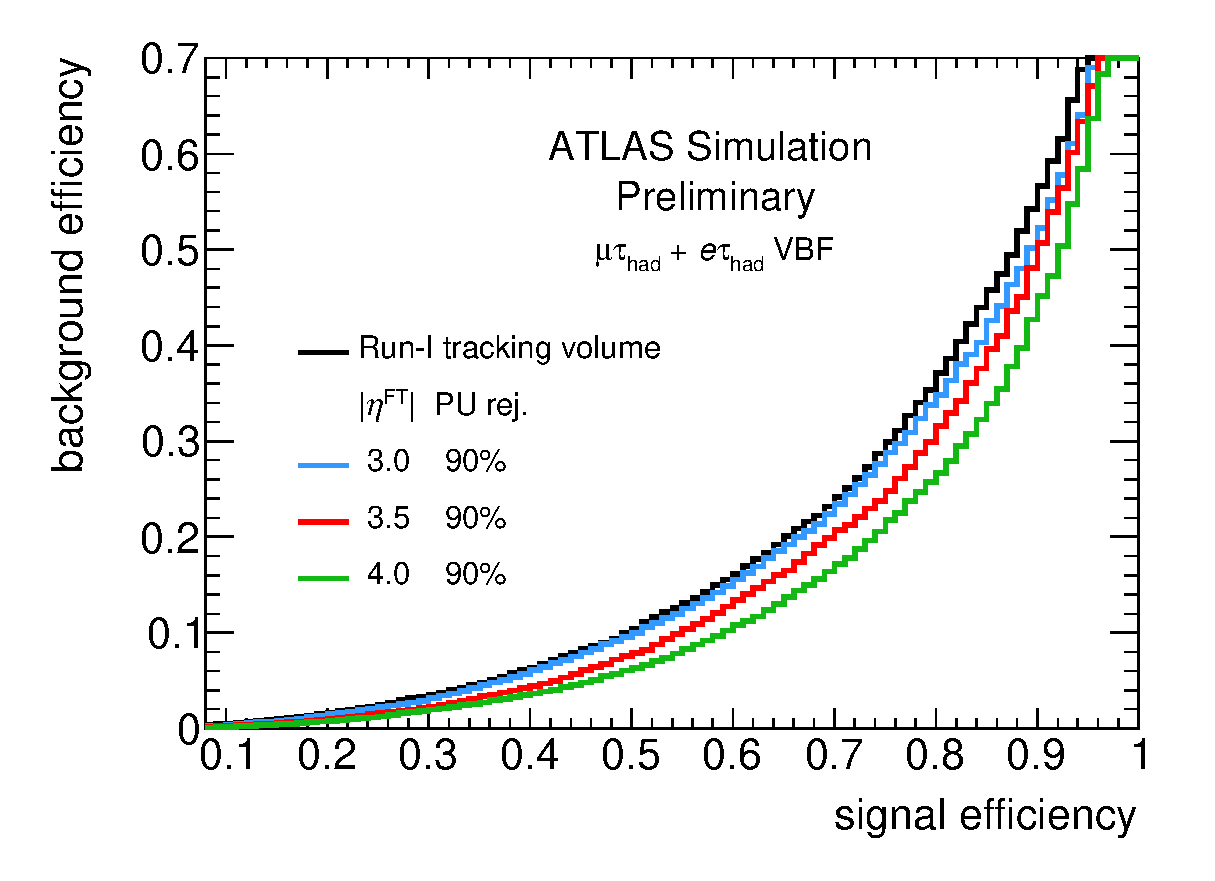
\includegraphics[width=0.48\textwidth]{figures/ATL-PHYS-PUB-2014-018/fig_02a}
  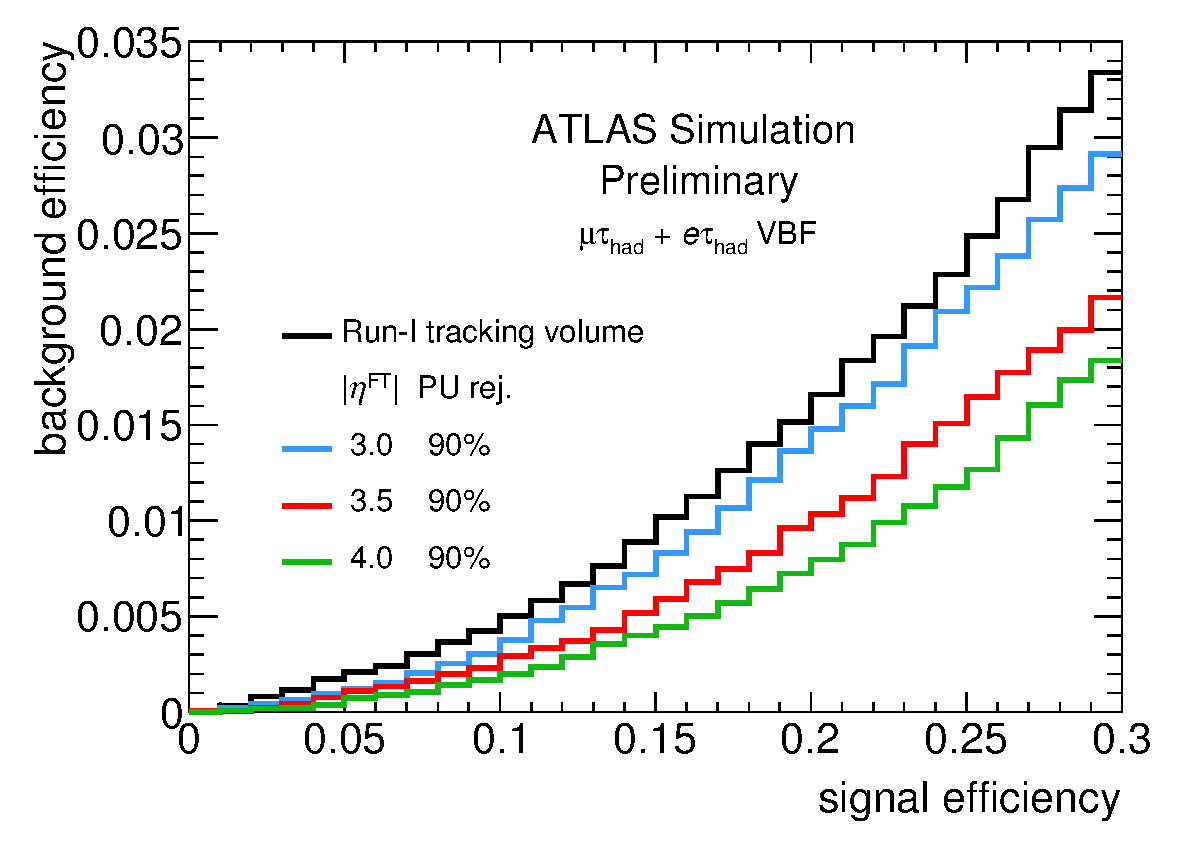
\includegraphics[width=0.48\textwidth]{figures/ATL-PHYS-PUB-2014-018/fig_02b}
  \caption{Signal efficiency versus background efficiency for scenarios of generic forward tracker coverage and rejection power (left) and zoomed in to lower signal efficiency (right)~\cite{ATL-PHYS-PUB-2014-018}. A BDT is trained in the VBF category for each scenario.}
  \label{fig:prospects-hllhc-rocs}
\end{figure}

\subsubsection{Kinematic distributions}

Predicted signal and background BDT input distributions as well as basic object kinematics are shown in Figures \cref{fig:prospects-hllhc-jets}, \cref{fig:prospects-hllhc-taus} and \cref{fig:prospects-hllhc-other}. Signal and background are predicted with the same methods as the Run-I analysis~\cite{HIGG-2013-32}, including the data-driven prediction of the dominant $\Ztautau$ and fake backgrounds. The resulting BDT score is presented in Figure \cref{fig:prospects-hllhc-bdts}.

\begin{figure}[!htpb]
  \centering
  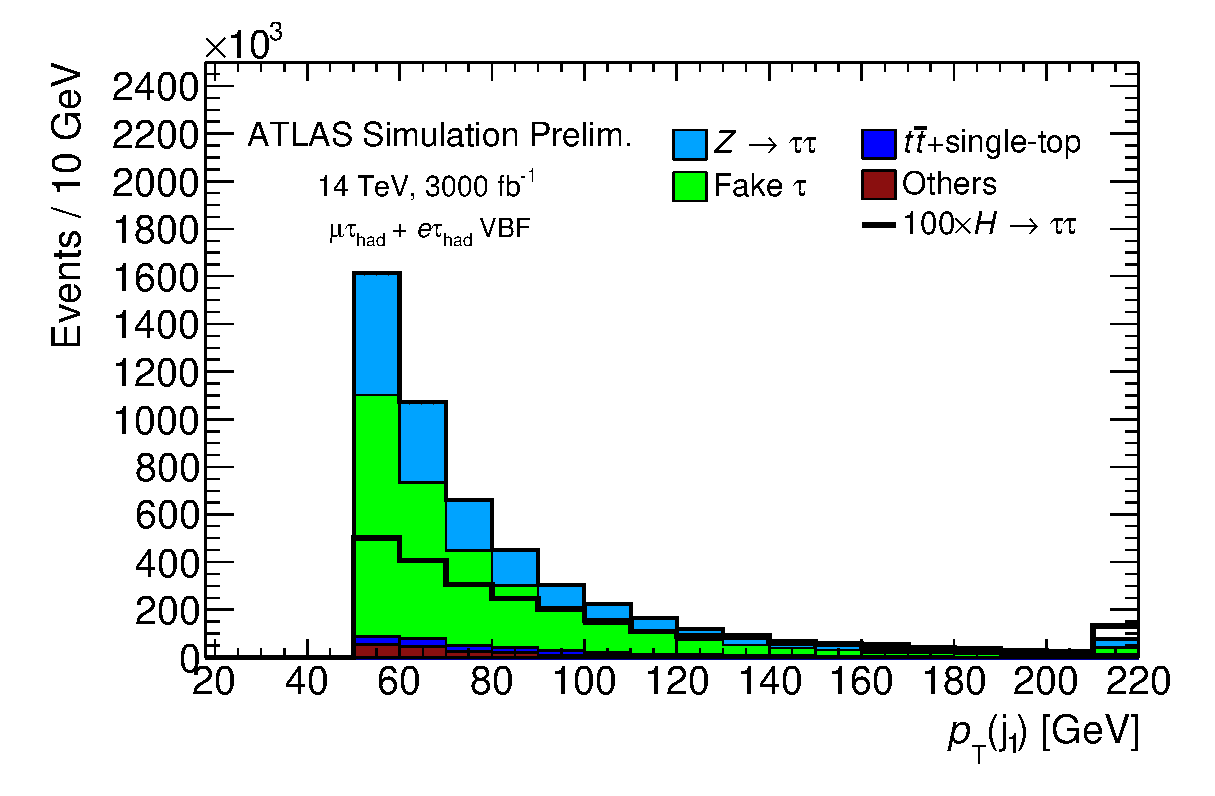
\includegraphics[width=0.48\textwidth]{figures/ATL-PHYS-PUB-2014-018/fig_03a}
  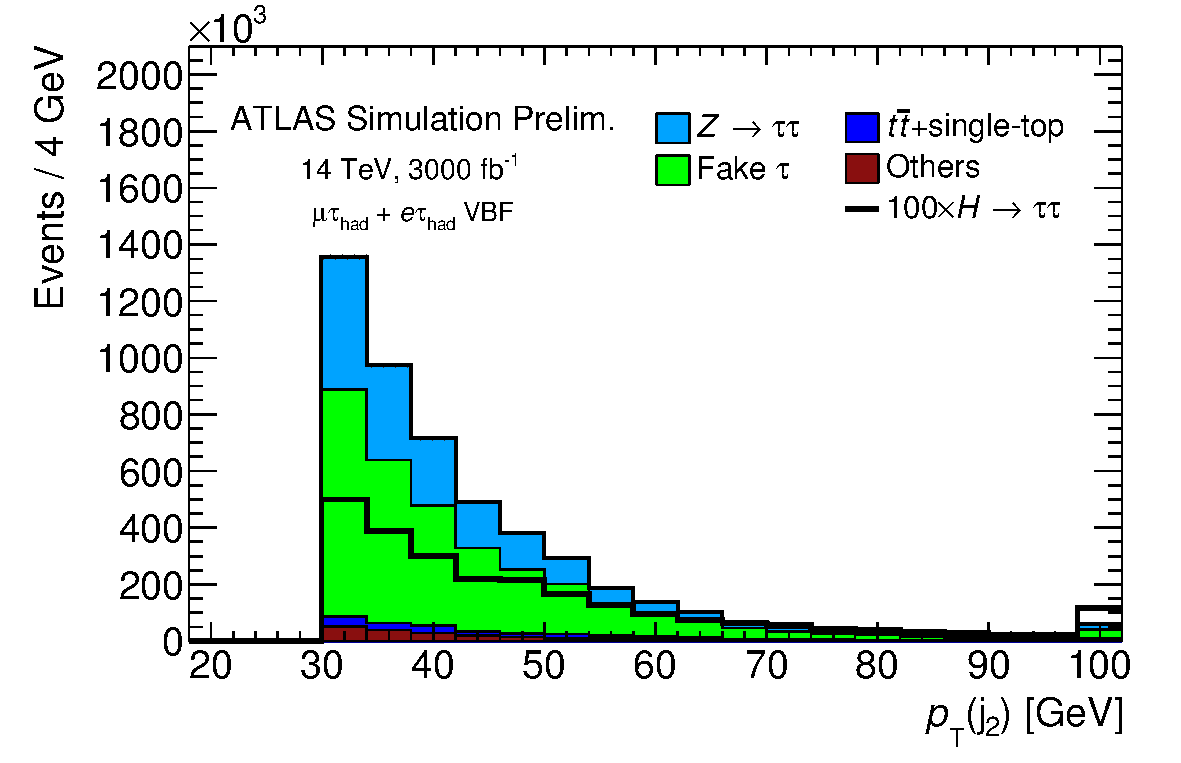
\includegraphics[width=0.48\textwidth]{figures/ATL-PHYS-PUB-2014-018/fig_03b}
  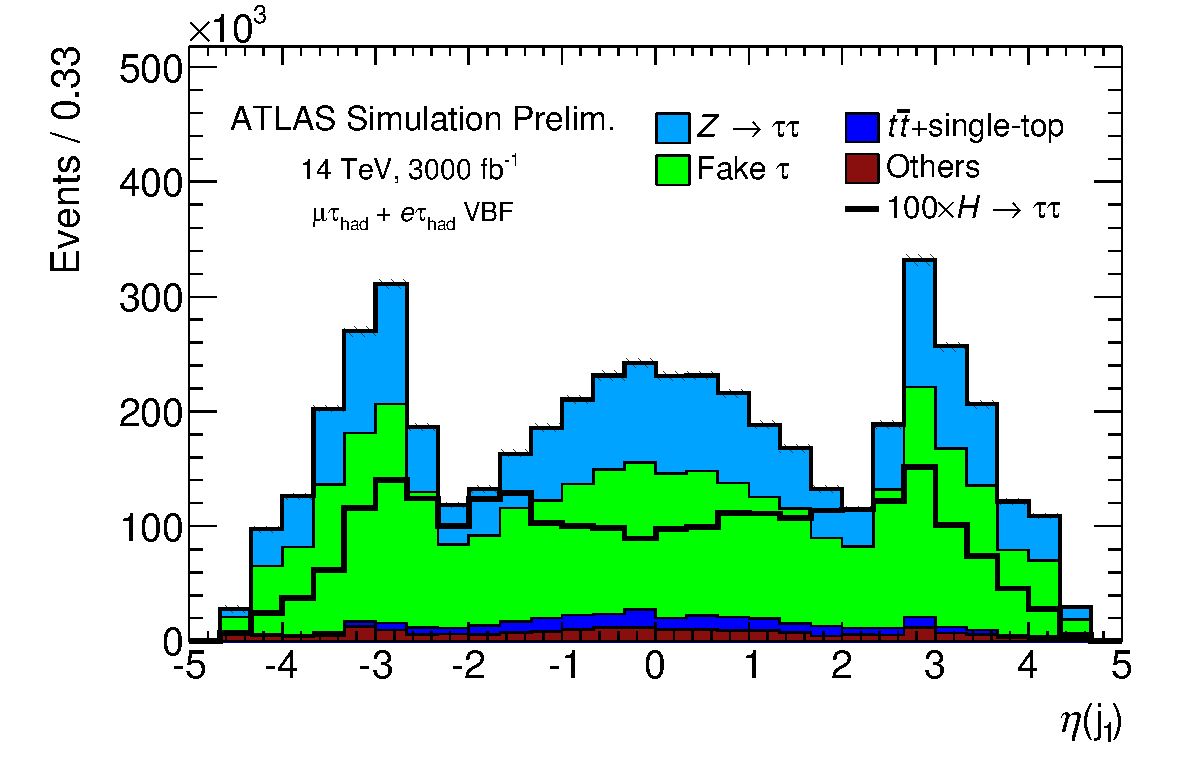
\includegraphics[width=0.48\textwidth]{figures/ATL-PHYS-PUB-2014-018/fig_03c}
  \includegraphics[width=0.48\textwidth]{figures/ATL-PHYS-PUB-2014-018/fig_03d}
  \includegraphics[width=0.48\textwidth]{figures/ATL-PHYS-PUB-2014-018/fig_03e}
  \includegraphics[width=0.48\textwidth]{figures/ATL-PHYS-PUB-2014-018/fig_03f}
  \includegraphics[width=0.48\textwidth]{figures/ATL-PHYS-PUB-2014-018/fig_03g}
  \includegraphics[width=0.48\textwidth]{figures/ATL-PHYS-PUB-2014-018/fig_03h}
  \caption{Signal and background HL-LHC predictions of (a) leading jet $\pt$, (b) sub-leading jet $\pt$, (c) leading jet $\eta$, (d) sub-leading jet $\eta$, (e) $\Delta\eta_{jj}$, (f) $m_{jj}$, (g) $\eta_{lead jet}\times \eta_{sub-lead jet}$ and (h) $\MET$~\cite{ATL-PHYS-PUB-2014-018}. The last bin contains the overflow events.}
  \label{fig:prospects-hllhc-jets}
\end{figure}

\begin{figure}[!htpb]
  \centering
  \includegraphics[width=0.48\textwidth]{figures/ATL-PHYS-PUB-2014-018/fig_04a}
  \includegraphics[width=0.48\textwidth]{figures/ATL-PHYS-PUB-2014-018/fig_04b}
  \includegraphics[width=0.48\textwidth]{figures/ATL-PHYS-PUB-2014-018/fig_04c}
  \includegraphics[width=0.48\textwidth]{figures/ATL-PHYS-PUB-2014-018/fig_04d}
  \includegraphics[width=0.48\textwidth]{figures/ATL-PHYS-PUB-2014-018/fig_04e}
  \includegraphics[width=0.48\textwidth]{figures/ATL-PHYS-PUB-2014-018/fig_04f}
  \includegraphics[width=0.48\textwidth]{figures/ATL-PHYS-PUB-2014-018/fig_04g}
  \includegraphics[width=0.48\textwidth]{figures/ATL-PHYS-PUB-2014-018/fig_04h}
  \caption{Signal and background HL-LHC predictions of (a) $\pt(\tauh)$, (b) $\pt(\text{lepton})$, (c) $\eta(\tauh)$, (d) $\eta(\text{lepton})$, (e) $\Delta R(\tauh, \text{lepton})$, (f) MMC (g) $\mvis$ and (h) $\mT$~\cite{ATL-PHYS-PUB-2014-018}. The last bin contains the overflow events.}
  \label{fig:prospects-hllhc-taus}
\end{figure}

\begin{figure}[!htpb]
  \centering
  \includegraphics[width=0.32\textwidth]{figures/ATL-PHYS-PUB-2014-018/fig_05a}
  \includegraphics[width=0.32\textwidth]{figures/ATL-PHYS-PUB-2014-018/fig_05b}
  \includegraphics[width=0.32\textwidth]{figures/ATL-PHYS-PUB-2014-018/fig_05c}
  \caption{Signal and background HL-LHC predictions of (a) $\MET \phi$-centrality, (b) $\text{lepton}$ $\eta$-centrality and (c) $\pt^\text{Total}$~\cite{ATL-PHYS-PUB-2014-018}. The last bin contains the overflow events.}
  \label{fig:prospects-hllhc-other}
\end{figure}

\begin{figure}[!htpb]
  \centering
  \includegraphics[width=0.48\textwidth]{figures/ATL-PHYS-PUB-2014-018/fig_06a}
  \includegraphics[width=0.48\textwidth]{figures/ATL-PHYS-PUB-2014-018/fig_06b}
  \caption{Signal and background HL-LHC predictions of the BDT spectrum in the (a) full range and (b) highest bins range~\cite{ATL-PHYS-PUB-2014-018}. Signal and background are overlaid in (a) and stacked in (b).}
  \label{fig:prospects-hllhc-bdts}
\end{figure}

\subsection{Results}

Yields for signal and background in the high BDT score bins are shown in \cref{tab:prospects-hllhc-yields}. As in the Run-I analyses, $\Ztautau$ and fakes are the dominant backgrounds in the most signal-like regime. The binning of the BDT is optimized to maximize the expected sensitivity.

\begin{table}[!htpb]
  \centering
  \renewcommand{\arraystretch}{1.4}
  \caption{Yields for signal and background in the VBF category and in the most sensitive BDT bins, as shown in \cref{fig:prospects-hllhc-bdts}.}
  \begin{tabular}{c|c|c|c|c}
      process        & VBF category & third highest bin & second highest bin & highest bin \\
      \hline \hline
      VBF $\Htautau$ &    $8970$ & $114$ &   $147$ & $206$ \\
      ggF $\Htautau$ &   $16410$ &  $44$ &    $46$ &  $39$ \\
      \hline
      $\Ztautau$     & $1682400$ &  $875$  &  $720$ &   $514$ \\
      fakes          & $2959800$ &  $205$  &  $190$ &   $155$ \\
      $\ttbar$       &  $191400$ &  $100$  &   $20$ &  $< 20$ \\
      other          &  $198600$ & $< 20$  & $< 20$ &  $< 20$ \\
      \hline
      signal         &   $25380$ &  $158$  & $193$ & $245$ \\
      background     & $5032200$ & $1180$  & $930$ & $669$ \\
\end{tabular}


  \label{tab:prospects-hllhc-yields}
\end{table}

\subsubsection{Uncertainties assumptions}

When calculating the sensitivity of the analysis, three scenarios of background uncertainties and two scenarios of theory uncertainties are considered. The theory uncertainties are varied from no theory uncertainties to Run-I theory uncertainties, which are as large as 6\% (30\%) for the VBF (ggF) Higgs production modes~\cite{HIGG-2013-32}. The experimental signal uncertainty is fixed at 5\% accounting for experimental sources such as jet energy scale uncertainties. The experimental background uncertainties are varied to 10\% and 5\% of the prediction, and they are treated as uncorrelated between backgrounds and between bins of the BDT score.

The projected sensitivity is shown in \cref{tab:prospects-hllhc-signif}. The two scenarios of background uncertainties and two scenarios of theory uncertainties are shown. The sensitivity of the projection is driven by the uncertainty on the background prediction. For $\s_{B}^{\text{syst.}} = 10\%$, the projected uncertainty on $\mu$ with no signal theory uncertainties is 0.24. For $\s_{B}^{\text{syst.}} = 5\%$, this projected uncertainty is 0.13.

\begin{table}[!htpb]
  \centering
  \renewcommand{\arraystretch}{1.4}
  \caption{Uncertainty on the signal strength ($\Delta\mu$) for different scenarios of background uncertainties and signal theory uncertainties.}
  \begin{tabular}{cc|c|c}
  \multicolumn{2}{c}{}                            & \multicolumn{1}{c|}{current $\s_S^{\text{theo.}}$} & \multicolumn{1}{c}{no $\s_S^{\text{theo.}}$} \\ 
  \hline \hline
  $\s_{B}^{\text{syst.}}$ & $\s_S^{\text{syst.}}$ & $\Delta\mu$ & $\Delta\mu$ \\ 
  \hline
  10\%                    &  5\%                  & $0.25$      & $0.24$      \\
  5\%                     &  5\%                  & $0.16$      & $0.13$      \\ 
  \hline
\end{tabular}


  \label{tab:prospects-hllhc-signif}
\end{table}

The impact of pile-up jet rejection in the forward region is also evaluated as an example of the impact of a forward tracker, and results are given in \cref{tab:prospects-hllhc-signif2}. Multiple scenarios of $|\eta|$ coverage and pile-up jet rejection are considered. For these scenarios, negligible loss of HS jets to forward pile-up jet rejection is assumed, a 10\% systematic uncertainty is assumed for backgrounds, a 5\% experimental systematic uncertainty is assumed for signals, and theoretical uncertainties on signals are ignored.

\begin{table}[!htpb]
  \centering
  \renewcommand{\arraystretch}{1.4}
  \caption{Uncertainty on the signal strength ($\Delta\mu$) for different scenarios of forward tracking.}
  \begin{tabular}{c|c|c|c}
      forward pileup jet rejection & \multicolumn{1}{c}{50\%} & \multicolumn{1}{c}{75\%}   & \multicolumn{1}{c}{90\%} \\
      \hline \hline
      forward tracker coverage     & \multicolumn{3}{c}{$\Delta\mu$} \\
      \hline
      Run-I tracking volume        & \multicolumn{1}{c}{}     & \multicolumn{1}{c}{$0.24$} & \multicolumn{1}{c}{} \\
      $|\eta| < 3.0$               & $0.21$                   & $0.17$                     & $0.16$ \\
      $|\eta| < 3.5$               & $0.20$                   & $0.14$                     & $0.13$ \\
      $|\eta| < 4.0$               & $0.17$                   & $0.13$                     & $0.09$ \\
\end{tabular}

  \label{tab:prospects-hllhc-signif2}
\end{table}

\subsection{Conclusions}

The projection of the Standard Model $\Htautau$ analysis to the High Luminosity LHC (HL-LHC) running conditions with 14 TeV $pp$ collisions, 3000 $\ifb$ delivered integrated luminosity, and an average number of overlapping $pp$ collisions $\pileup = 140$ is performed. The VBF $\taul\tauh$ ($\ell = e,\mu$) analysis category is considered, and the uncertainty on the signal strength ($\mu$) is projected to be $24\%$ when theory uncertainties are ignored and $10\%$ ($5\%$) background (signal) uncertainties are assumed. The projected uncertainty could be reduced significantly if pile-up jets outside the current tracking volume could be rejected similar to pile-up jet rejection within the tracking volume in 2012. The uncertainty on $\mu$ is projected to be $8-18\%$ depending on the scenario of forward tracker coverage and pile-up jet rejection.

